\documentclass[12pt,oneside]{book}

% Маргине, проред и тако то
\usepackage[a4paper, margin=30mm]{geometry}
\renewcommand{\baselinestretch}{1.5}

% Фонтови, енкодинг
\usepackage[]{mathtext}
\usepackage[T2A, TS1]{fontenc}
\usepackage[utf8]{inputenc}
\usepackage[english, russian, serbianc]{babel}
\usepackage{babelbib}
\setbtxfallbacklanguage{english}

\usepackage{graphicx}
\DeclareGraphicsExtensions{.pdf,.png,.jpg}
\usepackage{tikz}

\usepackage[cmex10]{amsmath}
\usepackage{amssymb}

\usepackage[caption=false,font=footnotesize]{subfig}
\renewcommand{\thesubfigure}{\asbuk{subfigure}}

\usepackage{siunitx}
\sisetup{detect-all = true,
range-phrase = --,
range-units = single,
output-decimal-marker = {,}}
\usepackage{physics}
\usepackage{nicefrac}
\usepackage[siunitx]{circuitikz}

%\usepackage[usenames,dvipsnames,svgnames,table]{xcolor}
%\usepackage{soul}
%%\definecolor{lightblue}{rgb}{.90,.95,1}
%\colorlet{lightblue}{cyan!50}
%\sethlcolor{lightblue}

%\usepackage[nomarkers]{endfloat}%notablist,nofiglist ili nolists

\usepackage[]{foreign}

\title{АСИМЕТРИЧНИ РЕЗОНАТОРИ КАО ЕЛЕМЕНТИ ЈЕДИНИЧНИХ ЋЕЛИЈА ЈЕДНОДИМЕНЗИОНАЛНИХ МЕТАМАТЕРИЈАЛА}
\date{\today}
\author{Војислав Милошевић}

\begin{document}

\maketitle

\tableofcontents

\documentclass[12pt,oneside]{book}

% Маргине, проред и тако то
\usepackage[a4paper, margin=30mm]{geometry}
\renewcommand{\baselinestretch}{1.5}

% Фонтови, енкодинг
\usepackage[]{mathtext}
\usepackage[T2A, TS1]{fontenc}
\usepackage[utf8]{inputenc}
\usepackage[english, russian, serbianc]{babel}
%\usepackage[russian]{babel}
\usepackage{babelbib}
\setbtxfallbacklanguage{english}

\usepackage{graphicx}
\DeclareGraphicsExtensions{.pdf,.png,.jpg}
\usepackage{tikz}

\usepackage[cmex10]{amsmath}
\usepackage{amssymb}

\usepackage[caption=false,font=footnotesize]{subfig}
\renewcommand{\thesubfigure}{\asbuk{subfigure}}

\usepackage{siunitx}
\sisetup{detect-all = true,
range-phrase = --,
range-units = single,
output-decimal-marker = {,}}
\usepackage{physics}
\usepackage{nicefrac}
\usepackage[siunitx]{circuitikz}

%\usepackage[usenames,dvipsnames,svgnames,table]{xcolor}
%\usepackage{soul}
%%\definecolor{lightblue}{rgb}{.90,.95,1}
%\colorlet{lightblue}{cyan!50}
%\sethlcolor{lightblue}

%\usepackage[nomarkers]{endfloat}%notablist,nofiglist ili nolists

\usepackage[]{foreign}

\title{АСИМЕТРИЧНИ РЕЗОНАТОРИ КАО ЕЛЕМЕНТИ ЈЕДИНИЧНИХ ЋЕЛИЈА ЈЕДНОДИМЕНЗИОНАЛНИХ МЕТАМАТЕРИЈАЛА}
\date{\today}
\author{Војислав Милошевић}

\begin{document}

\chapter{Увод}

\tableofcontents

\section{Основни појмови}

Метаматеријали се могу дефинисати као вештачке композитне структуре, које поседују необичне особине, које је тешко, или немогуће, наћи у природи~\cite{Sham:09}. Очигледно је оваква дефиниција веома општа, међутим, услед велике разноврсности у самој области, као и непостојања консензуса у литератури, тешко је дати прецизнију свеобухватну дефиницију. У наставку ће бити дат преглед области...% хм... некако би требало ово мало преправити

Особине метаматеријала од интереса готово искључиво су везане за њихову интеракцију са различитим типовима таласа. Најчешће, у питању су електромагнетни (ЕМ) таласи, у ком случају се говори о ЕМ метаматеријалима, мада постоје и други типови (нпр. акустички). У овој тези ће се говорити искључиво о ЕМ метаматеријалима, што се у даљем тексту неће посебно наглашавати.

Метаматеријали се обично реализују као периодичне структуре са резонантним елементима, при чему периодичност може бити у једној, две или три димензије. Претпоставка је да је период, $d$, много мањи од таласне дужине, $\lambda$, у опсегу од интереса (обично у околини резонансе елемената), тако да се метаматеријал понаша као континуална средина~\cite{landau1982}. У том случају се може извршити хомогенизација Максвелових једначина, при чему се материјал описује \emph{ефективним параметрима}, као што су диелектричка пермитивност, $\varepsilon$, магнетна пермеабилност, $\mu$. Разлика у односу на фотонске кристале, који су такође периодичне структуре, дефинише се преко односа $\frac{d}{\lambda}$; уколико је он мањи од $\frac{1}{2}$, што одговара првој Браговој резонанси, ради се о режиму метаматеријала. За већину метаматеријала приказаних у литератури овај однос је приближно око $\frac{1}{4}$. С обзиром да је овај однос много већи него што је обично случај за природне материјале, хомогенизација метаматеријала је предмет одређених контроверзи~\cite{simovski}.

Микроталасна техника се бави пројектовањем кола, компонената и система који раде на учестаностима условно од \SI{300}{\mega\hertz} до \SI{300}{\giga\hertz} (односно таласне дужине од \SI{1}{\meter} до \SI{1}{\milli\meter}). Прецизнији опис је да се ради о колима чије димензије су упоредиве са таласном дужином сигнала, што има битне последице на начин рада и пројектовање. На пример, за пренос сигнала морају се користити водови или таласоводи, чије особине битно утичу на остатак кола, за разлику од нижих учестаности, где се сигнал преноси било каквим електричним контактом, чији утицај се може занемарити. Најважније примене микроталасне технике су најпре радарски системи и телекомуникације, који раде на овим учестаностима због широког опсега и повољних услова простирања, и довољно мале таласне дужине да се могу направити усмерене антене. Такође, многе атомске и молекуларне резонансе од интереса налазе у микроталасном опсегу, због чега постоје примене у радио-астрономији, медицини, даљинској детекцији (\foreign{remote sensing})~\cite{djordjevic2005mikrotalasna,pozar2009microwave}.  \cite{markes_knjiga}

\section{Особине средине са истовремено негативним параметрима $\varepsilon$ и $\mu$}
\subsection{Простирање таласа}

Очекивано је да реални делови пермитивности, $\varepsilon$, и пермеабилности, $\mu$, буду позитивни – ово произилази из једноставне чињенице да се елементарна наелектрисања и магнетни моменти у материјалу оријентишу у смеру спољашњег поља. Ипак, ако се посматрају временски променљива поља, мора се узети у обзир дисперзија параметара, $\varepsilon(\omega)$ и $\mu(\omega)$; и могуће је да постоје негативне вредности на одређеним фреквенцијама. Многи материјали у природи испољавају $\varepsilon < 0$, нпр. плазма испод Друдеове учестаности. Материјали са $\mu<0$ су ретки, али ово својство испољавају нпр. ферити на микроталасним учестаностима. Ипак, све до недавно нису били познати материјали код којих би истовремено важило $\varepsilon,\mu < 0$.

У свом познатом раду, Веселаго је хипотетички разматрао постојање таквог материјала~\cite{veselago_cir}. У изотропној средини, из Максвелових једначина може се извести скаларни облик таласне једначине:
\begin{equation}
    \left( \nabla^2 - \frac{n^2}{c^2}\frac{\partial}{\partial t} \right) \psi = 0.
    \label{uvod:skalarwave}
\end{equation}
где је $n^2 = \varepsilon\mu$, а $c$ је брзина светлости. Истовремена промена знака $\varepsilon$ и $\mu$ неће ништа променити у (\ref{uvod:skalarwave}), па се може поставити питање какав би био утицај ове промене. Веселаго предвиђа три могућа одговора:
\begin{itemize}
    \item истовремена промена знака $\varepsilon$ и $\mu$ никако не утиче на особине средине;
    \item постоје физички закони који забрањују истовремено негативне вредности $\varepsilon$ и $\mu$;
    \item материјали са негативним $\varepsilon$ и $\mu$ имају другачије особине од оних са позитивним.
\end{itemize}
Показује се да је последњи од ових одговора тачан~\cite{veselago_cir}. Да би се уверили у то, потребно је размотрити полазне Максвелове једначине:
\begin{align}
    \nabla\times \vec{E} & = -j\omega\mu \vec{H} \\
    \nabla\times \vec{H} & =  j\omega\varepsilon \vec{E} .
\end{align}
За равански талас, ове једначине се своде на:
\begin{align}
    \vec{k} \times \vec{E} & =  \omega\mu\vec{H} \\
    \vec{k} \times \vec{H} & = -\omega\varepsilon\vec{E} ,
\end{align}
где је $\vec{k}$ таласни вектор. Из ових израза види се да $\vec{E}$, $\vec{H}$ и $\vec{k}$ чине скуп ортогоналних вектора који су повезани правилом десне руке. Промена знака $\varepsilon$ и $\mu$ мења оријентацију, па у том случају ови вектори чине триплет повезан правилом леве руке (илустрација?). Због тога се овакви материјали називају „леворуки`` (\foreign{left-handed, LH}). Испоставља се да ово својство има суштинске последице на простирање таласа. Наиме, ако размотримо Поинтингов вектор, који представља простирање енергије:
\begin{equation}
    \vec{S} = \vec{E} \times \vec{H},
\end{equation}
се не мења као последица промене знака $\varepsilon$ и $\mu$, због чега су $\vec{S}$ и $\vec{k}$ антипаралелни. Другим речима, енергија и таласни фронт се простиру у супротним смеровима у таквој средини (\foreign{backward-wave}).

губици...

густина енергије и групна брзина...

\subsection{Негативна рефракција}

\begin{figure}[h]
    \centering
    \begin{tikzpicture}
        \draw[fill=lightgray] (-4,-4) rectangle (4,0);
        \draw[dashed] (0,-4) -- (0,3);
        \draw[->, very thick] (0,0) -- (30:2cm)  node[near end, below] {$\vec{k_2}$};% -- ++(0,-5);
        \draw[->, very thick] (0,0) -- (-60:3.464cm) node[near end, below left] {$\vec{k_1}$};
        \draw[->, very thick] (120:4cm) -- (120:2cm) node[near end, below left] {$\vec{S_1}$};
        \draw[->, very thin] (120:2cm) -- (0,0);% node[near end, below left] {$\vec{k_1}$};
        \draw[->] (0,1.5) arc (90:120:1.5cm) node[midway, above] {$\vartheta_1$};
        \draw[<-, very thick] (-150:3.5cm) -- (-150:1.5cm) node[near end, below ] {$\vec{S_2}$};
        \draw[->, very thin] (-150:2cm) -- (0,0);% node[near end, below left] {$\vec{k_1}$};
        \draw[->] (0,-1.5) arc (-90:-150:1.5cm) node[midway, below] {$\vartheta_2$};
        \draw[dotted] (-60:3.464cm) -- (30:2cm);
        
    \end{tikzpicture}   
    \caption{Преламање таласа на граници између обичне (1) и „леворуке`` средине (2).}
    \label{uvod:negrefr}
\end{figure}
Замислимо талас, инцидентан на граничну површину која раздваја „леворуку`` и обичну средину ($\varepsilon,\mu > 0$), као што је приказано на сл.~\ref{uvod:negrefr}. Гранични услови захтевају континуитет тангенцијане компоненте таласног вектора, из чега следи да упадни угао и угао преламања имају супротне знаке. Ако узмемо у обзир Снелов закон:
\begin{equation}
    \frac{\sin{\vartheta_1}}{\sin{\vartheta_2}} = \frac{n_2}{n_1}
\end{equation}
следи да је индекс преламања у „леворукој`` средини негативан, $n_2<0$. Због тога се често користи термин средине са негативним индексом (\foreign{negative refractive index media}).

Негативни индекс доводи до инверзије многих физичких закона, па се тако конвексна сочива понашају као конкавна и обрнуто. Такође долази до инверзије Доплеровог ефекта, зрачења Черенкова „уназад``, негативног Гус-Хенхеновог помераја~\cite{markes_knjiga}.

\subsection{Савршено сочиво}

\begin{figure}[h]
    \centering
    \begin{tikzpicture}
        \usetikzlibrary{positioning,calc,intersections,decorations.markings}
        \draw[fill=lightgray] (-2,-4) rectangle (2,4);
        %\draw[step=1.0,black,thin] (-5,-5) grid (5,5);
        \path[name path=levo]  (-2,-4) -- (-2,4);
        \path[name path=desno] (2,-4)  -- (2,4);
        \draw[dashed,name path=horiz] (-4.7,0)  -- (5,0);
        \node at (0,3) {$n=-1$};
        \coordinate (iz) at (-3.5,0);

        \begin{scope}[thick, red, decoration={
    markings,
    mark=at position 0.5 with {\arrow{>}}}]
            
        \path[name path=zr1]  (iz) -- ++(20:5cm);
        \path [name intersections={of=zr1 and levo, by={pr1a}}];
        \draw[postaction={decorate}] (iz) -- (pr1a);
        \path[name path global=zr1b]  (pr1a) -- ++(-20:5cm);
        \path [name intersections={of=zr1b and desno, by={pr1b}}];
        \draw[postaction={decorate}] (pr1a) -- (pr1b);
        \path[name path=zr1c]  (pr1b) -- ++(20:5cm);
        \path [name intersections={of=zr1c and horiz, by={pr1c}}];
        \draw[postaction={decorate}] (pr1b) -- (pr1c);

        \end{scope}

        \begin{scope}[thick, blue, decoration={
                markings,
            mark=at position 0.5 with {\arrow{>}}}]
            
        \path[name path=zr2]  (iz) -- ++(-45:5cm);
        \path [name intersections={of=zr2 and levo, by={pr2a}}];
        \draw[postaction={decorate}] (iz) -- (pr2a);
        \path[name path global=zr2b]  (pr2a) -- ++(45:7cm);
        \path [name intersections={of=zr2b and desno, by={pr2b}}];
        \draw[postaction={decorate}] (pr2a) -- (pr2b);
        \path[name path=zr2c]  (pr2b) -- ++(-45:5cm);
        \path [name intersections={of=zr2c and horiz, by={pr2c}}];
        \draw[postaction={decorate}] (pr2b) -- (pr2c);

        \end{scope}

        \draw[densely dashed] (iz) -- ++(0,-2) ++(8,0) -- ++(0,2);
        \draw[<->] (iz) ++(0,-1.8) -- ++(8,0) node[midway, below] {$2d$};
        \draw[<->] (-2,-3) -- ++(4,0) node[midway, below] {$d$};

        \path [name intersections={of=zr1b and zr2b, by={f1}}];
        \filldraw (f1) circle (2pt) node[below] {$F_1$};
        \filldraw (iz) circle (2pt) node[below left] {извор}
            ++(8,0) circle (2pt) node[below right] {$F_2$};
    \end{tikzpicture}
    \caption{Сочиво...}
    \label{uvod:ssocivo}
\end{figure}
Једна од најзанимљивијих особина средине са негативним индексом се састоји у следећем. Претпоставимо плочу, дебљине $d$, са индексом преламања $n=-1$, која се налази у вакууму (сл.~\ref{uvod:ssocivo}). На граничним површинама, упадни зраци се преламају под истим углом под којим долазе, симетрично у односу на нормалу, $\vartheta_1 = \vartheta_2$. Уколико се тачкасти извор налази на растојању $a$ од ивице, при чему је $a<d/2$, показује се да се оваква плоча понаша као сочиво, са две тачке фокуса -- једна у унутрашњости плоче, а друга на растојању $2d$ од извора~\cite{veselago_cir}.

Како би се детаљније испитала способност плоче материјала са негативним индексом да се понаша као сочиво, није довољна апроксимација геометријске оптике, већ је потребно размотрити понашање електромагнетних таласа. Најзанимљивији случај је материјал са $\nicefrac{\varepsilon}{\varepsilon_0}\to 1$ и $\nicefrac{\mu}{\mu_0}\to 1$. Пендри је показао, у свом познатом раду, да је овакво сочиво у стању да реконструише комплетно поље из равни извора на растојању $2d$~\cite{pendry3}. На овај начин се формира слика која превазилази дифракциони лимит, због чега је овакво сочиво добило епитет „савршено``. Појава се може тумачити помоћу експанзије поља у просторне хармонике. Показује се да је материјал са негативним индексом у стању да пренесе не само пропагационе модове, као обично сочиво, већ и еванесцентне~\cite{markes_knjiga}. У пракси се морају размотрити губици, који онемогућавају постизање идеалних резултата, али у литератури се могу наћи извештаји о оствареној резолуцији испод дифракционог лимита~\cite{grbic2004overcoming}.

\subsection{Реализација}

\begin{figure}[h]
    \centering
    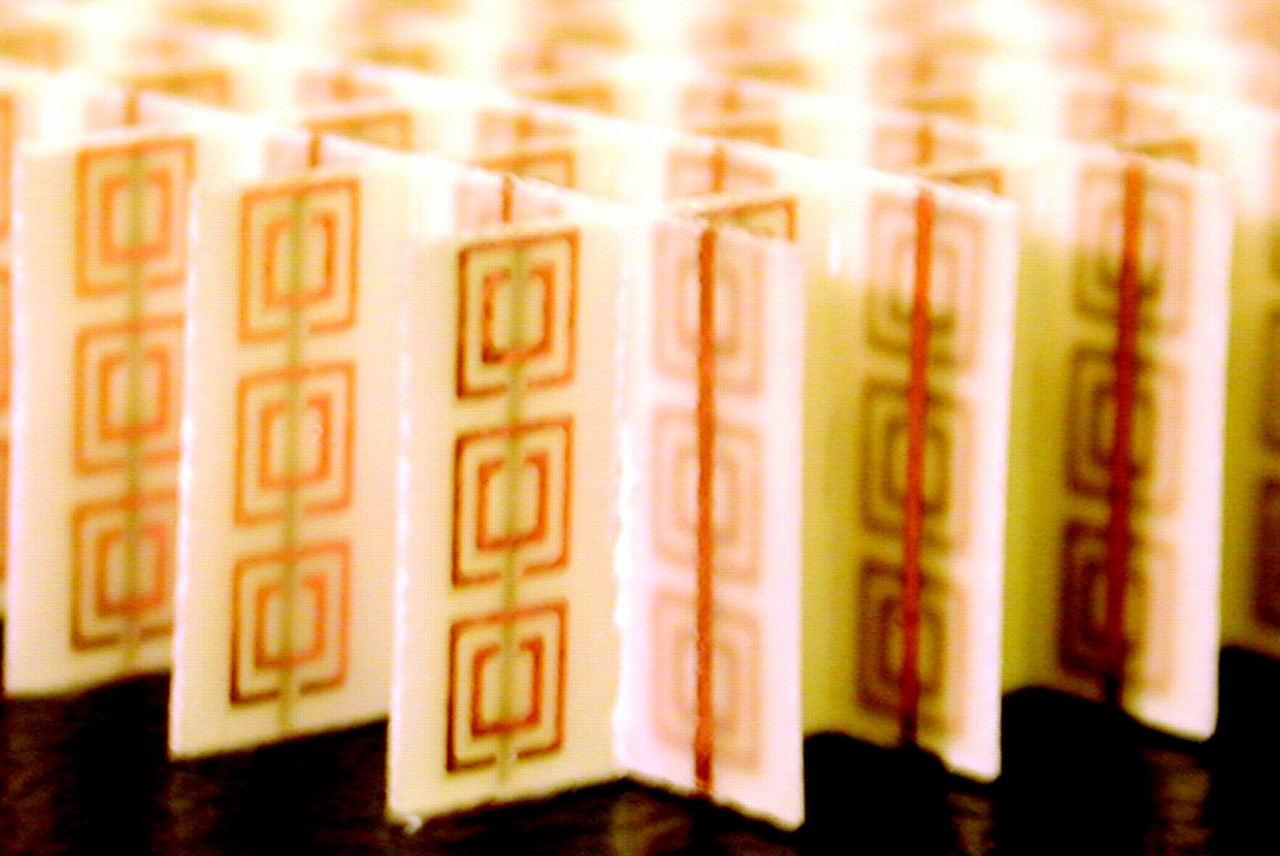
\includegraphics[width=0.8\linewidth]{sl_uvod/mm_smit.jpg}
    \caption{Експериментална реализација метаматеријала са негативними индексом~\cite{smith:00}.}
    \label{uvod:mm_smit}
\end{figure}
Прошло је више од тридесет година од Веселагове теоријске спекулације до реализације негативног индекса помоћу метаматеријала. Историјски, коришћење периодичних структура за синтезу диелектричне константе у микроталасној техници датира из педесетих година прошлог века, када су биле познате под термином „вештачки диелектрици`` (\foreign{artificial dielectric})~\cite{rotman1962plasma}. Пендри је предложио коришћење резонатора у облику прстена са процепом, тзв. сплит ринг резонатор, СРР (\foreign{split-ring, SRR}) за синтезу негативне пермеабилности~\cite{pendri:99}. Комбинацијом ова два приступа, фабриковани су метаматеријали који испољавају негативни индекс преламања у микроталасном опсегу~\cite{smith:00}.

Метаматеријал $<=>$ негативни индекс? Можда нешто рећи о томе докле су стигли са свим будалаштинама?

\section{Метаматеријали и водови}

\subsection{Дуални вод}

\begin{figure}[h]
    \centering
    \subfloat[]{
    \begin{tikzpicture}[scale=0.9]
        \ctikzset{tripoles/mos style/arrows}
        \draw 
            (-2,0) to [short] ++(0.75,0)
            to [L=$L$] ++(2.5,0)
            to [short] ++(0.75,0)


            (-1.25,0) to [C=$C$] ++(0,-2)
            node [ground] {}

            (1.25,0) to [C=$C$]++(0,-2)
            node [ground] {}

            ;
        \draw[dashed]
            (-2,0) -- ++(-1,0)
            (2,0) -- ++(1,0)
            ;
        \draw[<->] (-1.25,1) -- (1.25,1) node[midway,above] {$l$};
        \draw[densely dashed] (-1.25,0) -- ++(0,1.2)
            (1.25,0) -- ++(0,1.2);


    \end{tikzpicture}\label{uvod:rhvod}}\hfil
    \subfloat[]{
    \begin{tikzpicture}[scale=0.9]
        \ctikzset{tripoles/mos style/arrows}
        \draw 
            (-2,0) to [short] ++(0.75,0)
            to [C=$C$] ++(2.5,0)
            to [short] ++(0.75,0)


            (-1.25,0) to [L=$L$] ++(0,-2)
            node [ground] {}

            (1.25,0) to [L=$L$]++(0,-2)
            node [ground] {}

            ;
        \draw[dashed]
            (-2,0) -- ++(-1,0)
            (2,0) -- ++(1,0)
            ;

        \draw[dashed]
            (-2,0) -- ++(-1,0)
            (2,0) -- ++(1,0)
            ;
        \draw[<->] (-1.25,1.2) -- (1.25,1.2) node[midway,above] {$l$};
        \draw[densely dashed] (-1.25,0) -- ++(0,1.4)
            (1.25,0) -- ++(0,1.4);
    \end{tikzpicture}\label{uvod:lhvod}}
    \caption{Елементарна ћелија, дужине $l$, обичног вода (а) и дуалног (б).}
    %\label{fig:}
\end{figure}
Паралелно са развојем тродимензионалних метаматеријала, појавио се алтернативни концепт за реализацију негативног индекса преламања, односно инверзних таласа, на бази теорије водова~\cite{bib2,bib4,bib3}. Наиме, постоји аналогија између Максвелових једначина и једначина телеграфичара за водове, где напон одговара електричном пољу, а струја магнетном. Елементарна секција вода испуњеног „нормалним`` диелектриком (са $n>0$) приказана је на сл.~\ref{uvod:rhvod}. Размотримо дуалну структуру, на којој су замењена места реактивних елемената (сл.~\ref{uvod:lhvod}). Применом теорије периодичних структура~\cite{pozar2009microwave}, можемо одредити фазну константу простирања, $\beta$, и Блохову импедансу, $Z_B$:
\begin{align}
    \cos{\beta l} & = 1 - \frac{\omega_c^2}{2\omega^2},\\%деф. дужину ћелије!!
    Z_b & = \sqrt{\frac{L}{C}\left(1-\frac{\omega_c^2}{\omega^2}\right)},
\end{align}
где је $\omega_c = \nicefrac{2}{\sqrt{LC}}$. Ако је ћелија много мања од таласне дужине, важи $\omega\ll\omega_c$. У том случају се горњи изрази могу апроксимирати као:
\begin{align}
    \beta l & = -\frac{\omega_c}{\omega},\\
    Z_B & = \sqrt{\frac{L}{C}} \equiv Z_C,
\end{align}
где је $Z_C$ карактеристична импеданса вода испуњеног обичним диелектриком. У овој апроксимацији се може показати да су параметри ефективног диелектрика, који би испуњавао овакав вод, негативни~\cite{markes_knjiga}.

Дисперзиони дијаграми...

\subsection{Композитни водови}

\begin{figure}[h]
    \centering
    \begin{tikzpicture}[scale=0.9]
        \ctikzset{tripoles/mos style/arrows}
        \draw 
            (-2,0) 
            to [L=$L_R$] ++(2.0,0)
            to [C=$C_L$] ++(2.0,0)


            (-2.0,0) -- ++(0,-1)
            -- ++(-1,0)
            to [C=$C_R$] ++(0,-2)
            -- ++(1,0)
            node [ground] {}

            (-2,-1)-- ++(1,0)
            to [L=$L_L$] ++(0,-2)
            -- ++(-1,0)


            (2.0,0) -- ++(0,-1)
            -- ++(-1,0)
            to [C=$C_R$] ++(0,-2)
            -- ++(1,0)
            node [ground] {}

            (2,-1)-- ++(1,0)
            to [L=$L_L$] ++(0,-2)
            -- ++(-1,0)

            (-2,0) -- ++(-1,0)
            (2,0) -- ++(1,0)

            ;

        \draw[dashed]
            (-3,0) -- ++(-1,0)
            (3,0) -- ++(1,0)
            ;

    \end{tikzpicture}
    \caption{Композитни вод.}
    \label{uvod:crlh}
\end{figure}
\begin{figure}[h]
    \centering
    \subfloat[]{\begin{tikzpicture}
        \draw[] (-3,3) -- (-3,-3) node[below] {$-\pi$}
            -- (0,-3) node[below] {$\beta l$}
            -- (3,-3) node[below] {$\pi$} -- ++(0,6);
        \draw[->] (0,-3) -- (0,3.2) node[right] {$\omega$};
        %\draw[scale=0.5,domain=-3:3,smooth,variable=\x,blue] plot ({\x},{\x*\x});
        %\draw[scale=0.5,domain=-3:3,smooth,variable=\y,red]  plot ({cos(\y)},{\y});
        %\draw[scale=0.5,domain=-3:3,smooth,variable=\y,red]  plot (\y,{cos(\y)});
        \draw [domain=-3:0, samples=50, blue] plot (\x,{-1.8+0.5*cos(pi*\x r/3)}) node[right] {$\omega_s$};
        \draw [domain=-3:0, xshift=3cm, samples=50, red] plot (\x,{1.2+1.1*cos(pi*\x r/3)});
        \draw[red] (0,0.0) node[left] {$\omega_p$};
    \end{tikzpicture}\label{uvod:d_nebalans} }\hfill
    \subfloat[]{\begin{tikzpicture}
        \draw[] (-3,3) -- (-3,-3) node[below] {$-\pi$}
            -- (0,-3) node[below] {$\beta l$}
            -- (3,-3) node[below] {$\pi$} -- ++(0,6);
        \draw[->] (0,-3) -- (0,3.2) node[right] {$\omega$};
        %\draw[scale=0.5,domain=-3:3,smooth,variable=\x,blue] plot ({\x},{\x*\x});
        %\draw[scale=0.5,domain=-3:3,smooth,variable=\y,red]  plot ({cos(\y)},{\y});
        %\draw[scale=0.5,domain=-3:3,smooth,variable=\y,red]  plot (\y,{cos(\y)});
        %\draw [domain=-3:0, samples=50, blue] plot (\x,{-1.8+0.5*cos(pi*\x r/3)}) node[right] {$\omega_s$};
        \draw [domain=-3:3, samples=50, olive] plot (\x,{1.6*sin(pi*\x r/6)});
        \draw[olive] (0,0.0) node[below right] {$\omega_0$};
    \end{tikzpicture}\label{uvod:d_balans} }
    \caption{Дисперзија фазне константе простирања на композитном воду.}
    %\label{fig:}
\end{figure}
Директна реализација дуалног вода са сл.~\ref{uvod:lhvod} у пракси била би могућа само на веома ниским учестаностима, када је могуће занемарити ефекте простирања. У микроталасном опсегу, неопходно је постојање обичног вода као носиоца простирања таласа, који се затим оптерећује реактивним елементима -- редним капацитивностима и паралелним индуктивностима. Допринос овог основног вода није могуће занемарити, одговарајућа еквивалентна шема јединичне ћелије представља комбинацију сл.~\ref{uvod:rhvod} и \ref{uvod:lhvod}, и приказана је на сл.~\ref{uvod:crlh}. У литератури су овакве структуре познате под називом \emph{композитни водови} (\foreign{composite right-/left-handed transmission line, CRLH TL}). Параметри дуалне структуре су $C_L$ и $L_L$, док $C_R$ и $L_R$ одговарају воду носиоцу. Применом теорије периодичних структура, добијају се следећи изрази за дисперзиону релацију:
\begin{align}
    \cos{\beta l} & = 1 - \frac{\omega^2}{2\omega_R^2}\left( 1 - \frac{\omega_s^2}{\omega^2} \right)\left( 1 - \frac{\omega_p^2}{\omega^2} \right),\label{uvod:beta_crlh} \\
    Z_B & = \sqrt{\frac{L_R}{C_R}\frac{1-\frac{\omega_s^2}{\omega^2}}{1-\frac{\omega_p^2}{\omega^2}} - \frac{L_R^2\omega^2}{4}\left( 1 - \frac{\omega_s^2}{\omega^2} \right)^2},
\end{align}
где су
\begin{align}
    \omega_R & = \frac{1}{\sqrt{L_R C_R} },\\
    \omega_L & = \frac{1}{\sqrt{L_L C_L} },
\end{align}
резонансе обичног и дуалног вода, респективно, и
\begin{align}
    \omega_s & = \frac{1}{\sqrt{L_R C_L} },\\
    \omega_p & = \frac{1}{\sqrt{L_L C_R} },
\end{align}
представљају резонантне фреквенције у редној и паралелној грани композитног вода.

%%%%%%%%%%%%%%%%%%%%%%%%%%%%%%%%%%%%%%%%%%%%%
%  коментар где је лефт, а где рајт хендид  %
%%%%%%%%%%%%%%%%%%%%%%%%%%%%%%%%%%%%%%%%%%%%%
Тражењем реалних решења (\ref{uvod:beta_crlh}) испоставља се да постоје две фреквентне зоне простирања, раздвојене процепом, као што је приказано на сл.~\ref{uvod:d_nebalans}. Границе процепа су одређене учестаностима $\omega_s$ и $\omega_p$, између којих не постоје реална решења за $\beta$. Уколико размотримо специјалан случај $\omega_s = \omega_p$, процеп неће постојати, и дисперзија добија изглед као на сл.~\ref{uvod:d_balans}. Овај случај у литератури је познат као \emph{балансни композитни вод}, и занимљив је за многе примене, зато што омогућава манипулацију са фазним померајем на воду, задржавајући стабилну карактеристичну импедансу.

\begin{figure}[h]
    \centering
    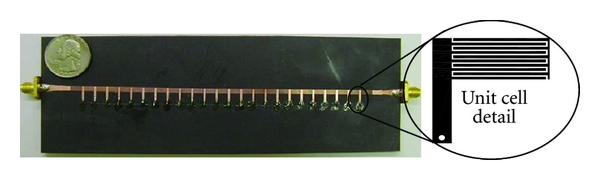
\includegraphics[width=1.0\linewidth]{sl_uvod/crlh_kalo.jpg}
    \caption{Пример композитног вода~\cite{caloz2005}.}
    \label{uvod:crlh_kalo} 
\end{figure}
Приликом реализације композитних структура, најпре је потребно одабрати основни вод – носилац. Иако је у принципу могуће користити било коју врсту вода, због лакоће фабрикације и интеграције најчешће се бирају планарни водови, као што су микрострип или копланарни таласовод. Затим се врши избор реактивних компоненти за реализацију дуалне структуре, за шта се могу користити готове компоненте са концентрисаним параметрима или дистрибуиране компоненте у техници водова. У првом случају су димензије реактивних елемената мање, па је самим могуће остварити већи опсег у коме се структура понаша као ефективно хомогена. С друге стране, вредности доступних реактанси су ограничене на оне које нуди произвођач, и интеграција са водом (најчешће лемљењем) компликује фабрикацију и уноси потенцијалне грешке. Дистрибуиране компоненте се лакше фабрикују, раде на вишим учестаностима, али потребно је водити рачуна о њиховој величини како би се добила ефективно хомогена структура.

Пример реализације композитног вода, са капацитивностима реализованим преко интердигиталних кондензатора, а индуктивностима помоћу уземљених огранака вода, дат је на сл.~\ref{uvod:crlh_kalo}. Овакве структуре су коришћене за бројне практичне апликације, које представљају унапређење у односу на раније познато стање, између осталих минијатуризоване делитеље/сабираче снаге~\cite{caloz2004novel}; подешавање импедансе у опсегу који је недоступан помоћу класичних водова~\cite{damm2007electrically}; антене са ,,цурећим`` таласом (leaky-wave), које се могу скенирати „уназад“~\cite{roig2013liquid}. Такође, концепт дуалног вода може се проширити у две димензије, за синтезу планарних метаматеријала~\cite{grbic2004overcoming,798001}.

\subsection{Резонантни приступ}%

Поступак синтезе дуалних водова, описан у претходној секцији, у литератури је познат под називом \emph{нерезонантни}, зато што се за постизање негативних вредности параметара користе реактивни елементи, који немају резонансе у опсегу од интереса. Могућ је и други приступ, \emph{резонантни}, где се водови и таласоводи периодично спрежу са подталасним резонаторима, као што су сплит ринг и сродне топологије. У том случају, еквивалентна шема ћелије биће нешто сложенија него на сл.~\ref{uvod:crlh}, али са веома сличним карактеристикама – такође испољава композитну природу, и поседује опсеге са негативним и нормалним параметрима~\cite{markes_knjiga}.

\bibliographystyle{babplai3}
\bibliography{ref}

\end{document}


%\documentclass[12pt,oneside]{book}

%% Маргине, проред и тако то
%\usepackage[a4paper, margin=30mm]{geometry}
%\renewcommand{\baselinestretch}{1.5}

%% Фонтови, енкодинг
%\usepackage[]{mathtext}
%\usepackage[T2A, TS1]{fontenc}
%\usepackage[utf8]{inputenc}
%\usepackage[serbianc]{babel}
%% \usepackage[fixlanguage]{babelbib}
%% \selectbiblanguage{serbian}

%\usepackage{graphicx}

%\usepackage[tight,footnotesize]{subfloat}

\newcommand{\sirina}{\columnwidth}
\newcommand{\sirinab}{\columnwidth}
\newcommand{\sirinac}{0.48\columnwidth}
\newcommand{\SkalaA}{0.3}
\newcommand{\SkalaB}{0.3}
\newcommand{\SkalaC}{0.3}
\newcommand{\subscript}[1]{\ensuremath{_{\textrm{#1}}}}

%\usepackage{amsmath}

%\usepackage{url}

%\usepackage{siunitx}
%\sisetup{output-decimal-marker = {,}}

%\begin{document}
\newcommand{\ga}{\Gamma\Pi}

\chapter{Екстракција параметара}

\section{Увод}

Као што је већ речено у уводном поглављу, основна претпоставка која се везује за метаматеријале јесте да се понашају као хомогена средина на опсегу учестаности од интереса. У складу с тиме могу се описати помоћу ефективних параметара, као што су пермитивност, $\varepsilon$ и пермеабилност, $\mu$. Јасно је да је одређивање вредности ових параметара од прворазредног значаја за карактеризацију метаматеријала, као и за њихову примену. Постоји више начина како се ово може урадити; у једноставнијим случајевима, могуће је аналитичко решење~\cite{pendri:99}, или постоји могућност нумеричког усредњавања п\^{о}ља. Ипак, најчешће се користи поступак \emph{екстракције} ових параметара, базиран на инверзији параметара расејања, добијених мерењем или симулацијом.

Постоји више варијанти самог поступка, али у принципу све оне представљају варијације тзв. процедуре Николсона-Роса-Вира (НРВ), која је развијена за карактеризацију природних материјала~\cite{Nicol:70,Weir:74}, а затим прилагођена за метаматеријале~\cite{Smith:02,Markos:03}. Укратко се може описати на следећи начин. Узорак (мета)материјала, који се испитује, се замени изотропним хомогеним медијумом одговарајућих димензија. Затим се одреде параметри расејања хомогеног медијума, у функцији од његових параметара $\varepsilon$ и $\mu$. На крају се тражи решење које се поклапа са измереним или симулираним параметрима расејања. У случају водова на бази метаматеријала, могуће је применити у суштини исти приступ, само је потребно извршити нормализацију на карактеристичну импедансу вода~\cite{Mao:05}.

Један од проблема са стандардном НРВ процедуром екстракције настаје уколико узорак метаматеријала испољава асиметричну рефлексију. Очигледно, изотропни медијум као модел не може да репродукује такво својство, пошто је он увек симетричан. Још један проблем са изотропним медијумом (донекле повезан са претходним) јесте што он имплицира међусобну независност електричне и магнетне поларизације (тј. да $\vec{D}$ зависи само од $\vec{E}$-поља, а $\vec{B}$ од $\vec{H}$), али из литературе је познато да неки често коришћени резонатори у метаматеријалима, као што је сплит-ринг, имају истовремени електрични и магнетни одзив, другим речима одговарајући диполи су спрегнути~\cite{marques}. Није увек могуће занемарити ову спрегу, што зависи од оријентације сплит-ринг резонатора и начина њихове побуде.

Оба поменута ефекта, асиметрична рефлексија и спрега магнетне и електричне индукције могу се моделовати помоћу бианизотропног медијума, што је већ предложено у литератури за случај 2Д и 3Д метаматеријала~\cite{chen:05,kriegler,shalaev}. У радовима \cite{bian_mtt,bian_physcr} је показано како се бианизотропни еквивалентни медијум може применити на водове на бази метаматеријала. У наставку ће бити дат преглед најважнијих резултата. У секцији~\ref{sekc2} разматрају се особине водова испуњених бианизотропним медијумом, изведени су електрични параметри секције таквог вода, на основу којих се, у инверзном поступку екстракције, могу добити ефективни параметри медијума. У секцији \ref{sekc4} је процедура екстракције примењена на јединичне ћелије које се састоје од микрострип вода спрегнутог са сплит-ринг резонаторима са асиметрично постављеним процепима. У секцији \ref{sekc4} предсављена је провера валидности поступка, на основу симулације вода са хомогеним диелектриком, који поседује добијене ефективне параметре.

%дискусија око нефизичких резонанси, нег. вредности парам.

\section{Генералисана процедура екстракције}\label{sekc2}
\subsection{Вод испуњен бианизотропним диелектриком}
Размотримо вод (тј. структуру која подржава вођени ТЕМ талас), чија оса је постављена дуж $z$ координате. Претпоставимо да се вод налази у хомогеном бианизотропном медијуму, описаном следећим конститутивним релацијама ($\varepsilon_0$, $\mu_0$ и $c$ су пермитивност, пермеабилност и брзина светлости у вакууму):
\begin{equation}\label{const}
\begin{split}
\vec{D} & = \varepsilon_0\varepsilon \vec{E} + \bar{\xi}\vec{H}\\
\vec{B} & = \bar{\zeta} \vec{E} + \mu_0\mu \vec{H};
\end{split}
\end{equation}
где је
\begin{equation}\label{bian}
\bar{\xi} = \bar{\zeta} = \frac{1}{c}
\begin{bmatrix}
0 & -ju & 0 \\
ju & 0 & 0 \\
0 & 0 & 0
\end{bmatrix}.
\end{equation}
Услов реципрочности је задовољен јер важи $\bar{\xi}=-\bar{\zeta}^T$~\cite{shivola}. Примећујемо да се тензори разликују у односу на претходно објављене~\cite{marques, chen:05, kriegler, shalaev} који поседују само један вандијагонални елемент. Разлог за ову разлику лежи у чињеници да вод има нехомогену структуру поља у трансверзалној равни, за разлику од раванског таласа. Форма~(\ref{bian}) осигурава да магнетно-електрична спрега не зависи од поларизације трансверзалног поља, што доводи до много једноставнијег решења него у случају да то није испуњено, што ће постати јасно касније.

%Сада, претпоставимо да вођени талас пропагира дуж $z$ осе, при чему све величине зависе од $z$ координате као $e^{-\gamma z}$; а од времена као\footnote{Комплексне величине су дефинисане као, нпр. $n=n'-jn''$.} $e^{j\omega t}$. Такође претпостављамо да је талас ТЕМ типа, тј. да су аксијалне компоненте $\vec{E}$ и $\vec{H}$ вектора једнаке нули. Сада можемо извести следеће релације из роторских Максвелових једначина:
\begin{equation}\label{vrot}
\begin{split}
\vec{i_z}\times \left( -\gamma\vec{H} \right) = j\omega\vec{D},\\
\vec{i_z}\times \left( -\gamma\vec{E} \right) = -j\omega\vec{B};
\end{split}
\end{equation}
где је $\vec{i_z}$ орт у правцу $z$-осе. Конститутивне релације могу бити преписане као:
\begin{equation}\label{vkonst}
\begin{split}
\vec{D} = \varepsilon_0\varepsilon \vec{E} + \vec{i_z}\times \left( j\frac{u}{c}\vec{H} \right),\\
\vec{B} = \mu_0\mu \vec{H} + \vec{i_z}\times \left( j\frac{u}{c}\vec{E} \right).
\end{split}
\end{equation}
Комбиновањем (\ref{vrot}) и (\ref{vkonst}) добија се:
\begin{align}
(\gamma - \frac{\omega}{c} u)\left( \vec{i_z}\times\vec{H} \right) &= -j\omega\varepsilon_0\varepsilon\vec{E};\label{roth}\\
(\gamma + \frac{\omega}{c} u)\left( \vec{i_z}\times\vec{E} \right) &= j\omega\mu_0\mu\vec{H}.\label{rote}
\end{align}
Комбиновање (\ref{roth}) и (\ref{rote}) даје таласну једначину:
\begin{equation}
\left(\gamma^2+\frac{\omega^2}{c^2}\left(\varepsilon\mu -u^2\right)\right)\vec{E}=0,
\end{equation}
која даје следећу дисперзиону релацију:
\begin{equation}\label{dispg}
\gamma=\pm j\frac{\omega}{c}\sqrt{\varepsilon\mu - u^2},
\end{equation}
или, пошто је $\gamma=j\frac{\omega}{c}n$,
\begin{equation}\label{dispn}
n = \pm \sqrt{\varepsilon\mu - u^2}.
\end{equation}

Различити знаци у (\ref{dispg}) и (\ref{dispn}) означавају два могућа правца простирања дуж  $z$-осе. Тачно решење за одређени смер треба изабрати у складу са критеријумом пасивности.

Карактеристична импеданса медијума (тј. однос између јачина електричног и магнетног поља) може се добити заменом (\ref{dispg}) у (\ref{roth}), што даје (нормализовано на $z_0=\sqrt{\mu_0 / \varepsilon_0}$):
\begin{equation}\label{dispz}
z_{1,2} = \frac{n\pm ju}{\varepsilon},
\end{equation}
где $z_{1,2}$ одговара пропагацији дуж позитивног и негативног смера $z$-осе, респективно. Из (\ref{dispz}) је јасно да импеданса има различите вредности за пропагацију у различитим смеровима, што даје различиту рефлексију (?).

Из (\ref{roth}) и (\ref{rote}) закључујемо да су вектори електричног и магнетног поља пропорционални и међусобно нормални у свакој тачки трансверзалне равни. Такође, вектори поларизације $\vec{D}$ и $\vec{B}$ су пропорционални $\vec{E}$ и $\vec{H}$, респективно. Дакле, Максвелове једначине које одређују расподелу поља у трансверзалној равни се неће променити, осим фактора пропорционалности, у односу на вод у ваздуху. Последично, карактеристична импеданса вода (тј. однос струје и напона) ће се променити пропорционално:
\begin{equation}
Z_{c1,2} = z_{1,2}Z_{вазд.},
\end{equation}
где је $Z_{вазд.}$ карактеристична импеданса вода у ваздуху. Алтернативно, карактеристичне импедансе могу да се запишу као
\begin{equation}\label{zceta}
Z_{c1,2} = Z_c \pm \eta,\quad Z_c = \frac{Z_{c1}+Z_{c2}}{2}
\end{equation}
где $Z_c = \frac{n}{\varepsilon} Z_{вазд.}$ представља средњу вредност, а $\eta = \frac{ju}{\varepsilon} Z_{вазд.}$, на основу једначине (\ref{dispz}), представља одступање од средње вредности.% Овај облик ће бити коришћен касније, зато што омогућава једноставнију формулацију.

\subsection{Услови за негативни индекс преламања}

У свом познатом раду, Веселаго је показао да ће материјал без губитака имати негативни индекс преламања у случају када су $\varepsilon$ и $\mu$ истовремено негативни~\cite{veselago_cir}. Међутим, овај услов није егзактан када се узму у обзир губици, присутни у свим природним материјалима. Показано је да је неопходни услов у случају са губицима~\cite{mccall,mccall2}:
\begin{equation}\label{usl_std}
\varepsilon'\mu''+\mu'\varepsilon'' < 0.
\end{equation}

Овај услов изведен је користећи стандардну дисперзиону релацију, $n=\sqrt{\varepsilon\mu}$. За бианизотропне медијуме, међутим, правилна дисперзиона релација дата је са~(\ref{dispn}), и услов за негативни индекс преламања мора бити изведен полазећи од ње.

Да би се добио негативни индекс преламања, потребно је имати решење~(\ref{dispn}) са $n''>0$ и $n'<0$ (да би се осигурао позитивни ток снаге и негативна фазна брзина, респективно)~\cite{mccall}. Другим речима, $n$ се мора налазити у другом квадранту комплексне равни. Ово имплицира да се $n^2$ нужно налази у доњој полуравни, тј. $\mathrm{Im}\{n^2\}<0$. Заменом~(\ref{dispn}) добијамо
\begin{equation}\label{usln}
\varepsilon'\mu''+\mu'\varepsilon'' < 2u'u''.
\end{equation}
Важна последица~(\ref{usln}) је да показује да је могуће имати истовремено и $\varepsilon'$ и $\mu'$ негативно, а ипак не добити негативни индекс рефракције уколико је $u'u''$ негативно.

\subsection{Мрежни параметри секције вода}
Претпоставимо да имамо секцију вода дужине $l$, испуњене бианизотропним медијумом параметара $\varepsilon$, $\mu$ и $u$. Можемо посматрати ову секцију као двопортну мрежу, која се може описати параметрима расејања ($S$-параметрима), или било којом другом врстом мрежних параметара (импедансни, адмитансни, итд.). Користићемо опис помоћу $ABCD$ параметара, који се показао најпогоднијим за ову дискусију. Матрица $ABCD$ параметара дефинисана је на следећи начин~\cite{Pozar:05}:
\begin{equation}\label{abcd_osn}
\begin{bmatrix} V_1 \\ I_1 \end{bmatrix} = 
\begin{bmatrix} A & B \\ C & D \end{bmatrix}
\begin{bmatrix} V_2 \\ I_2 \end{bmatrix},
\end{equation}
са референтним смеровима за струје и напоне означеним на сл.~\ref{fpole}.
\begin{figure}[!t]
\centering
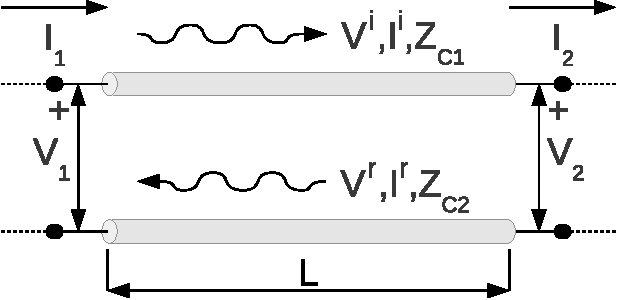
\includegraphics[width=0.5\columnwidth]{slike/sekcija.pdf}
\caption{Секција асиметричног вода дужине $L$}
\label{fpole}
\end{figure}

Циљ нам је да добијемо $ABCD$ параметре у функцији од параметара вода изведених у претходној секцији, наиме константе пропагације $\gamma$ (исте за оба правца простираања), дефинисане у (\ref{dispg}), и карактеристичних импеданси $Z_{c1}$ и $Z_{c2}$ (за инцидентни и рефлектовани талас, респективно), дефинисане у (\ref{zceta}). У сврху тога, представићемо стање на воду у било којој тачки помоћу напона инцидентног и рефлектованог таласа, $V^i$ и $V^r$, респективно. Релација између ових напона на портовима 1 и 2, у матричном облику, биће:
\begin{equation}\label{modal_basis}
\begin{bmatrix} V^i_1 \\ V^r_1 \end{bmatrix} =
\begin{bmatrix} e^{\gamma l} & 0 \\ 0 & e^{-\gamma l} \end{bmatrix}
\begin{bmatrix} V^i_2 \\ V^r_2 \end{bmatrix}.
\end{equation}
Укупни напон и струја у било којој тачки вода могу се представити као:
\begin{equation}\label{slicnost}
\begin{bmatrix} V \\ I \end{bmatrix} =
\begin{bmatrix} 1 & 1 \\ \frac{1}{Z_{c1}} & -\frac{1}{Z_{c2}} \end{bmatrix}
\begin{bmatrix} V^i \\ V^r \end{bmatrix} = 
Q\begin{bmatrix} V^i \\ V^r \end{bmatrix}.
\end{equation}
Инверзна релација је:
\begin{equation}\label{slicnost2}
\begin{bmatrix} V^i \\ V^r \end{bmatrix} =
Q^{-1}\begin{bmatrix} V \\ I \end{bmatrix}.
\end{equation}
%By substituing (\ref{slicnost2}) into (\ref{modal_basis}), we obtain:
%\begin{equation}
%Q^{-1}\begin{bmatrix} V_1 \\ I_1 \end{bmatrix} =
%\begin{bmatrix} e^{\gamma l} & 0 \\ 0 & e^{-\gamma l} \end{bmatrix}
%Q^{-1}\begin{`bmatrix} V_2 \\ I_2 \end{bmatrix}.
%\end{equation}
Заменом (\ref{slicnost2}) у (\ref{modal_basis}) и множењем са $Q$ са леве стране добијамо $ABCD$ матрицу:
\begin{equation}\label{decomp}
ABCD = Q\begin{bmatrix} e^{\gamma l} & 0 \\ 0 & e^{-\gamma l} \end{bmatrix}Q^{-1},
\end{equation}
која се, после замене вредности $Q$ и мало сређивања, своди на:
\begin{equation}\label{abcd}
\begin{bmatrix}
\cosh{\gamma l} + \dfrac{\eta}{Z_c}\sinh{\gamma l } & \left( Z_c - \dfrac{\eta^2}{Z_c} \right) \sinh{\gamma l} \\
\dfrac{\sinh{\gamma l}}{Z_c} & \cosh{\gamma l} - \dfrac{\eta}{Z_c}\sinh{\gamma l }
\end{bmatrix}.
\end{equation}
Може се видети из (\ref{abcd}) да када је $\eta = 0$, односно у симетричном случају, $ABCD$ се своде на случај вода са обичним диелектриком.

\subsection{Екстракција параметара}
Параметри расејања ($S$-параметри) се најчешће добијају као резултат мерења или ЕМ симулације, и могу се једнозначно трансформисати у $ABCD$ матрицу~\cite{Pozar:05}. Када је добијемо, лако се види из (\ref{abcd}) да се ефективни параметри могу добити на следећи начин:
\begin{align}
\gamma & = \pm \cosh^{-1}\frac{A+D}{2},\label{a2gama}\\
Z_c & = \frac{\sinh{\gamma l}}{C} = \pm\frac{1}{C}\sqrt{1 - \left( \frac{A+D}{2}\right)^2},\label{a2zc}\\
\eta & = \frac{A-D}{2C}.\label{a2eta}
\end{align}
%Уколико је јединична ћелија симетрична\footnote{Симетрија имплицира $A=D$ за $ABCD$ параметре, и $S_{11}=S_{22}$ за $S$-параметре.}, можемо заменити $S$-параметре и поједноставити изразе тако да се добије
%\begin{eqnarray}
%\gamma = \pm\frac{1}{L}\cosh^{-1}\frac{1-S_{11}^2+S_{21}^2}{2S_{21}},\label{s2gama} \\
%Z_c = \pm \sqrt{\frac{(1+S_{11})^2-S_{21}^2}{(1-S_{11})^2-S_{21}^2}}\label{s2zc},
%\end{eqnarray}
%и $\eta = 0$, што се слаже са претходним резултатима за НРВ процедуру, што је било очекивано~\cite{Smith:02, Mao:05, Chen:04}. %ovaj pasus treba dide dole

Неколико додатних коментара је потребно у вези датих релација. Најпре, знак у (\ref{a2gama}) треба изабрати у складу са критеријумом пасивности, 
\begin{equation}\label{pasivnost}
\mathrm{Re}\left\lbrace\gamma\right\rbrace > 0.
\end{equation}
Ипак, остаје проблем гранања функције $\cosh^{-1}{z}$, који доводи до неодређености у имагинарном делу $\gamma$ (односно, у реалном делу $n$). Ово је последица чињенице да је немогуће разликовати промену фазе од $\phi$ до $\phi + 2k\pi, k\in Z$. Један приступ за решавање овог проблема је коришћење Крамерс-Кронигових релација да се процени тачна грана~\cite{Szabo:10}.

У већини претходних извештаја~\cite{Nicol:70, Weir:74, Smith:02, Markos:03, Mao:05}, знак карактеристичне импедансе у (\ref{a2zc}) или (\ref{s2zc}) се бира на основу критеријума $\mathrm{Re}\{Z_c\}>0$ или сличног, који може бити веома осетљив на мале нумеричке грешке~\cite{Chen:04}. Ипак, јасно се види из (\ref{a2zc}) да је знак каркатеристичне импедансе повезан са знаком константе простирања у (\ref{a2gama}), дакле, само један критеријум је довољан, као што је показано у~\cite{Chen:04}.

\subsection{Ефективни параметри еквивалентног медијума}
Када је одређена константа простирања, $\gamma$, и карактеристична импеданса еквивалентног вода, $Z_{c1,2}$, индекс преламања, $n$, и карактеристична импеданса еквивалентног медијума, $z_{1,2}$, се лако добијају
\begin{equation}\label{nz}
n = -j\frac{c}{\omega}\gamma,\quad z_{1,2}=\frac{Z_{c1,2}}{Z_{вазд.}}.
\end{equation}
Ефективни параметри бианизотропног медијума, $\varepsilon$, $\mu$ и $u$ могу се изразити преко $n$ и $z_{1,2}$ преуређењем (\ref{dispn}) и (\ref{dispz}):
\begin{equation}\label{effp}
\begin{split}
	\varepsilon = \frac{2n}{z_1+z_2},\quad
	\mu = 2n\frac{z_1z_2}{z_1+z_2},\quad
	u = -jn\frac{z_1-z_2}{z_1+z_2}.
\end{split}
\end{equation}
Комбинација (\ref{nz}) и (\ref{effp}) са изразима који их повезују са $S$-параметрима изведеним раније омогућава ектстракцију ефективних параметара из симулираних или експерименталних података. Ове релације ћемо надаље обележавати као генералисани поступак ($ГП$).

Још једна могућност за опис асиметричних јединичних ћелија је коришћење $\varepsilon$ и $\mu$ који зависе од смера простирања таласа. Они се могу добити као
\begin{equation}
\varepsilon_{1,2}=\frac{n}{z_{1,2}};\quad \mu_{1,2}=nz_{1,2}.
\end{equation}
Иако је математички еквиваленан претходном, овај приступ нема директну физичку интерпретацију. Међутим, показаће се као изузетно користан за валидацију ефективних параметара у секцији~\ref{sekc4}, због чега ће бити укључен у примере екстракције, где ће се реферисати као генералисани поступак за инцидентни талас на порту 1 и порту 2 ($ГП_1$ и $ГП_2$, респективно).

\subsection{Николсон-Рос-Вир процедура са усредњавањем}

Како би се заобишло ограничење НРВ процедуре у случају асиметричних узорака, предложено је коришћење геометријске средине рефлексије, $S_{11ср}=\sqrt{S_{11}S_{22}}$~\cite{smith:05}; овај поступак ће бити означаван као $НРВ_{ср}$. Како би се јасније представиле сличности и разлике између $НРВ_{ср}$ и овде излаганог метода, изрази (\ref{a2gama})--(\ref{a2zc}) ће бити приказани преко $Ѕ$-параметара:
\begin{equation}\label{phy_gama}
\gamma=\mp\frac{1}{L}\cosh^{-1}{\frac{1-S_{11}S_{22}+S_{12}^2}{2S_{12}}},%=\mp\frac{jc}{\omega l}\cosh{\frac{1-S_{11avg}^2+S_{12}^2}{2S_{12}}},
\end{equation}
\begin{equation}\label{phy_zc}
Z_{c} = \frac{2S_{12}\sqrt{1-\left( \frac{1-S_{11}S_{22}+S_{12}^2}{2S_{12}} \right)^2}}{1-S_{11}-S_{22}+S_{11}S_{22}-S_{12}^2}. (избачено Z_0?)
\end{equation}
Уколико је ћелија симетрична, $Ѕ_{11}=Ѕ_{22}$, горњи изрази ће се поједноставити у
\begin{eqnarray}
\gamma = \pm\frac{1}{L}\cosh^{-1}\frac{1-S_{11}^2+S_{21}^2}{2S_{21}},\label{s2gama} \\
Z_c = \pm \sqrt{\frac{(1+S_{11})^2-S_{21}^2}{(1-S_{11})^2-S_{21}^2}}\label{s2zc}.
\end{eqnarray}
Суштински, $НРВ_{ср}$ процедура се базира на замени $Ѕ_{11}$ у изразима (\ref{s2gama})--(\ref{s2zc}) са $\sqrt{Ѕ_{11}Ѕ_{22}}$. Лако се види да ће израз за константу простирања (\ref{s2gama}) приликом ове замене претворити у тачан израз (\ref{phy_gama}). С друге стране, израз за импедансу (\ref{s2zc}) неће бити еквивалентан изразу (\ref{phy_zc}), услед постојања линеарних чланова у имениоцу. Због тога ће се карактеристичне импедансе добијене помоћу два метода разликовати; при томе у случају $НРВ_{ср}$ израз није добијен полазећи од почетних дефиниција, као код ГП метода, већ донекле арбитрарним поступком усредњавања. Такође, пошто импеданса фигурише у изразима ефективних $\varepsilon$ и $\mu$, разлике ће се пренети и на њих. У наставку ће бити дато поређење екстрахованих ефективних параметара на оба начина за различите практичне случајеве, где ће бити показана већа утемељеност ГП метода у случајевима са израженом асиметријом.

\section{Асиметричне јединичне ћелије}\label{sekc3}

У овом делу се врши испитивање електромагнетних својстава метаматеријала на бази водова, који се састоји од микрострип вода спрегнутог са сплит-ринг резонаторима, постављеним са једне стране вода.

Показано је да се ротирањем појединачних сплит-рингова значајно утиче на електромагнетне особине структуре, због промене интеракције услед другачије међусобне оријентације сплит-рингова, као и другачије оријентације у односу на вод~\cite{stereo,bib9}.

Коришћењем предложеног генералисаног поступка екстракције, истраживаће се нове асиметричне јединичне ћелије реализоване на двослојном супстрату. Ивице прстенова које садрже процепе постављене су једна изнад друге, а не на супротним странама као што је то уобичајено. За разлику од уобичајеног дизајна, нови СРР-ови имају резонантне учестаности међусобно много ближе (око 500\,MHz), што је погодно за савремене бежичне системе.

Испитиваће се два типа СРР-ова: са процепима паралелним и нормалним у односу на вод. Процепи могу да се померају симетрично лево и десно у односу на центар ивице на којој се налазе, као што је приказано на сл.~\ref{fig4} за СРР-ове са паралелним процепима.

Како би се испитала ефективност предложене методе у односу на $НРВ_{ср}$ поступак, тестиране су структуре које имају слабо изражену асиметрију, код којих је процеп паралелан воду, као и оне које су наглашено асиметричне, код којих је процеп нормалан на вод.

\subsection{Јединичне ћелије са паралелним процепом}

Овај тип јединичних ћелија може имати процепе на ивицама које су ближе воду или даље од њега, као што је приказано на сл.~\ref{fig4}. Јединичне ћелије састоје се од два пара СРР-ова са процепима симетрично помереним од центра. Сваки пар се састоји од два спрегнута прстена, који се налазе један изнад другог (\foreign{broadside-coupled}). Асиметрија је узрокована само чињеницом да су процепи у различитим слојевима супстрата (горњем и доњем). Микрострип вод је повезан са масом (проводном равни) преко цилиндричне вије, пречника $R_v$, постављеном у центру ћелије између референтних равни (означених испрекиданим линијама).

Јединичне ћелије су симулиране помоћу програма WIPL-D Pro 10.0, намењеног за 3Д електромагнетну анализу~\cite{wipl}, који је базиран на методи момената; $S$-параметри су деембедовани на референтним равнима. Биће упоређена екстракција бианизотропних параметара, $ГП$, асиметрична екстракција која даје два скупа параметара, $ГП_{1,2}$ као и стандардни поступак са усредњавањем $НРВ_{ср}$.
\begin{figure}[!t]
\subfloat[]{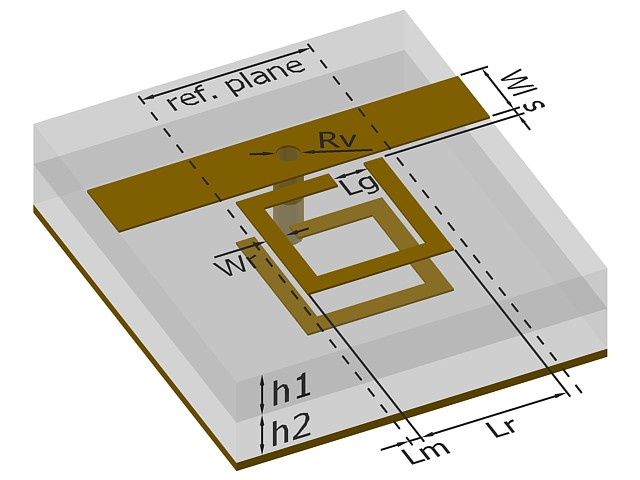
\includegraphics[width=0.45\textwidth]{slike/p1.jpeg}
\label{fig4a}}\hfill
\subfloat[]{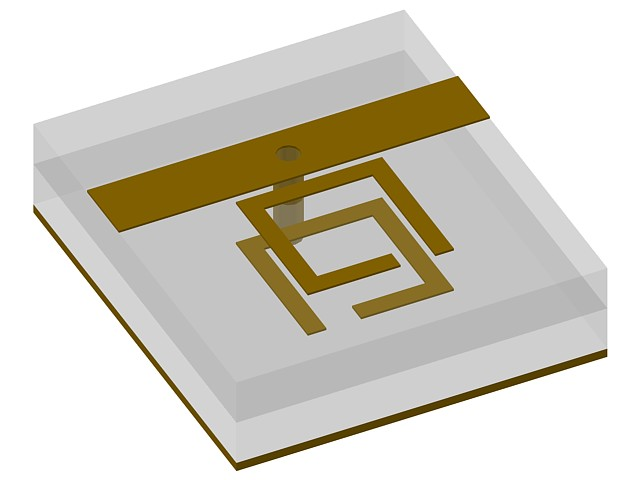
\includegraphics[width=0.45\textwidth]{slike/p2.jpeg}
\label{fig4b}}
\caption{Јединичне ћелије са процепима помереним на супротне стране у односу на средину ивице прстена: (а) процепи близу вода, (б) процепи даље од вода. Релевантне димензије: $h_1~=~0.635\,\mathrm{mm}$, $h_2=1.575\,\mathrm{mm}$, $\varepsilon_{r1}=10.2$, $\varepsilon_{r2}=2.2$, $L_r=3.15\,\mathrm{mm}$, $L_g=0.75\,\mathrm{mm}$, $L_a=2\,\mathrm{mm}$, $L_m=0.25\mathrm{mm}$, $L= L_r +2L_m$, $W_l=1.4\,\mathrm{mm}$, $W_r=0.4\,\mathrm{mm}$, $R_v=0.5\,\mathrm{mm}$, $s=0.2\,\mathrm{mm}$.}
\label{fig4}
\end{figure}

Магнитуда $S$-параметара за јединичне ћелије са процепима близу вода (сл. \ref{fig4a}) приказана је на сл.~\ref{fig5a}. Може се видети да разлика између коефицијената рефлексије $S_{11}$ и $S_{22}$ постоји само у околини прве резонансе. Екстраховани индекс преламања на сл.~\ref{fig5b} је исти код свих поступака, захваљујући погодно дефинисаној средњој вредности код $НРВ_{ср}$. Јединична ћелија испољава ,,леворуки`` опсег око \SI{5.5}{\giga\hertz}, осенчен на графику, и ,,десноруки`` опсег око \SI{6.15}{\giga\hertz}, који одговара другој резонанси.
\begin{figure}[!t]
\subfloat[]{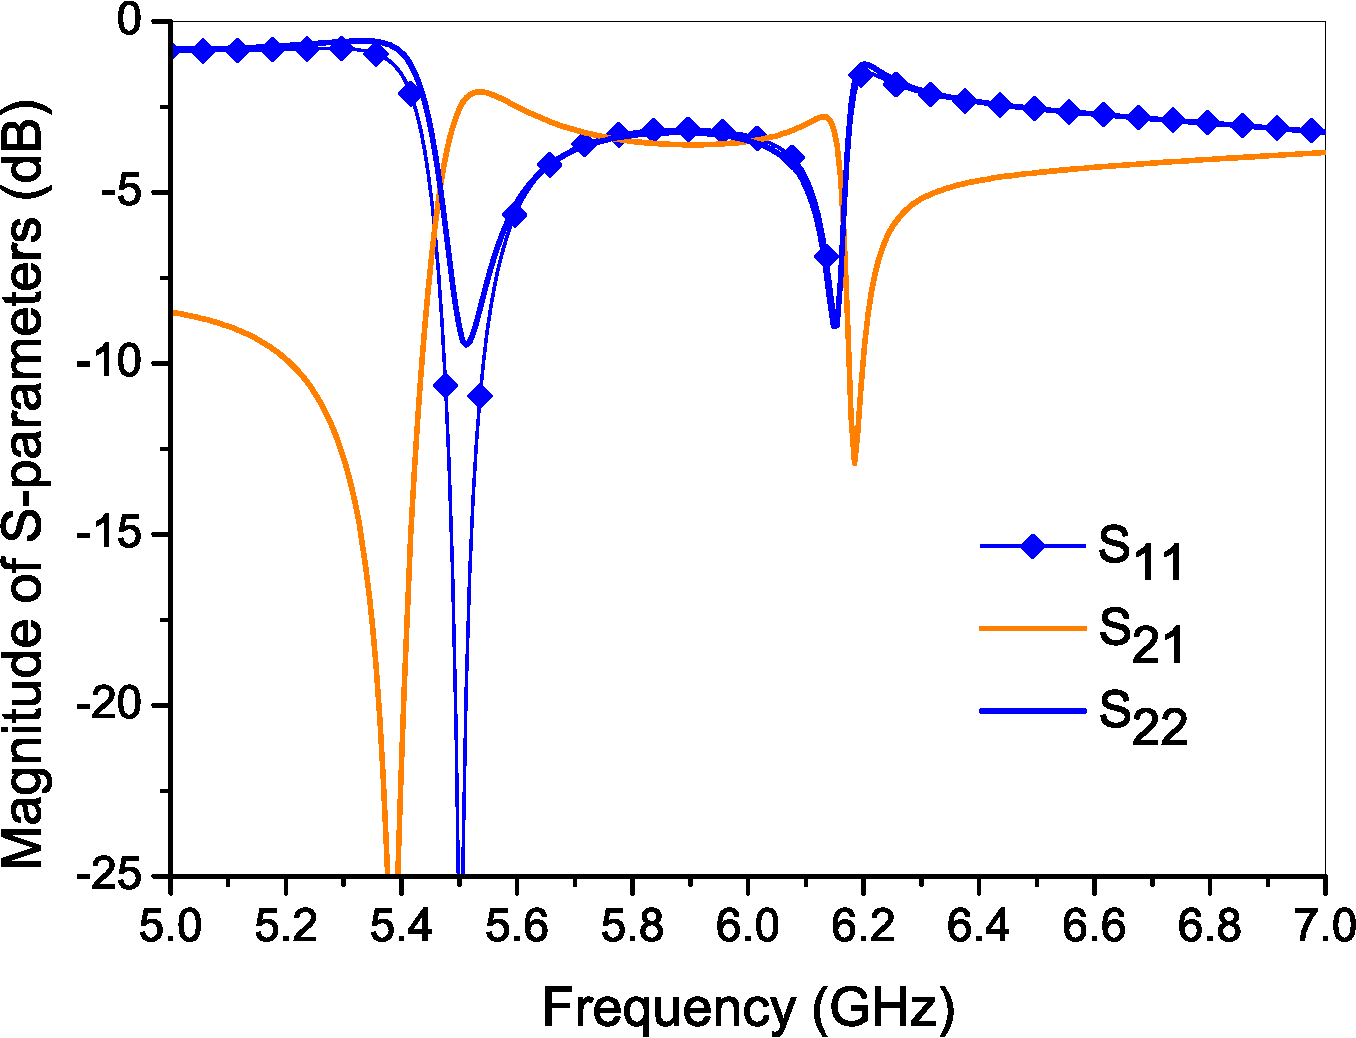
\includegraphics[scale=\SkalaA]{slike/5a.pdf}
\label{fig5a}}\hfill
\subfloat[]{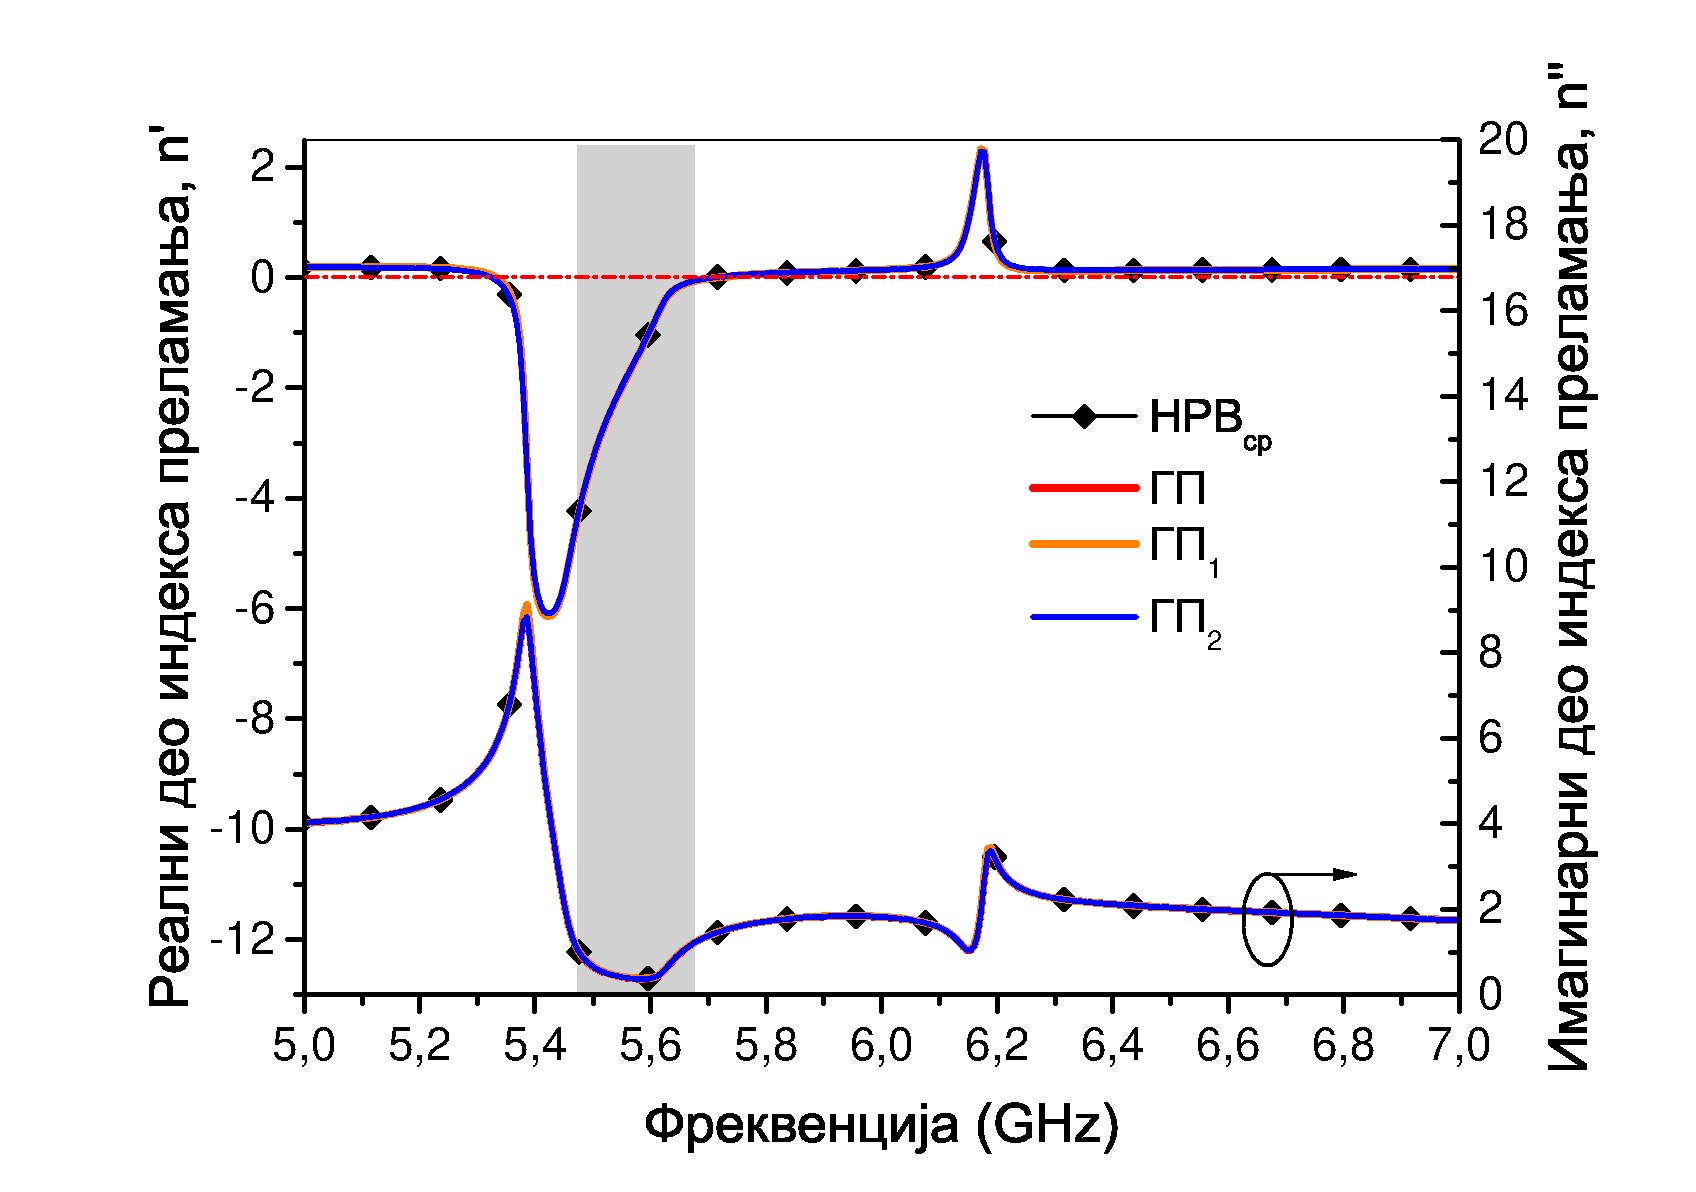
\includegraphics[scale=\SkalaA]{slike/5b.pdf}
\label{fig5b}}
\caption{Јединичне ћелије са АСРР-овима са процепом близу вода: (а) магнитуда $S$-параметара, (б) екстраховани индекс преламања. Осенчени правоугаоник означава фреквенцијски опсег са двоструко негативним параметрима.}
\label{fig5}асдф
\end{figure}адсф 

Карактеристичне импедансе, екстраховане помоћу различитих метода, су упоређене на сл.~\ref{fig7}. Може се видети да се вредности добијене помоћу $ГП$ налазе тачно између вредности добијених преко $ГП_{1,2}$, као што је очекивано на основу релације (12). Важно је истаћи да је само на првој резонанси вредност добијена $НРВ_{ср}$ методом другачија, али незнатно, од вредности добијене $ГП$ методом, што значи да асиметрија није знатно изражена.
\begin{figure}[!t]
\centering
\includegraphics[scale=\SkalaB]{slike/11a.pdf}
\caption{Карактеристична импеданса екстрахована различитим поступцима за јединичне ћелије са АСРР-овима са процепом близу вода.}
\label{fig7}
\end{figure} 

\subsection{Јединичне ћелије са процепима далеко од вода}

Јединичне ћелије са процепима даље од вода, сл.~\ref{fig4b}, имају доста другачије $Ѕ$-параметре и екстраховани индекс преламања од ћелија са процепом близу вода (видети сл.~\ref{fig8} и сл.~\ref{fig8b}). Разлика између коефицијената рефлексије на портовима 1 и 2 се јавља код друге резонансе, што је евидентно у њиховој фази на сл.~\ref{fig8c}. Екстраховани индекс преламања, приказан на сл.~\ref{fig8b}, има два ,,леворука`` опсега око \SI{5.9}{\giga\hertz} и \SI{6.35}{\giga\hertz}, који су означени осенченим правоугаоницима.
\begin{figure}[!t]
\subfloat[]{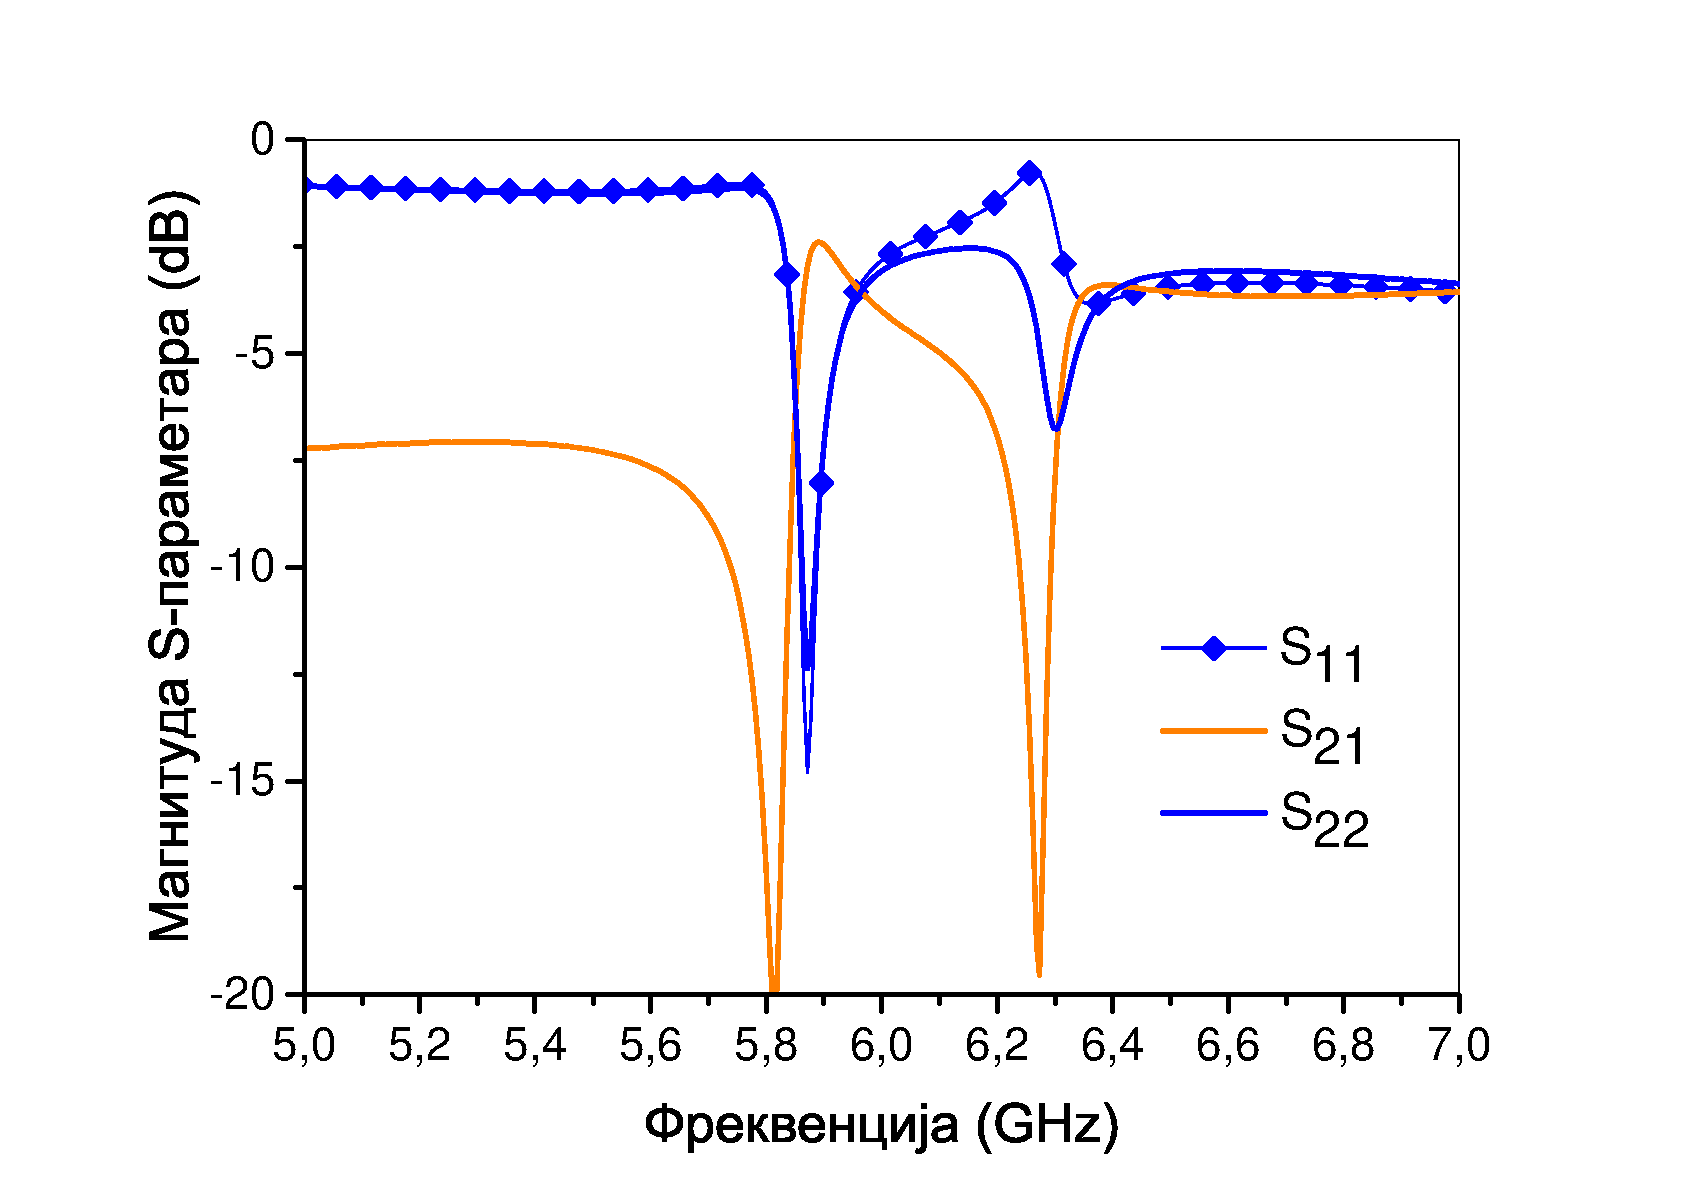
\includegraphics[scale=\SkalaA]{slike/8a.pdf}
\label{fig8a}}\hfill
\subfloat[]{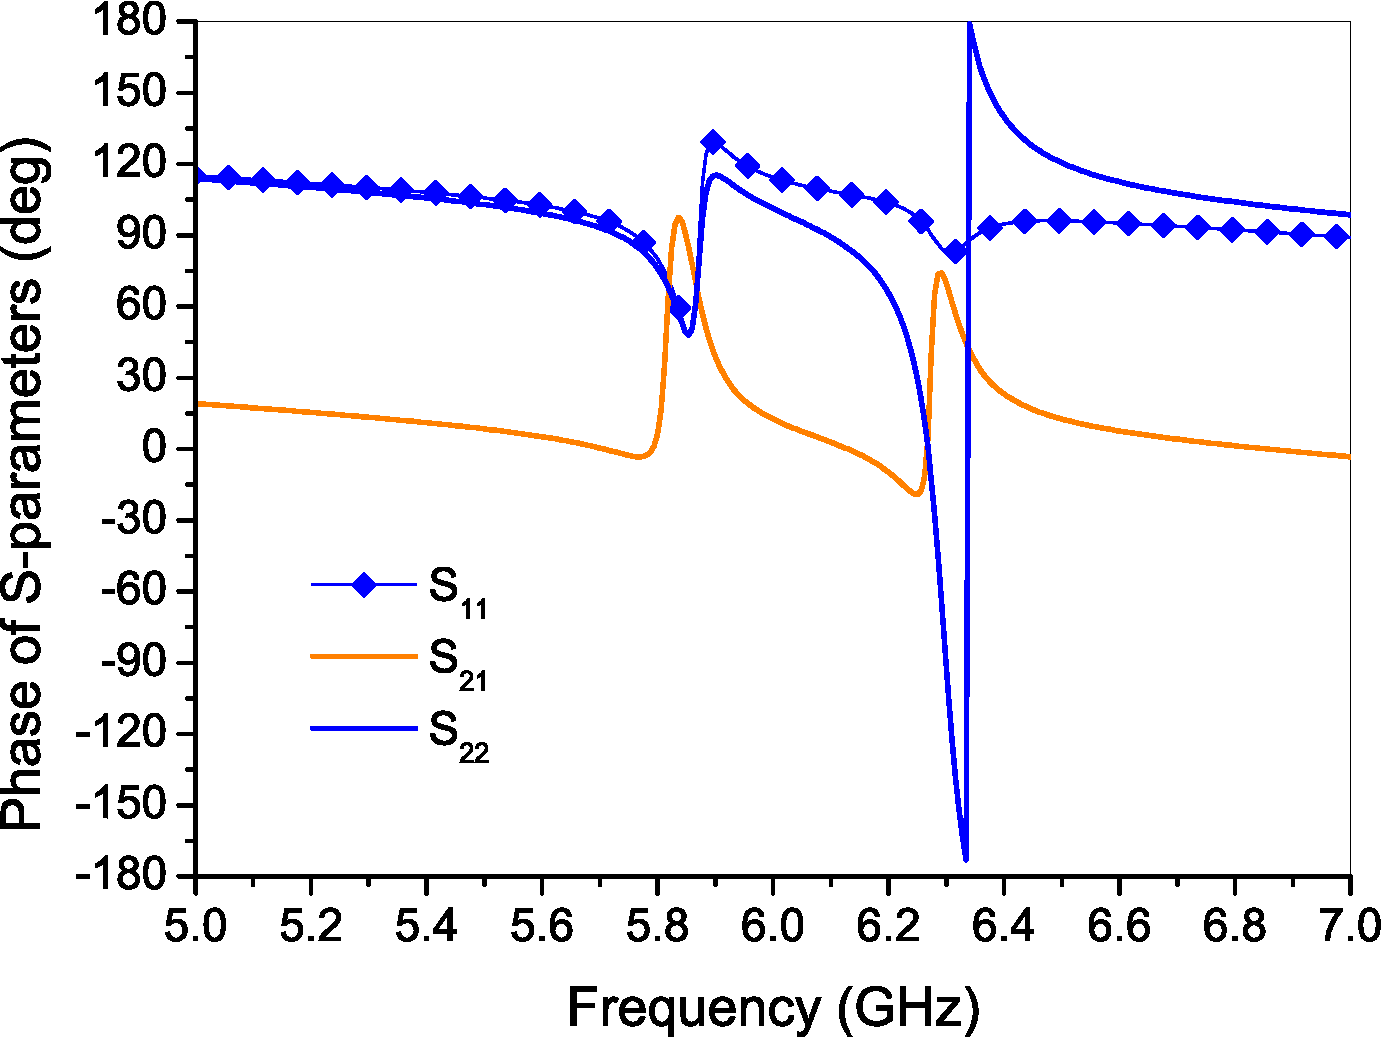
\includegraphics[scale=\SkalaA]{slike/8c.pdf}
\label{fig8c}}
\caption{Магнитуда (а) и фаза (б) $S$-параметара за АСРР-ове са процепима даље од вода.}
\label{fig8}
\end{figure}
\begin{figure}[!t]
\centering
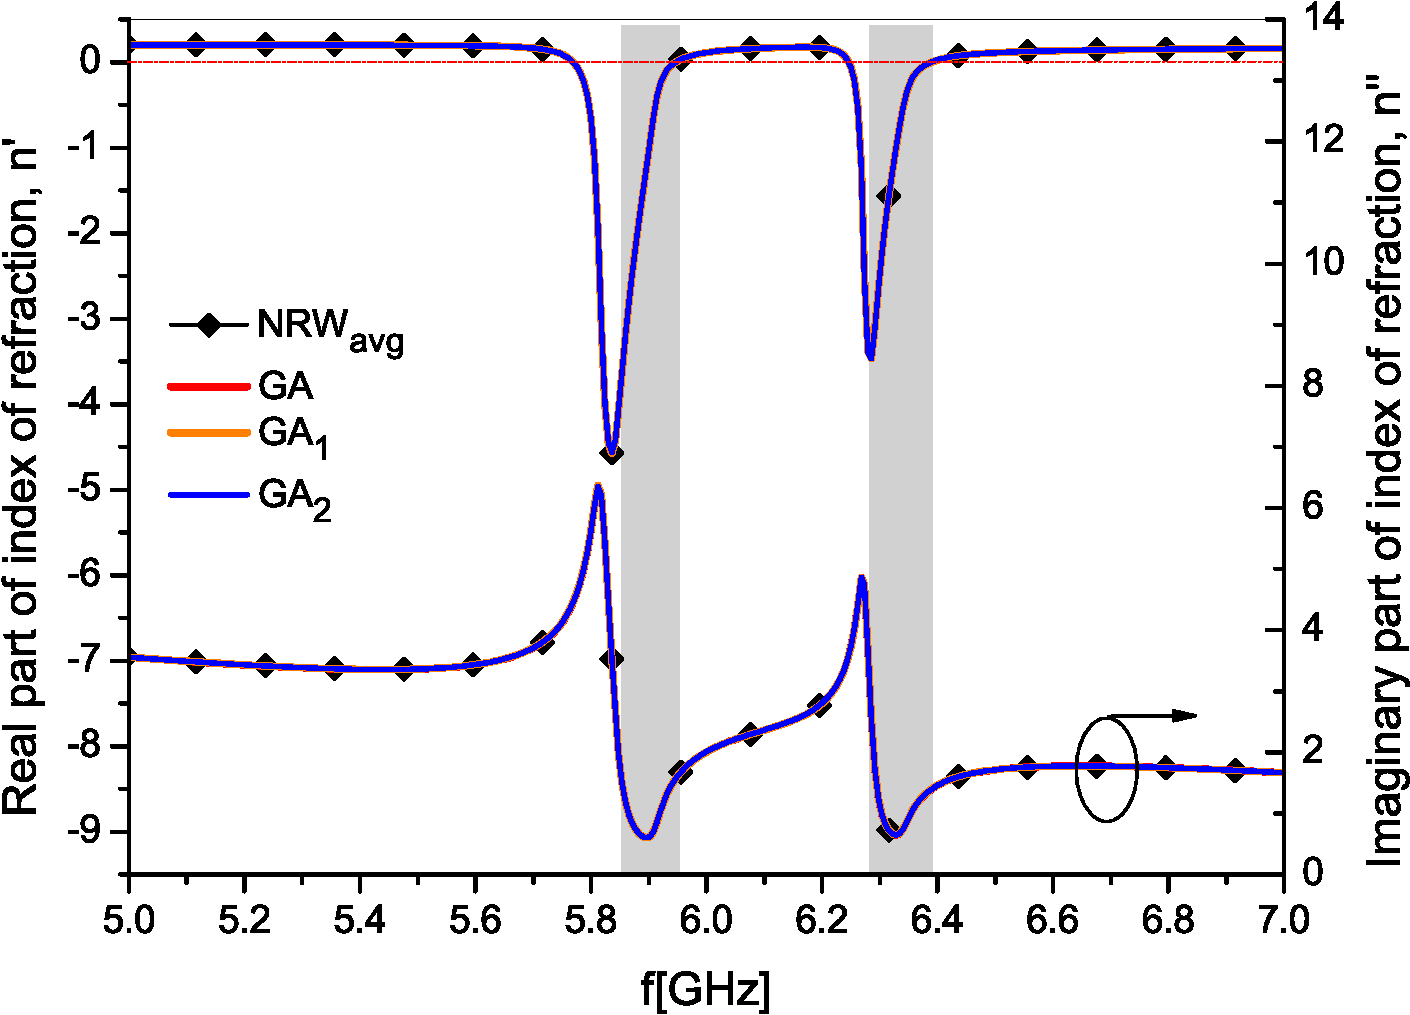
\includegraphics[scale=\SkalaB]{slike/8b.pdf}
\caption{Ефективни индекс преламања, екстрахован различитим поступцима, за јединичне ћелије са АСРР-овима са процепом даље од вода. Осенчени правоугаоници означавају фреквенцијске опсеге са двоструко негативним параметрима.}
\label{fig8b}
\end{figure} 
%\begin{figure}[!t]
%\subfloat[]{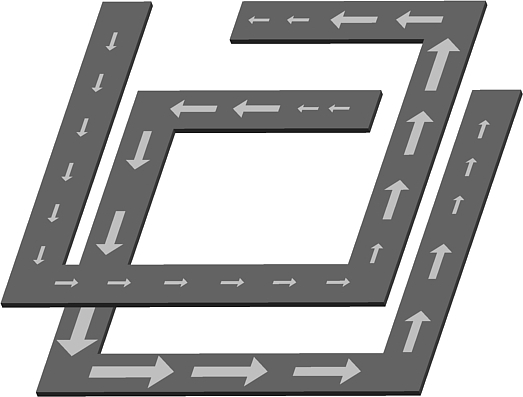
\includegraphics[width=0.45\textwidth]{slike/9a.jpeg}
%\label{fig9a}}\hfill
%\subfloat[]{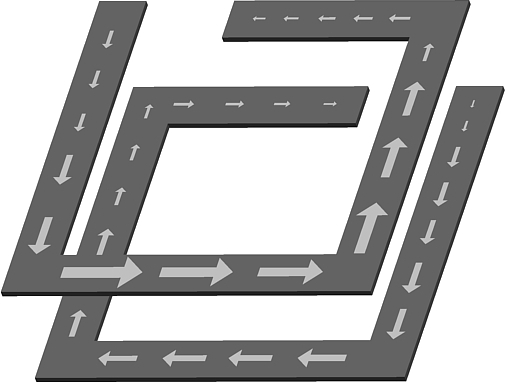
\includegraphics[width=0.45\textwidth]{slike/9b.jpeg}
%\label{fig9b}}
%\caption{Расподела струја, да ли то да убацим? Local induced current distribution at resonant frequencies: (а)~symmetric mode at $f=\SI{5.9}{\giga\hertz}$ and (б) anti-symmetric mode at $f=\SI{6.35}{\giga\hertz}$. Length of the arrows are proportional to the intensity of the current.}
%\label{fig9}
%\end{figure}

Екстрахована ефективна пермитивност, пермеабилност и карактеристична импеданса, коришћењем $ГП$, $ГП_{1,2}$ и $НРВ_{ср}$ приказани су на сл.~\ref{fig10}. Са слике се види да све методе дају исте резултате у опсегу где је одзив симетричан ($S_{11} = S_{22}$). Ефективни параметри добијени помоћу ГП и $НРВ_{ср}$ се разликују само око друге резонансе, где је асиметрија најизраженија, што је обележено осенченим правоугаоницима на сл.~\ref{fig10}. У целом опсегу учестаности од интереса ефективна пермитивност добијена $НРВ_{ср}$ и ГП методама је негативна, док ефективна пермеабилност мења знак на две резонансе које одговарају ,,леворуким`` опсезима.
\begin{figure}[!t]
\centering
\subfloat[]{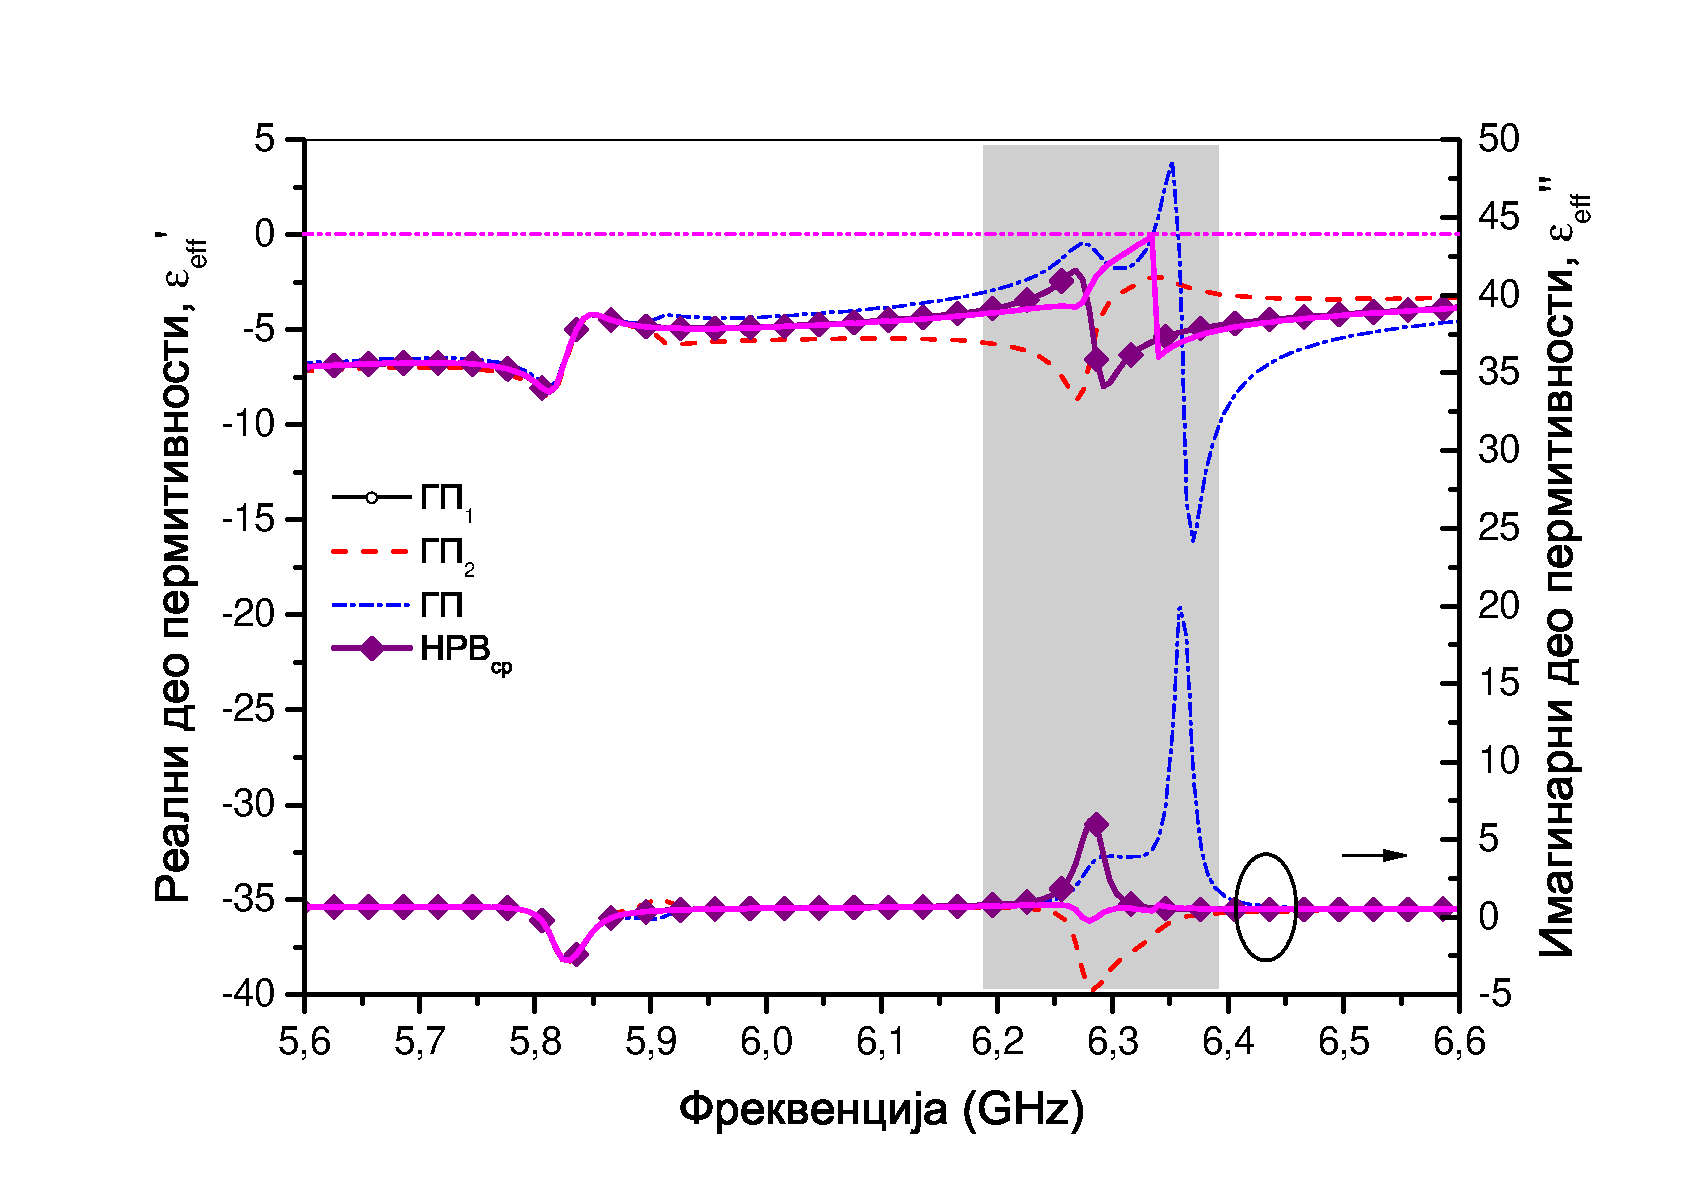
\includegraphics[width=0.6\textwidth]{slike/10a.pdf}
\label{fig10a}}\hfill
\subfloat[]{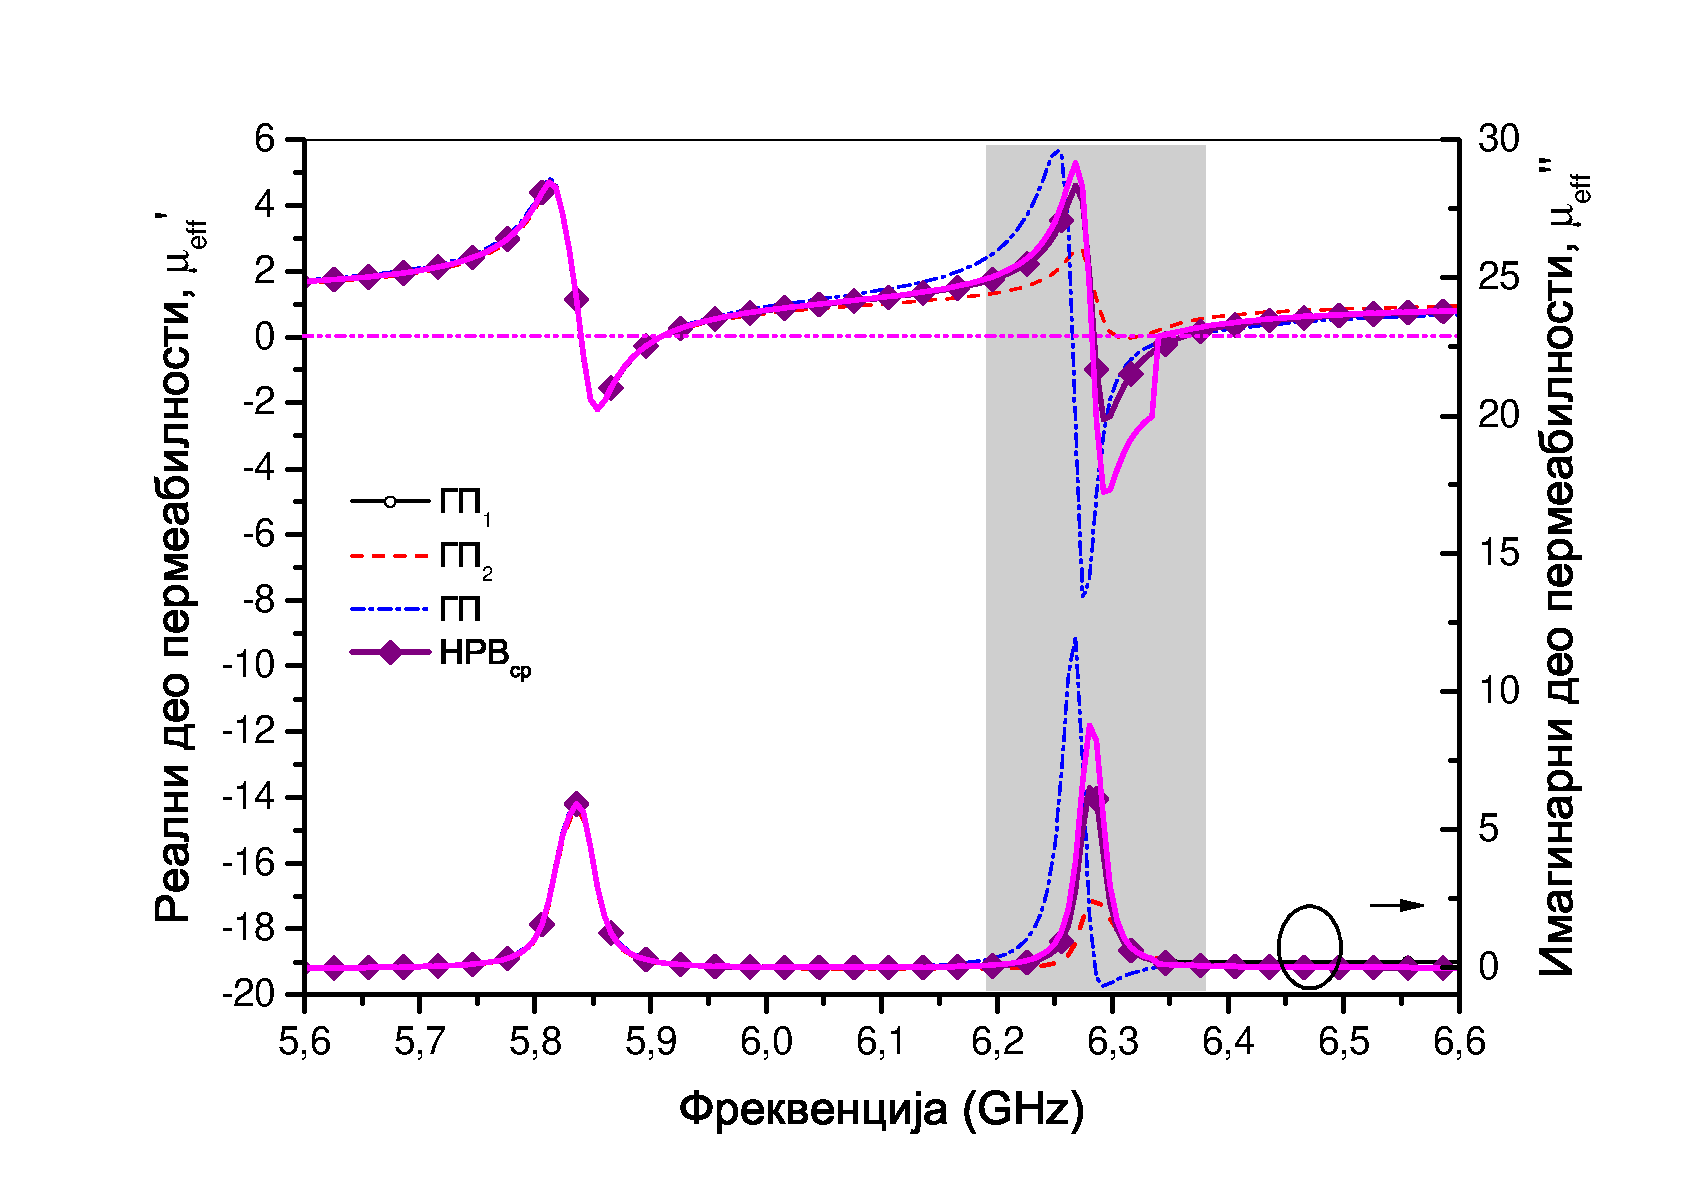
\includegraphics[width=0.6\textwidth]{slike/10b.pdf}
\label{fig10b}}\\
\subfloat[]{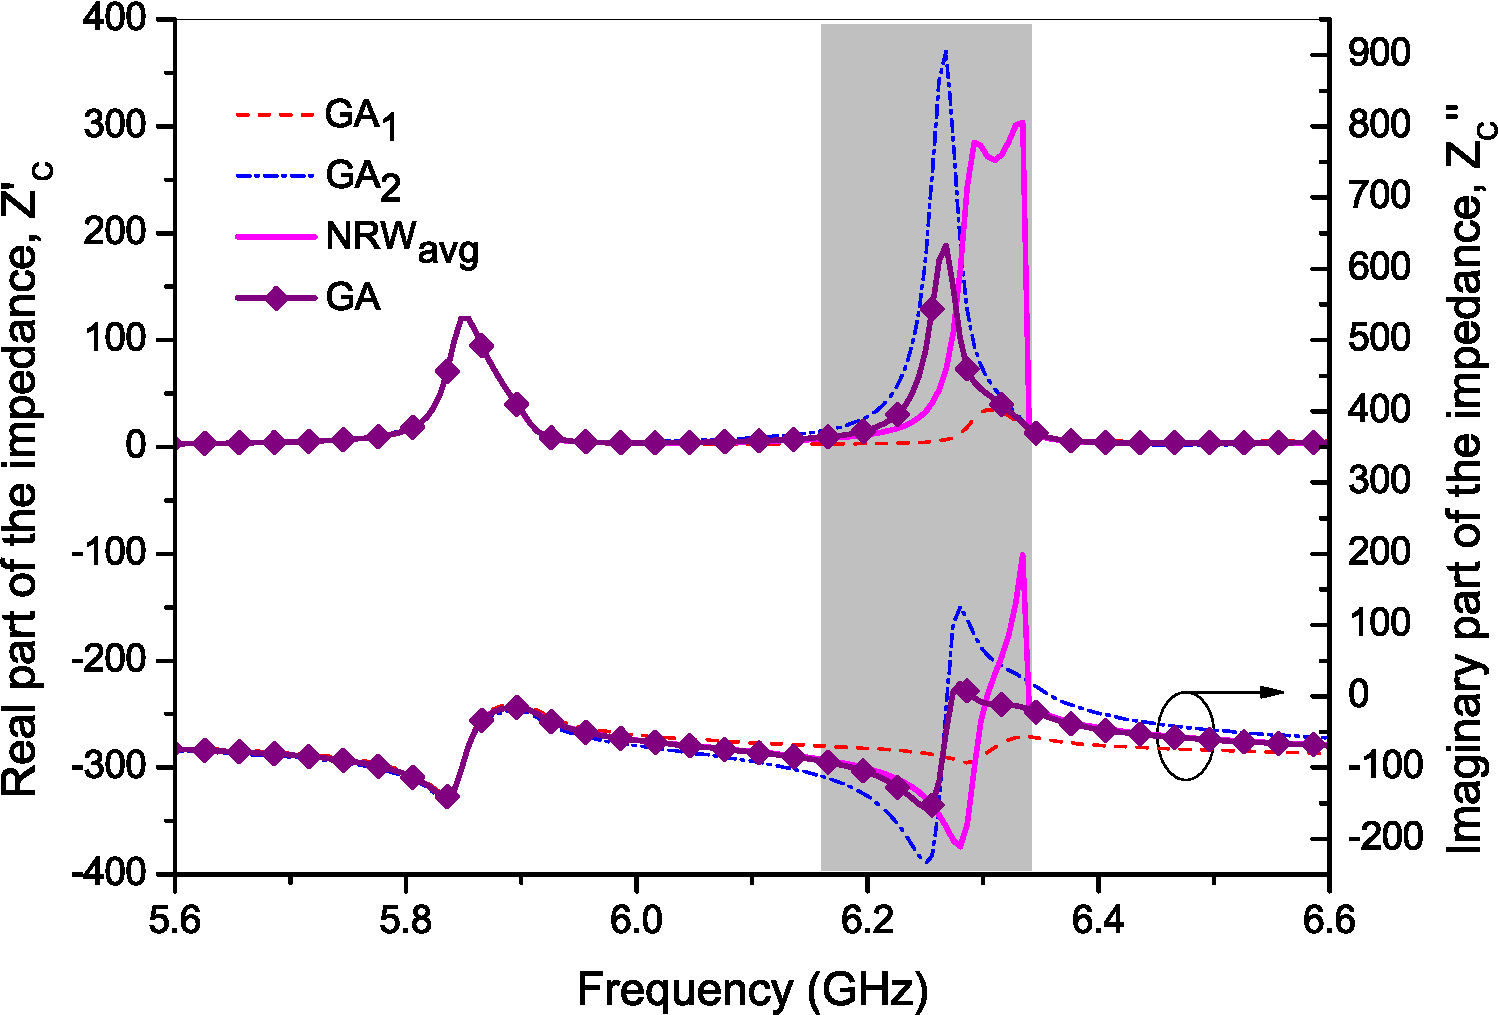
\includegraphics[width=0.6\textwidth]{slike/11b.pdf}
\label{fig11b}}
\caption{Ефективна пермитивност (а), пермеабилност (б) и карактеристична импеданса (в) екстрахована за АСРР-ове са процепима даље од вода. Осенчени правоугаоници означавају опсеге где $НРВ_{ср}$ и ГП дају различите резултате.}
\label{fig10}
\end{figure} 

%In Fig.~\ref{fig11} we compare characteristic impedances extracted using different retrieval procedures for unit cells with ASRRs. It can be seen that the different retrieval procedures give very different results at the first and second resonances for the case with gaps near and far from ML respectively. Difference is particularly pronounced if the gaps are far from ML as it is indicated by rectangular bar in Fig.~\ref{fig11b}. 
%\begin{figure}[!t]
%\subfloat[]{\includegraphics[width=\sirina]{slike/11a}
%\label{fig11a}}
%\subfloat[]{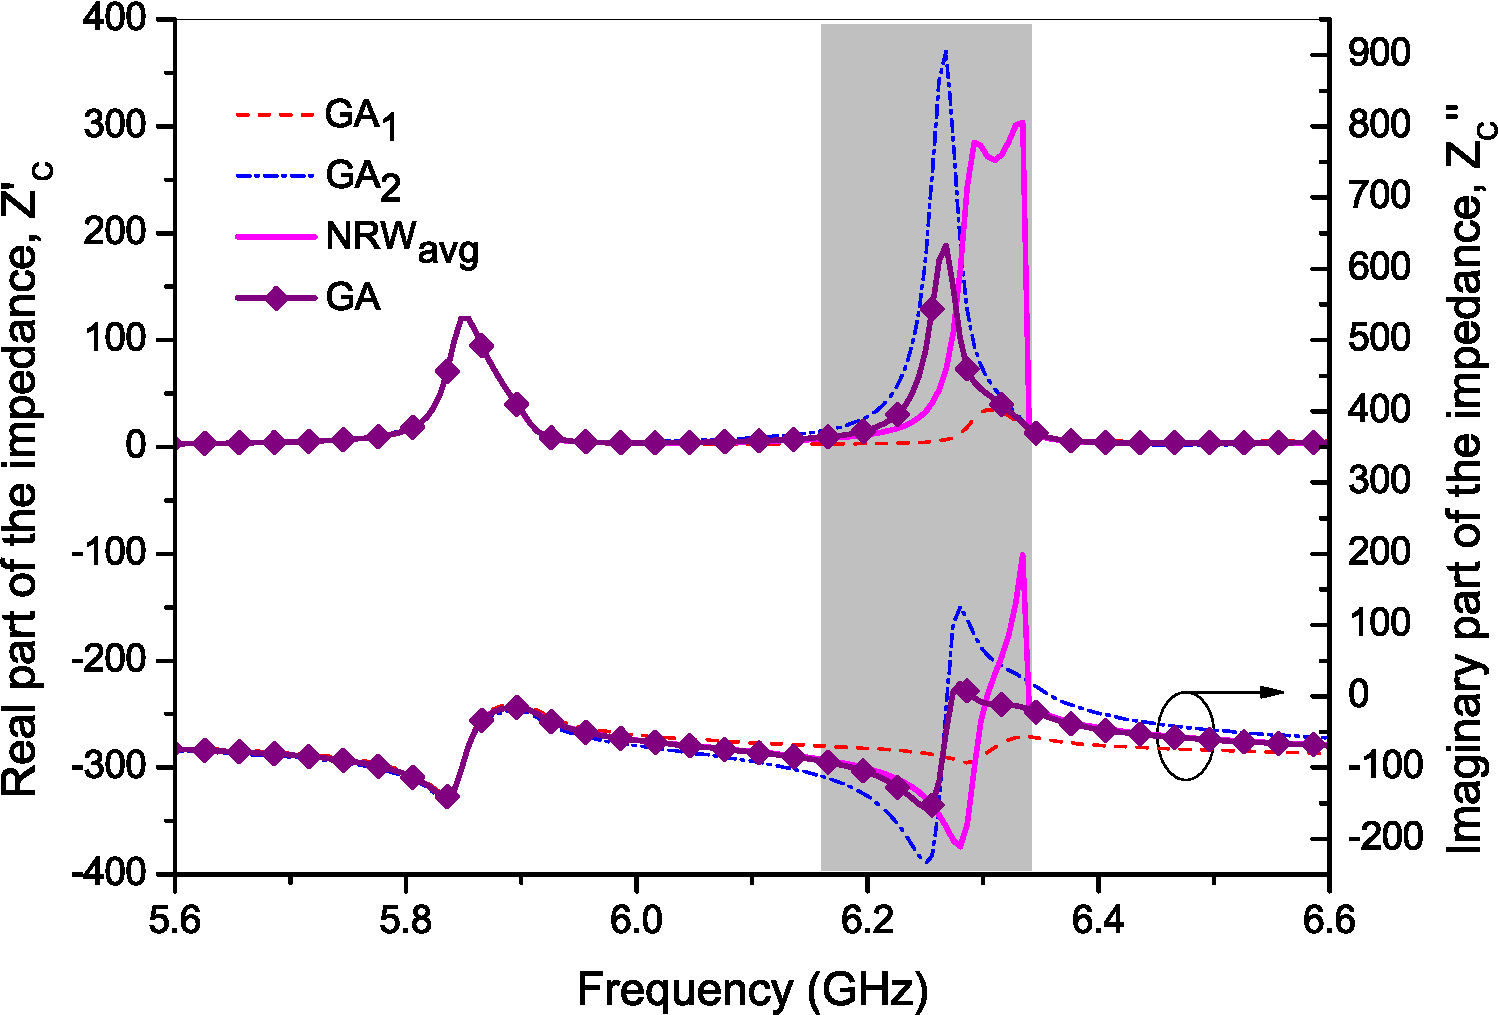
\includegraphics[width=\sirina]{slike/11b}
%\label{fig11b}}
%\caption{The effective characteristic impedance extracted using different retrieval procedures for unit cells with ASRRs: (a) with gaps near ML and (b) with gaps far from ML. Rectangular bars denote frequency range in which NRWavg and GA give different results.}
%\label{fig11}
%\end{figure} 

Генералисани поступак екстракције уводи два нова параметра, као меру асиметрије јединичне ћелије: $u$ и $\eta$. Сл.~\ref{fig12} јасно показује да јединичне ћелије са процепима даље од вода имају максималне вредности $u$ и $\eta$ параметара око три пута веће него ћелије са процепима ближе воду. Такође се види да се бианизотропија јавља у близини или прве или друге резонансе одговарајућих ћелија. Интересантно је напоменути да је бианизотропија драстично мања уколико су процепи постављени на супротним странама СРР-ова, као што је то уобичајено случај, чак и када су процепи померени од центра ивице. У том случају бианизотропија се јавља на обе резонансе.
%\begin{figure}[!t]
%\centering
%\includegraphics[scale=\SkalaB]{slike/graf_cr/11a}
%\caption{The extracted characteristic impedance extracted using different retrieval procedures for unit cell with ASRRs with gaps near ML.}
%\label{fig7}
%\end{figure} 
\begin{figure}[!t]
\centering
\subfloat[]{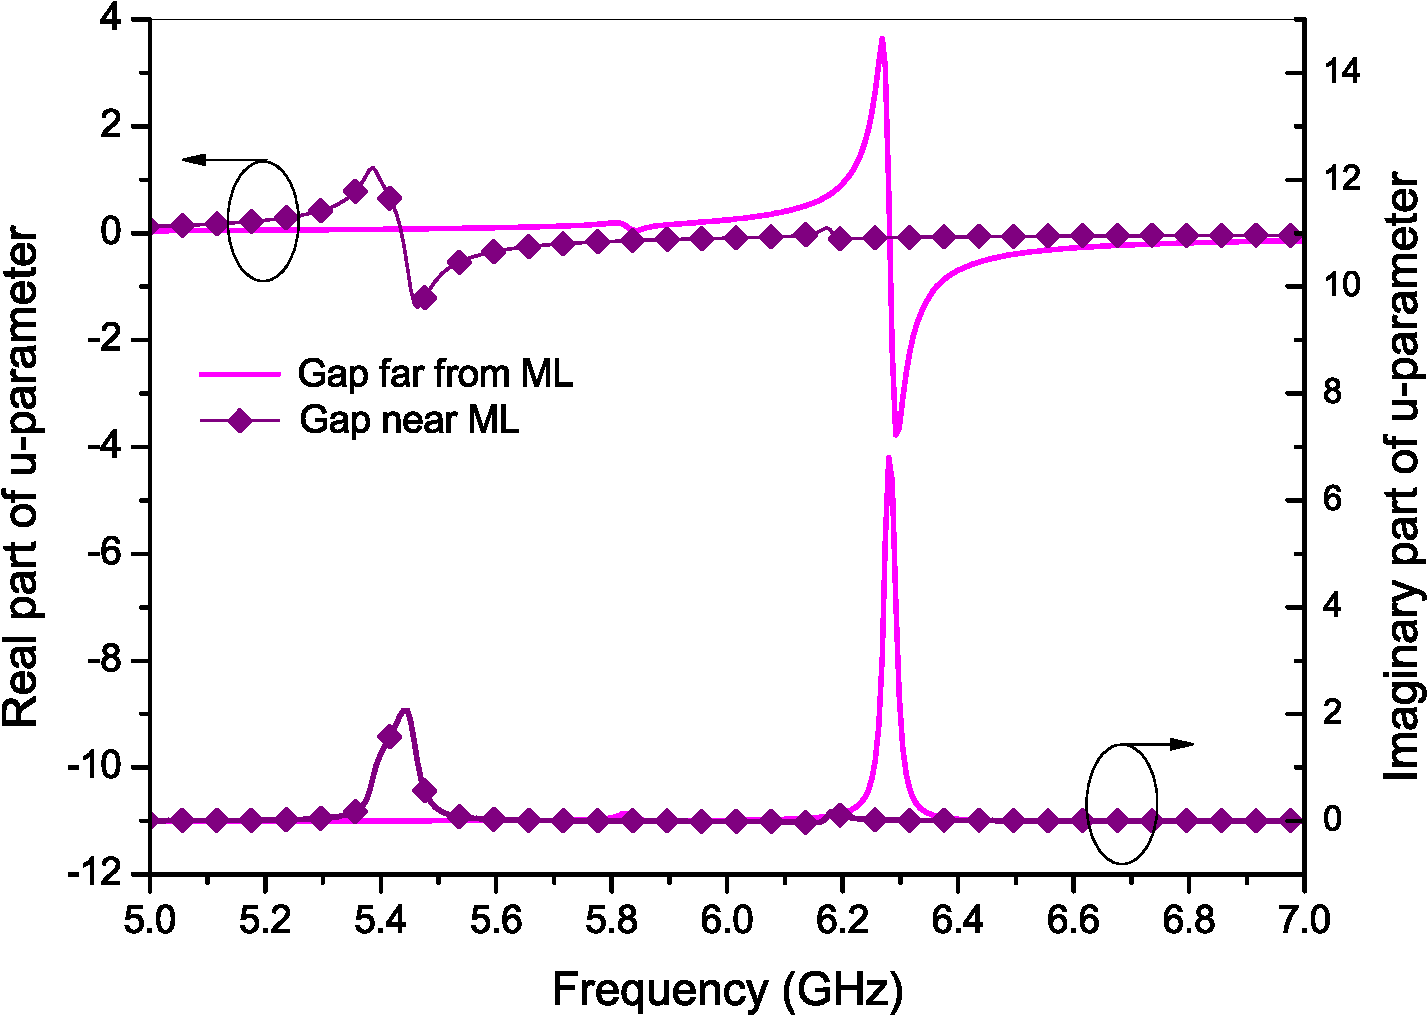
\includegraphics[width=0.6\textwidth]{slike/12a.pdf}
\label{fig12a}}\hfill
\subfloat[]{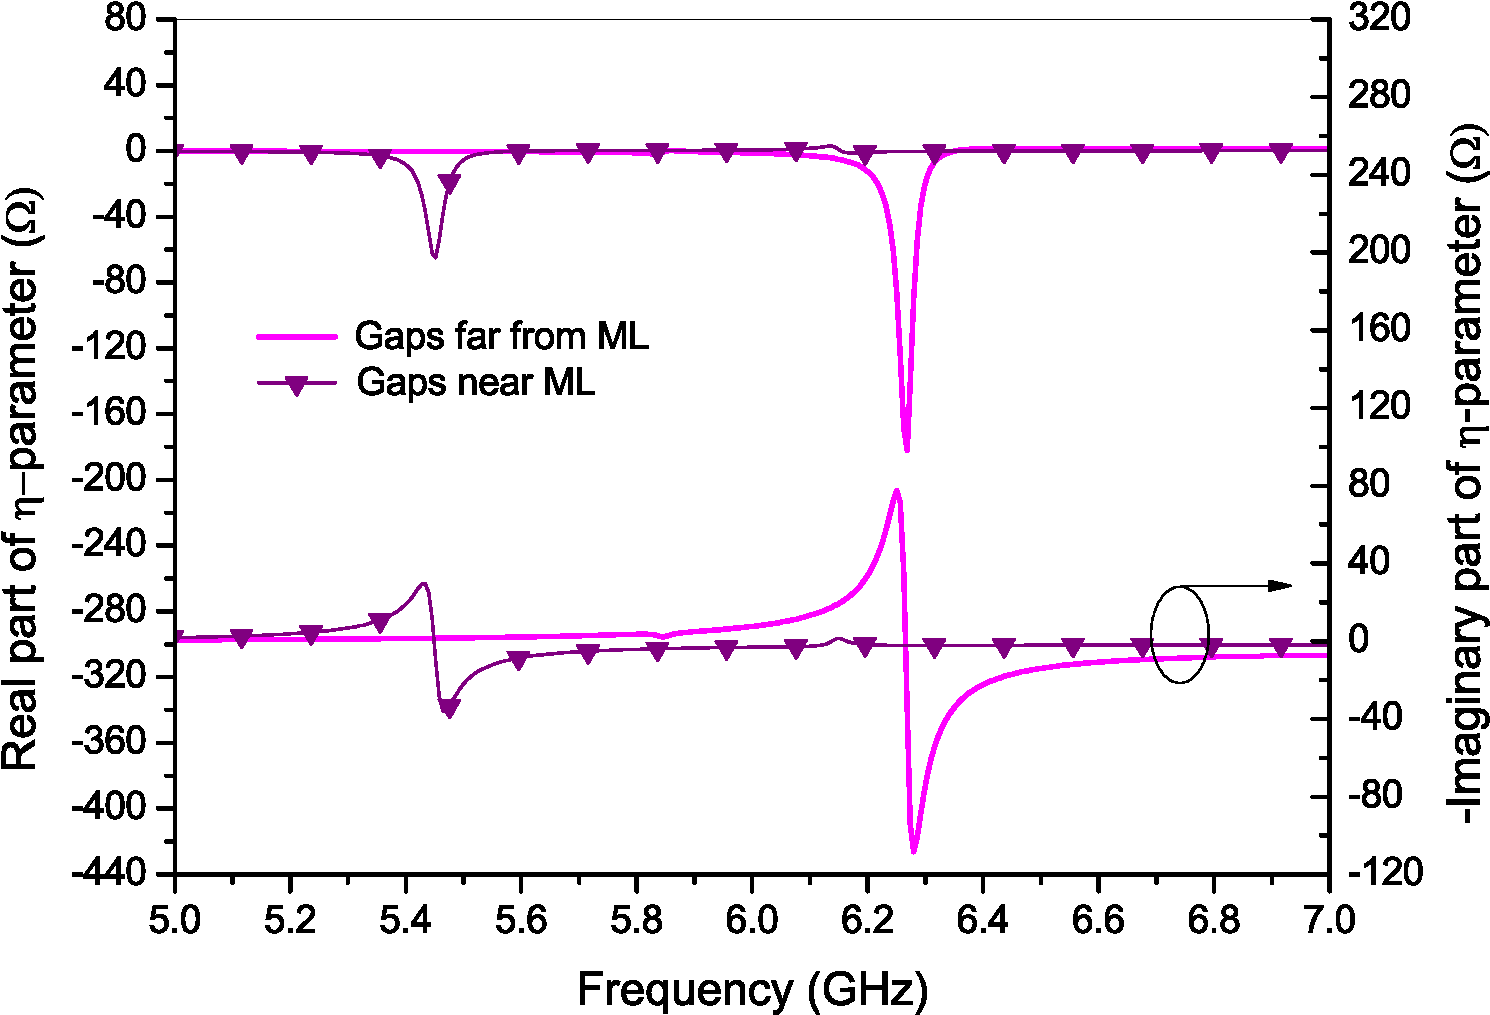
\includegraphics[width=0.6\textwidth]{slike/12b.pdf}
\label{fig12b}}
\caption{Поређење екстрахованих параметара: (а) параметар бианизотропије $u$ и (б) разлика ефективних карактеристичних импеданси, $\eta$, за ћелије са процепом паралелним воду.}
\label{fig12}
\end{figure} 

На сл.~\ref{usl_par} упоређени су стандардни услов за негативни индекс преламања (\ref{usl_std}), који је валидан за симетричне ћелије, и последично за параметре добијене $НРВ_{ср}$ методом, и нови услов (\ref{usln}), који је изведен за асиметричне ћелије. Оба услова су израчуната помоћу параметара добијених ГП методом. У случају ћелија са паралелним процепом даље од вода, види се да су око прве резонансе обе криве преклопљене, јер је одзив симетричан у том опсегу. Око друге резонансе крива која одговара новом услову пресеца $x$-осу тачно на тачкама где је реални део индекса једнак нули, што није случај за криву која одговара стандардном критеријуму. У овом случају, стандардни критеријум предвиђа нешто шири опсег негативног индекса. На крају, применили смо стандардни услов на параметре добијене $НРВ_{ср}$ методом, и показује се да се добијена крива у потпуности преклапа са новим условом. Ово потврђује валидност новог услова, пошто оба метода дају исти индекс преламања, како у симетричном тако и у асиметричном случају.
\begin{figure}[!t]
\centering
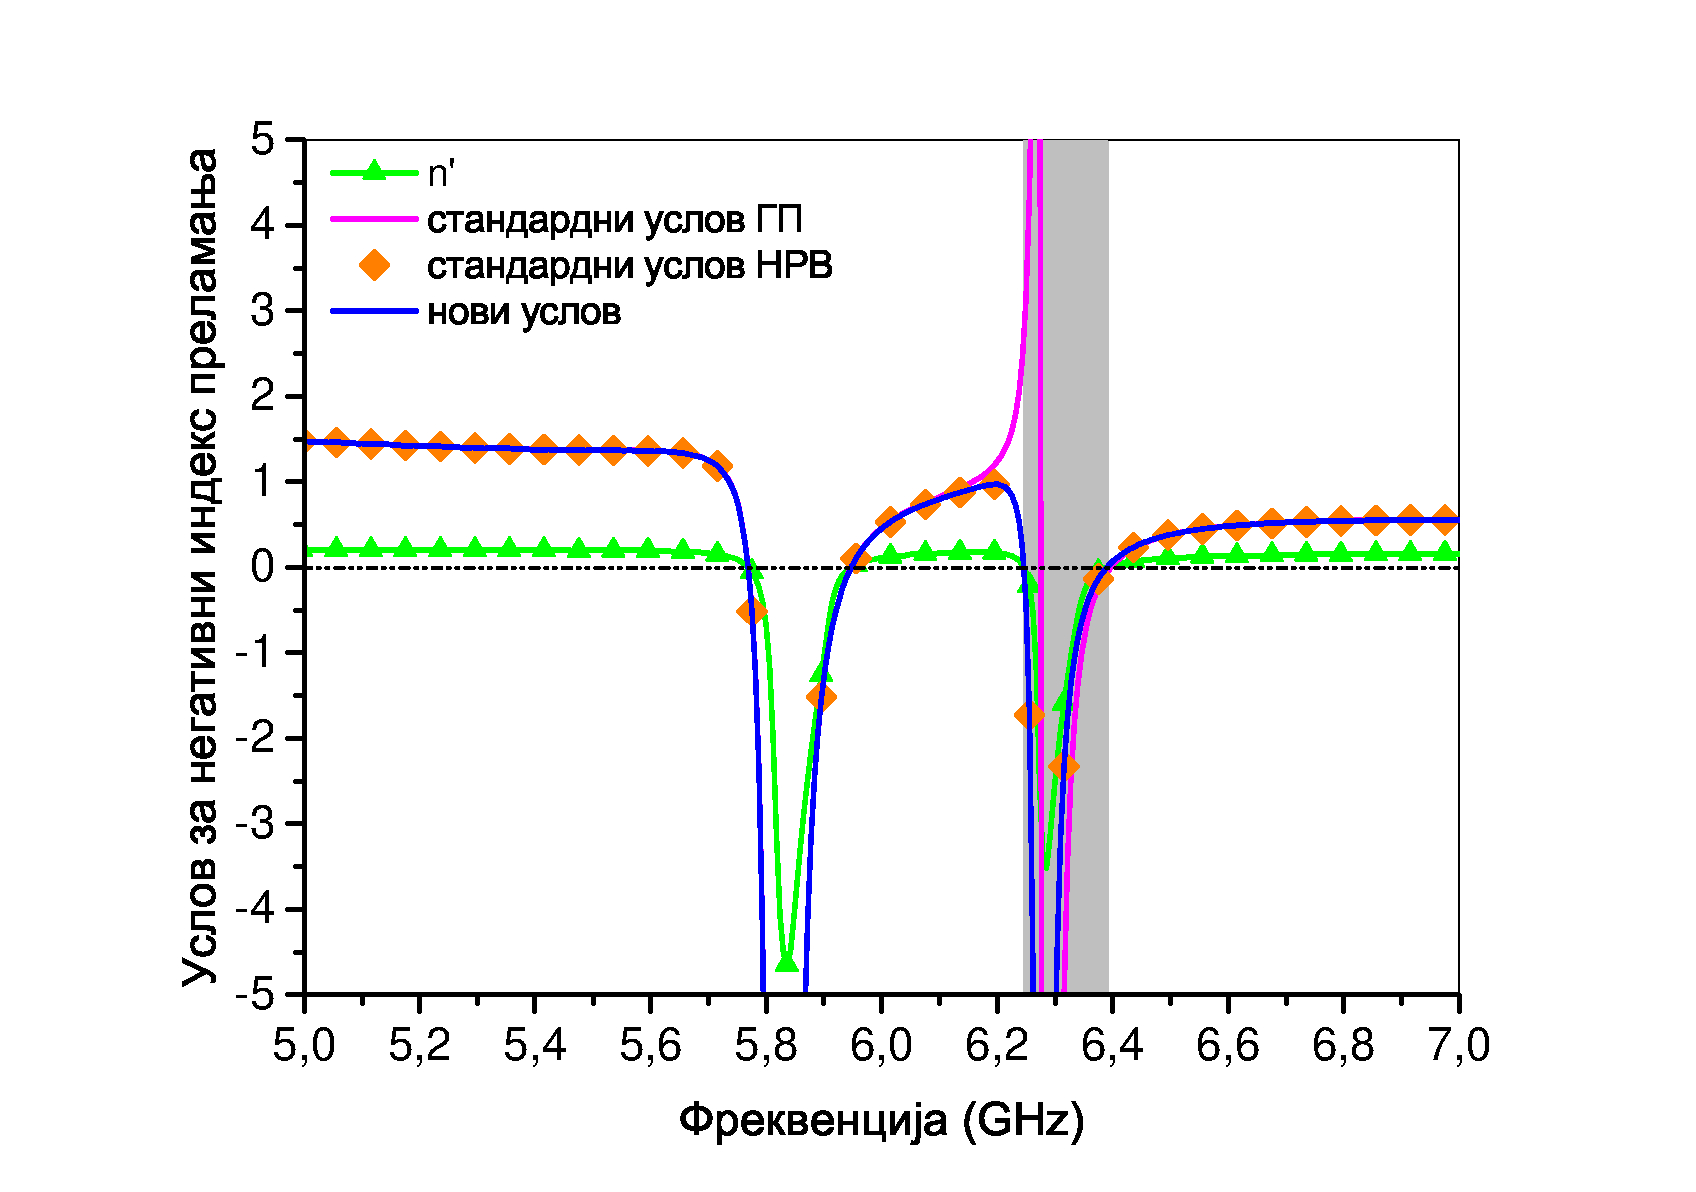
\includegraphics[width=0.6\textwidth]{slike/usl_par.pdf}
\caption{Поређење стандардног и новог критеријума за негативни индекс преламања за јединичну ћелију са процепима паралелним воду. Ефективни параметри су добијени ГП методом. Осенчени правоугаоник означава опсег у коме ћелија има асиметрични одзив и два критеријума предвиђају другачије опсеге негативног индекса.}
\label{usl_par}
\end{figure} 
	
\subsection{Јединичне ћелије са процепима нормалним на вод}

Јединичне ћелије са процепима нормалним у односу на микрострип вод су приказане на сл.~\ref{norm_gep}, и можемо разликовати два случаја у зависности од положаја горњег процепа: а) када је ближе воду и б) даље од њега. У оба случаја процепи су ближе порту 1 јединичне ћелије. Уколико бисмо заменили редослед портова, параметри $u$ и $\eta$ би променили знак, док би све остало било непромењено.
\begin{figure}[!t]
\subfloat[]{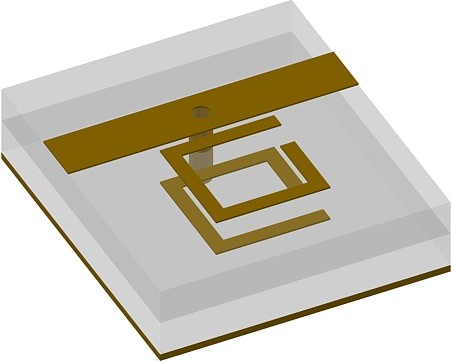
\includegraphics[width=0.45\textwidth]{slike/n1.jpeg}
\label{norm1}}\hfill
\subfloat[]{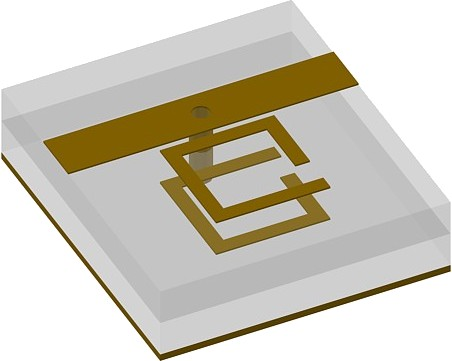
\includegraphics[width=0.45\textwidth]{slike/n2.jpeg}
\label{norm2}}
\caption{Изглед јединичних ћелија које се састоје од АСРР-ова са ивицом која садржи процеп нормалном на вод: (а) горњи процеп ближе воду, (б) горњи процеп даље од вода.}
\label{norm_gep}
\end{figure}

Магнитуда $Ѕ$-параметара за јединичне ћелије са нормалним процепом су приказане на сл.~\ref{fig14_1}. Екстрахована ефективна пермитивност и пермеабилност за случај са горњим процепом ближе и даље од вода су приказане на сл.~\ref{fig14_2}-\ref{fig14_3}, респективно. Може се видети да положај нормалних процепа не утиче на резонантне учестаности у значајној мери. Такође $S_{11}$ се разликује од $S_{22}$ на обе резонансе, али наглашеније на првој. Екстрахована пермитивност и пермеабилност коришћењем ГП и $НРВ_{ср}$ метода се значајно разликују око \SI{5.7}{\giga\hertz} не само по апсолутној вредности, већ имају и супротне знакове.
\begin{figure}[!t]
\centering
\subfloat[]{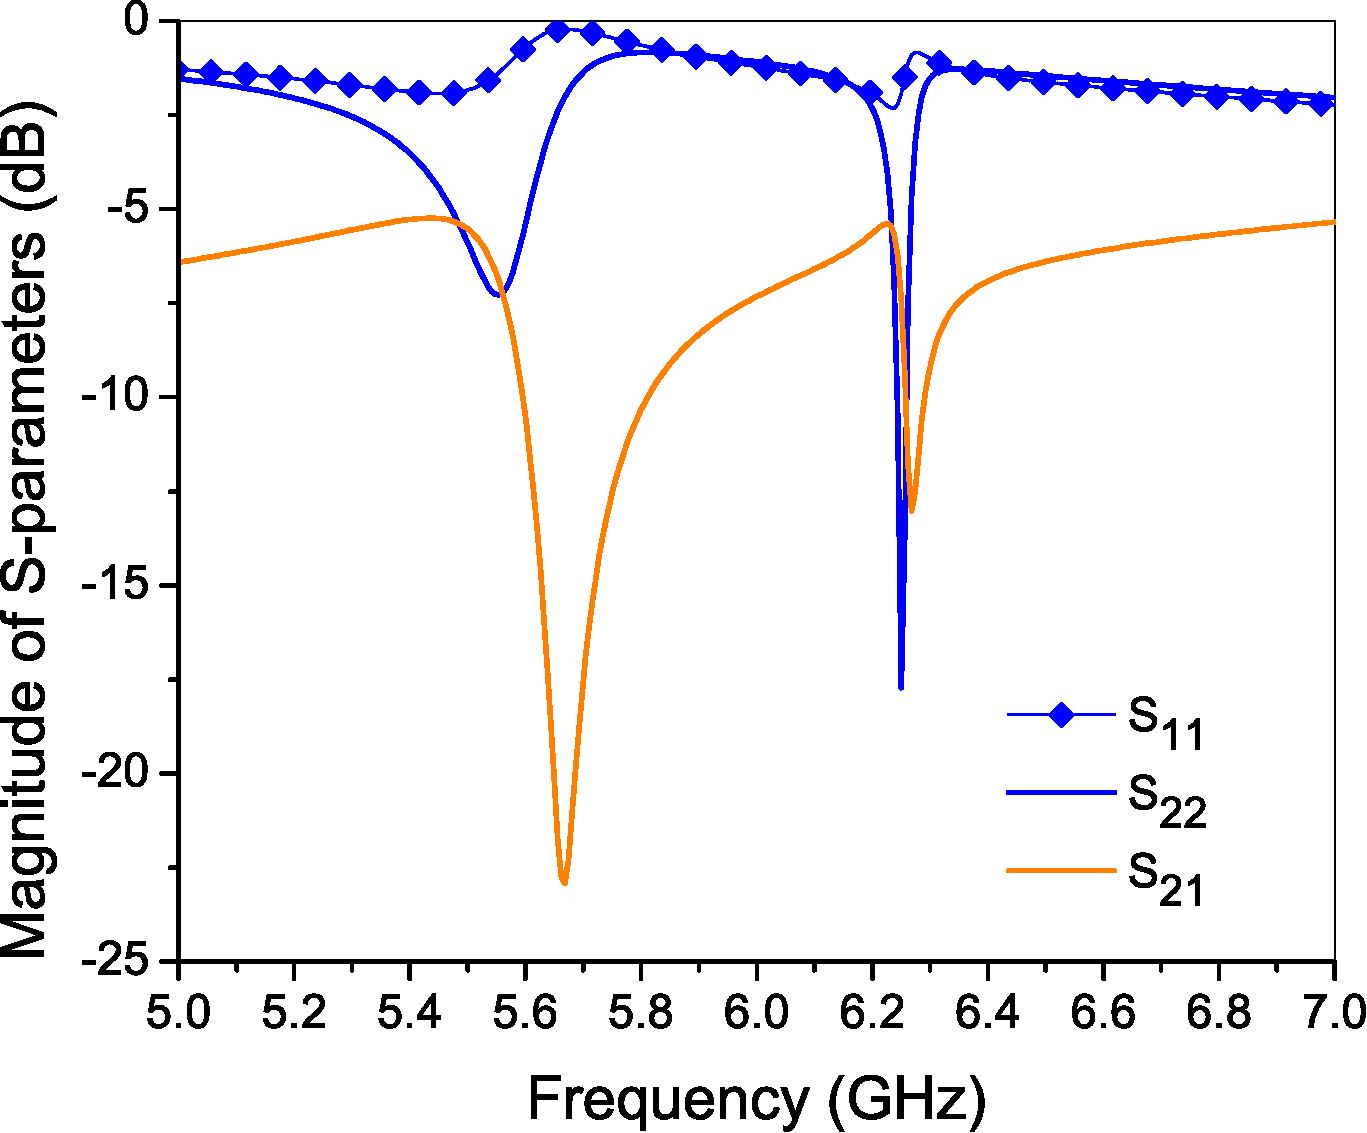
\includegraphics[width=0.45\textwidth]{slike/14a.pdf}
\label{fig14a}}
\hfill
\subfloat[]{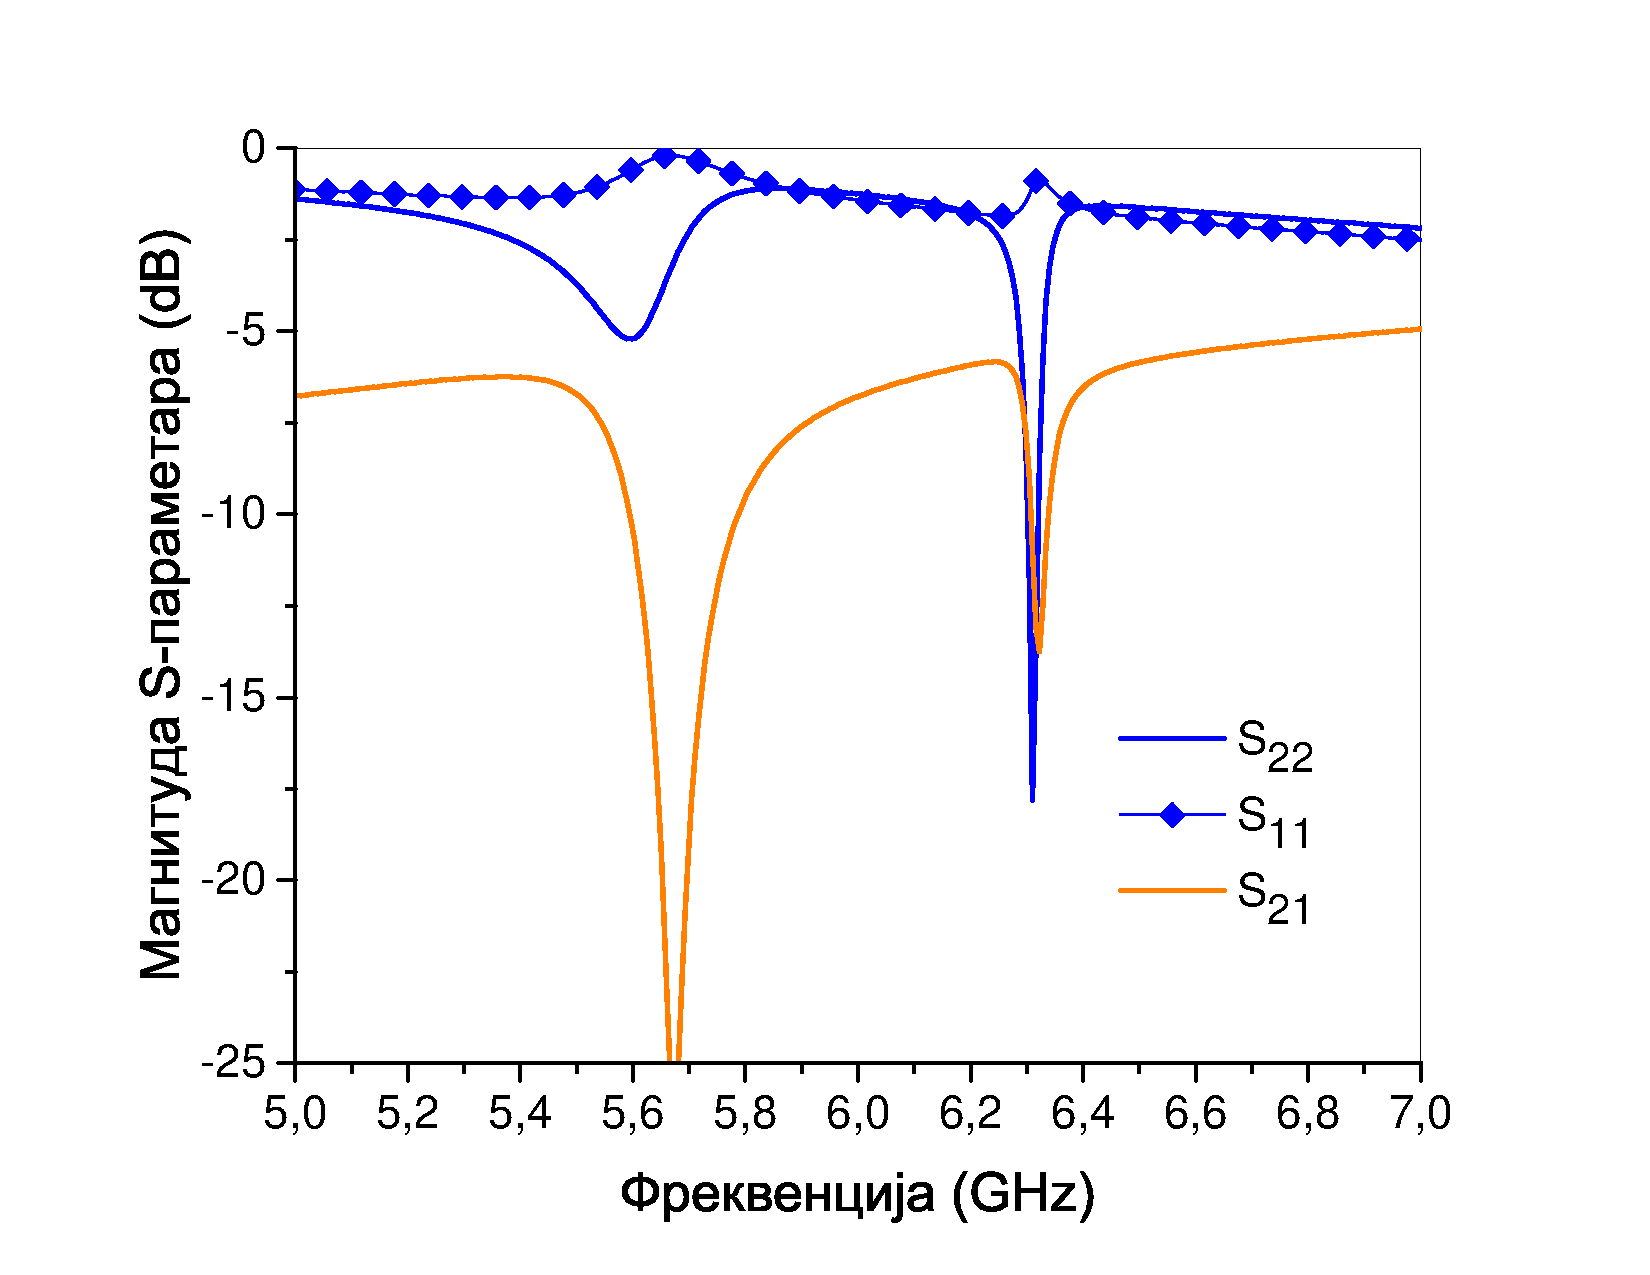
\includegraphics[width=0.45\textwidth]{slike/14b.pdf}
\label{fig14b}}
\caption{Магнитуда $Ѕ$-параметара за јединичне ћелије са нормалним процепом: (а) горњи процеп ближе воду, (б) даље од вода.}
\label{fig14_1}
\end{figure}
\begin{figure}[!t]
\centering
\subfloat[]{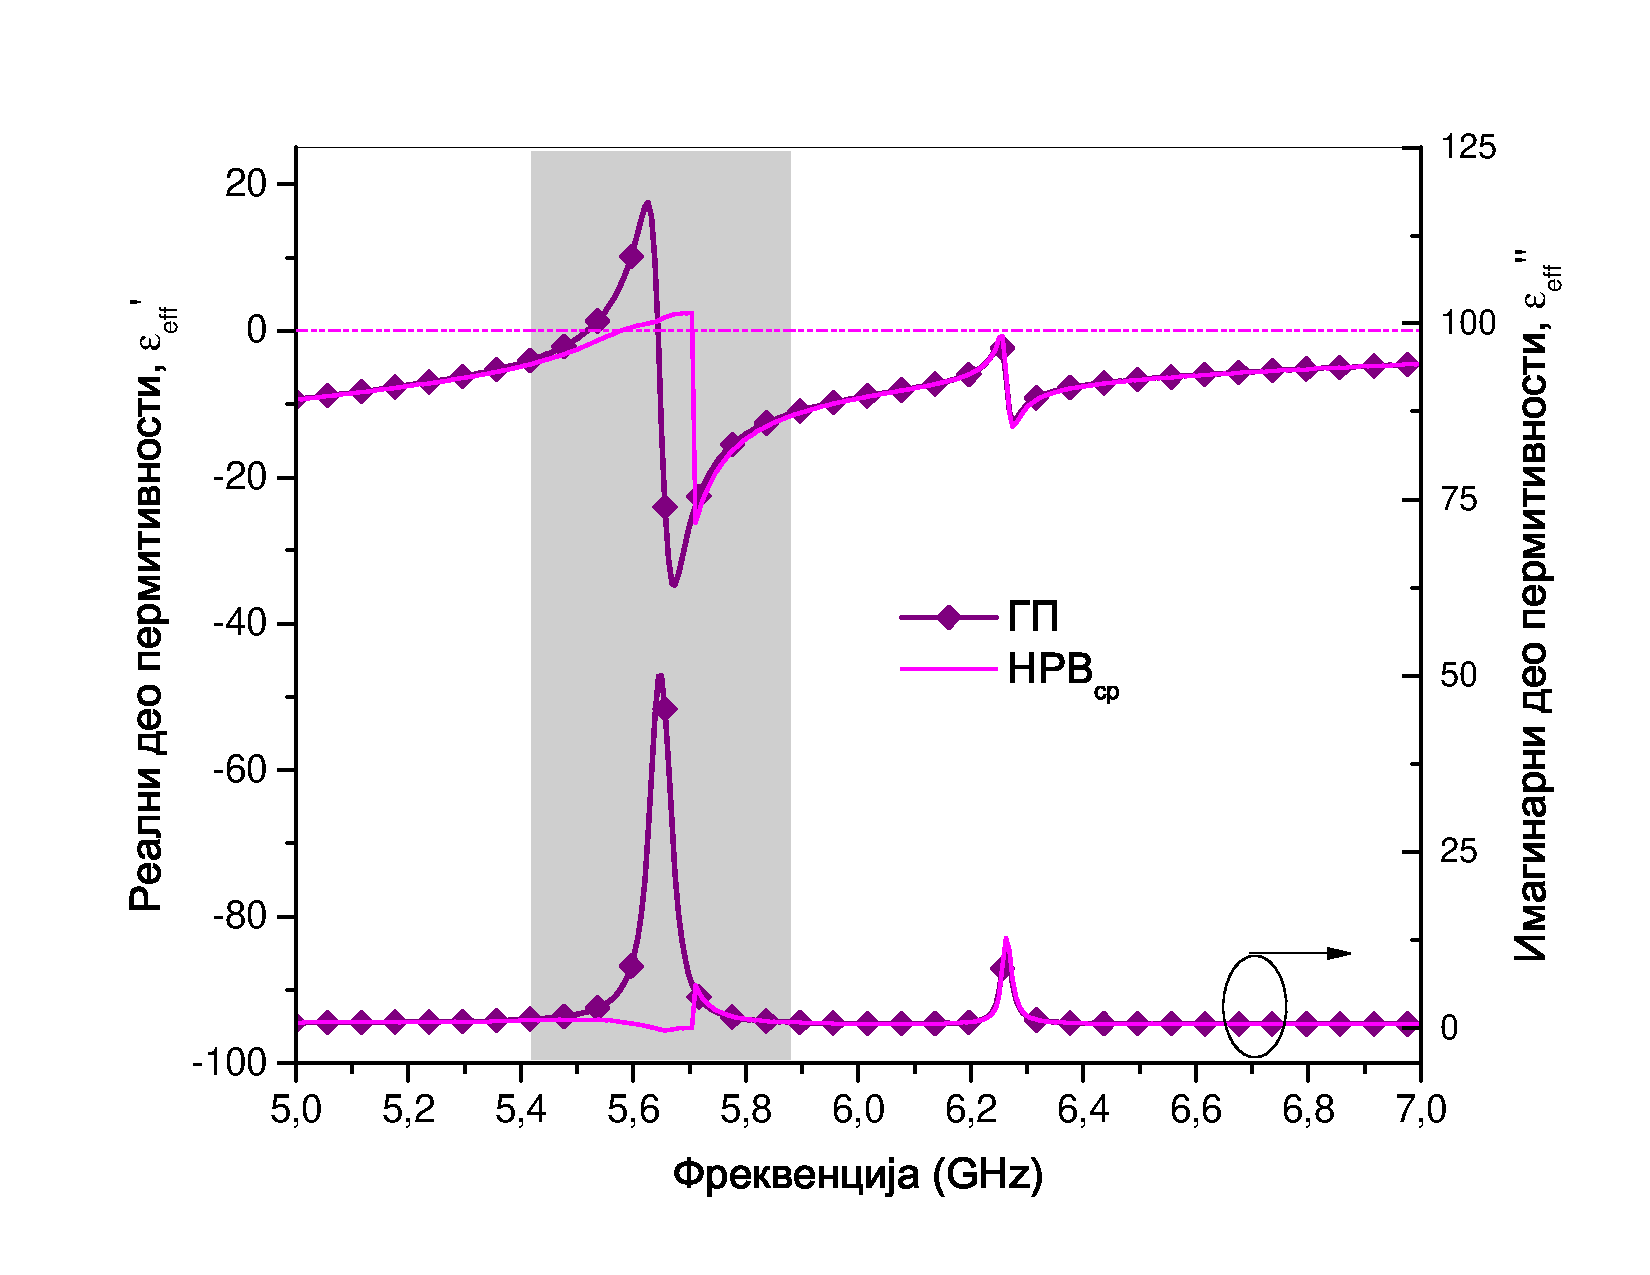
\includegraphics[width=0.5\textwidth]{slike/14c.pdf}
\label{fig14c}}\hfill
\subfloat[]{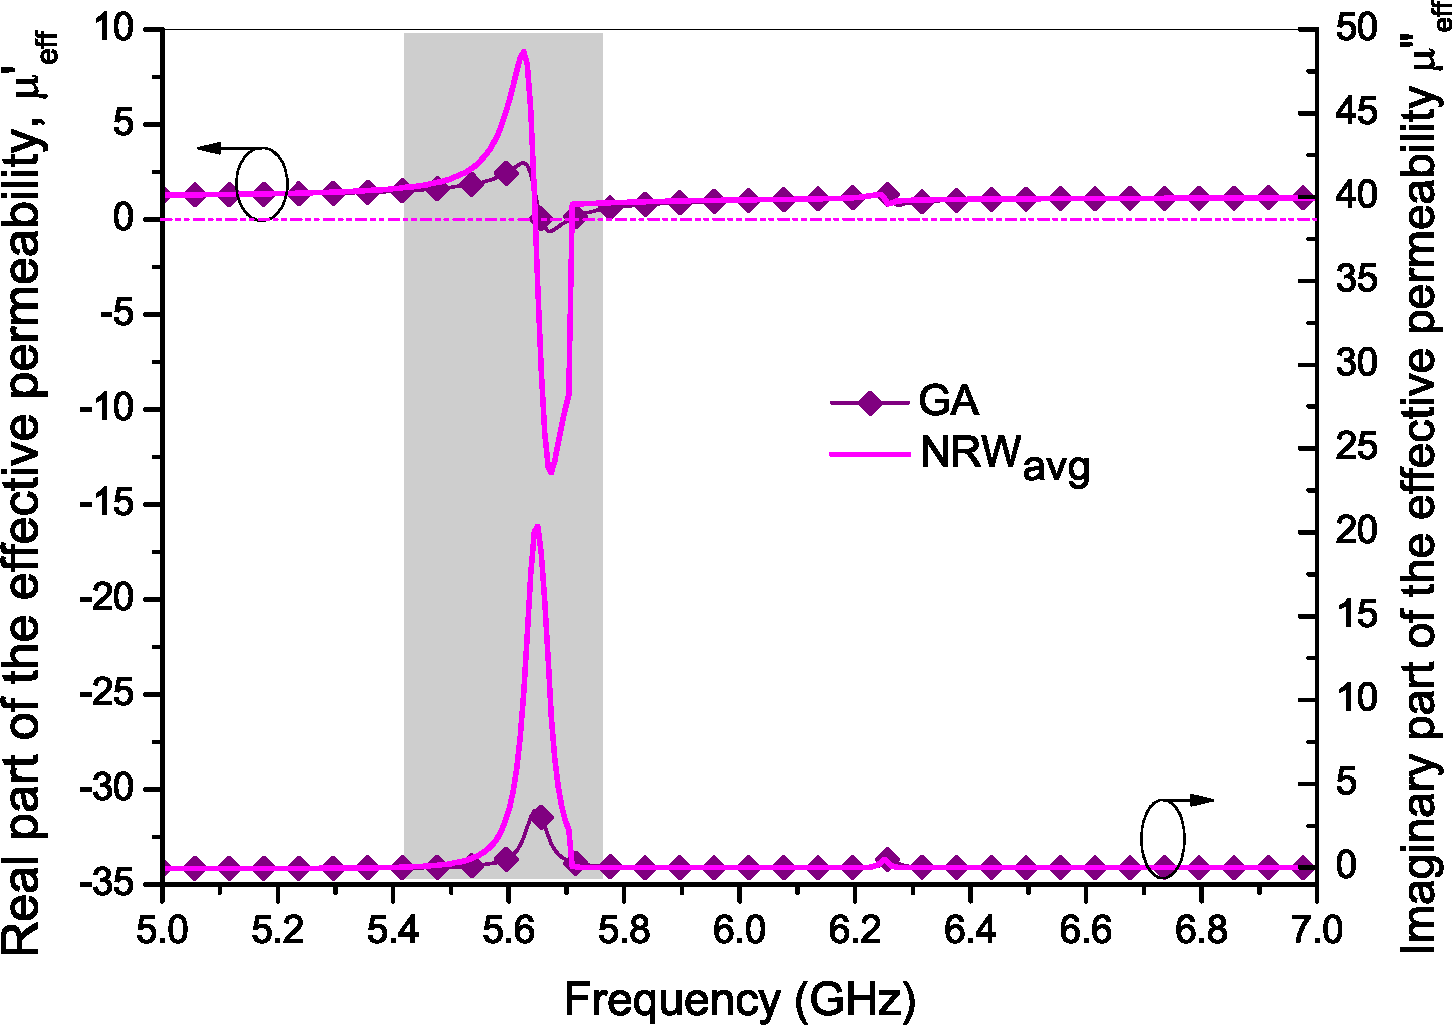
\includegraphics[width=0.5\textwidth]{slike/14e.pdf}
\label{fig14d}}
\caption{Ефективни параметри екстраховани ГП и $НРВ_{ср}$ методама за јединичне ћелије са горњим процепом ближе воду: (а) пермитивност, (б) пермеаблиност. Осенчени правоугаоници означавају зоне у којима две методе дају другачије резултате.}
\label{fig14_2}
\end{figure}
\begin{figure}[!t]
\centering
\subfloat[]{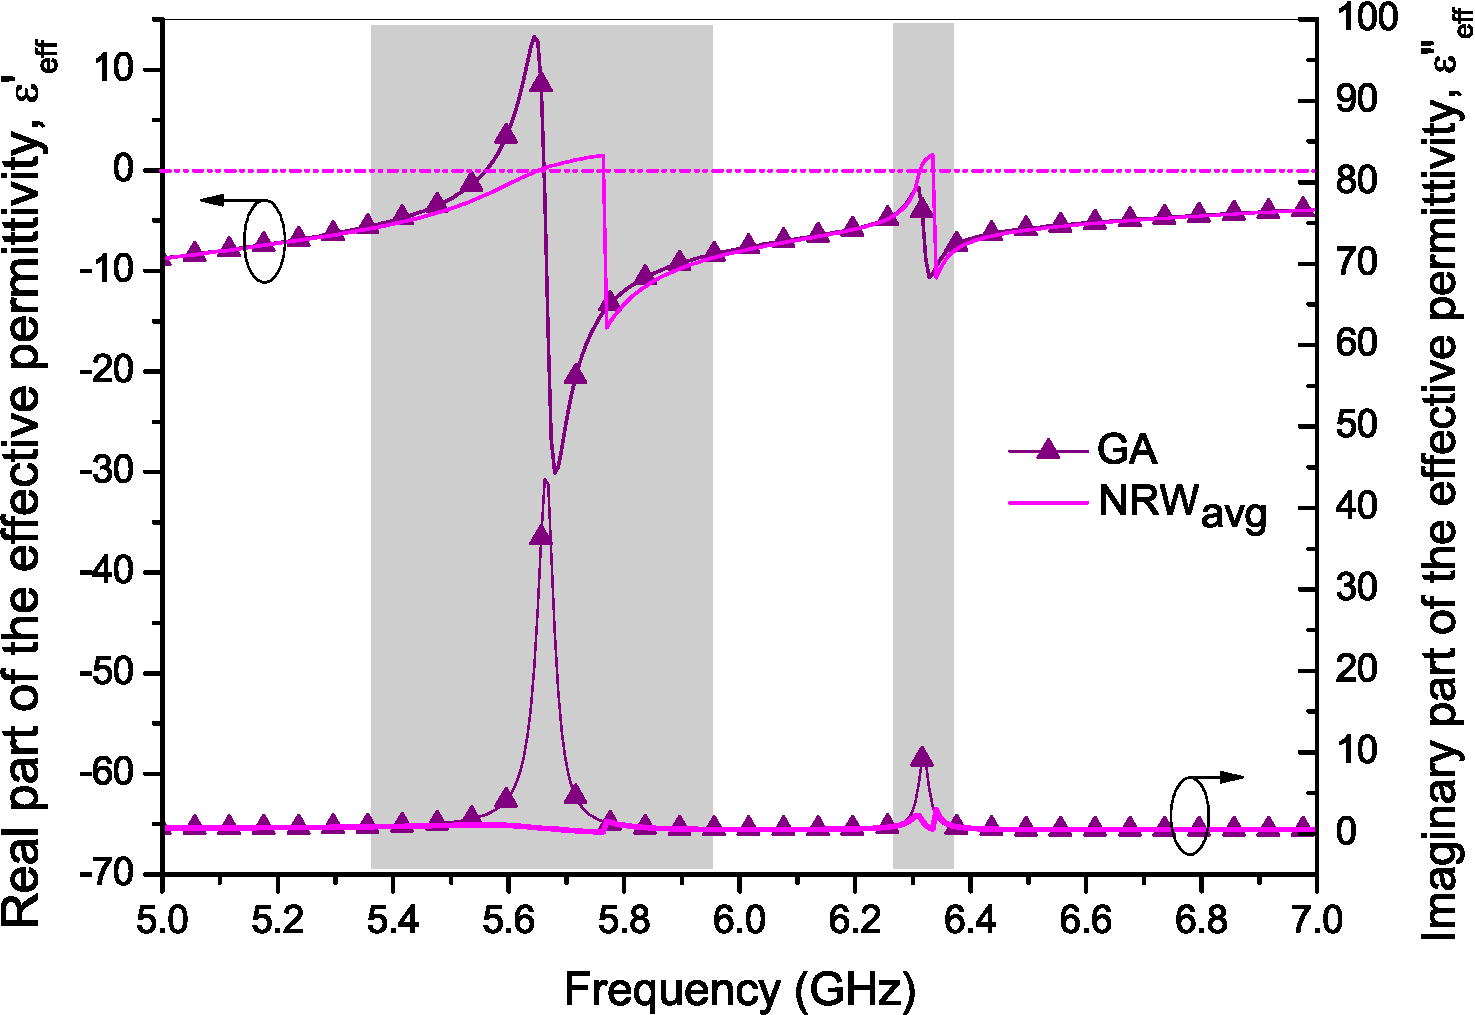
\includegraphics[width=0.6\textwidth]{slike/14d.pdf}
\label{fig14e}}\hfill
\subfloat[]{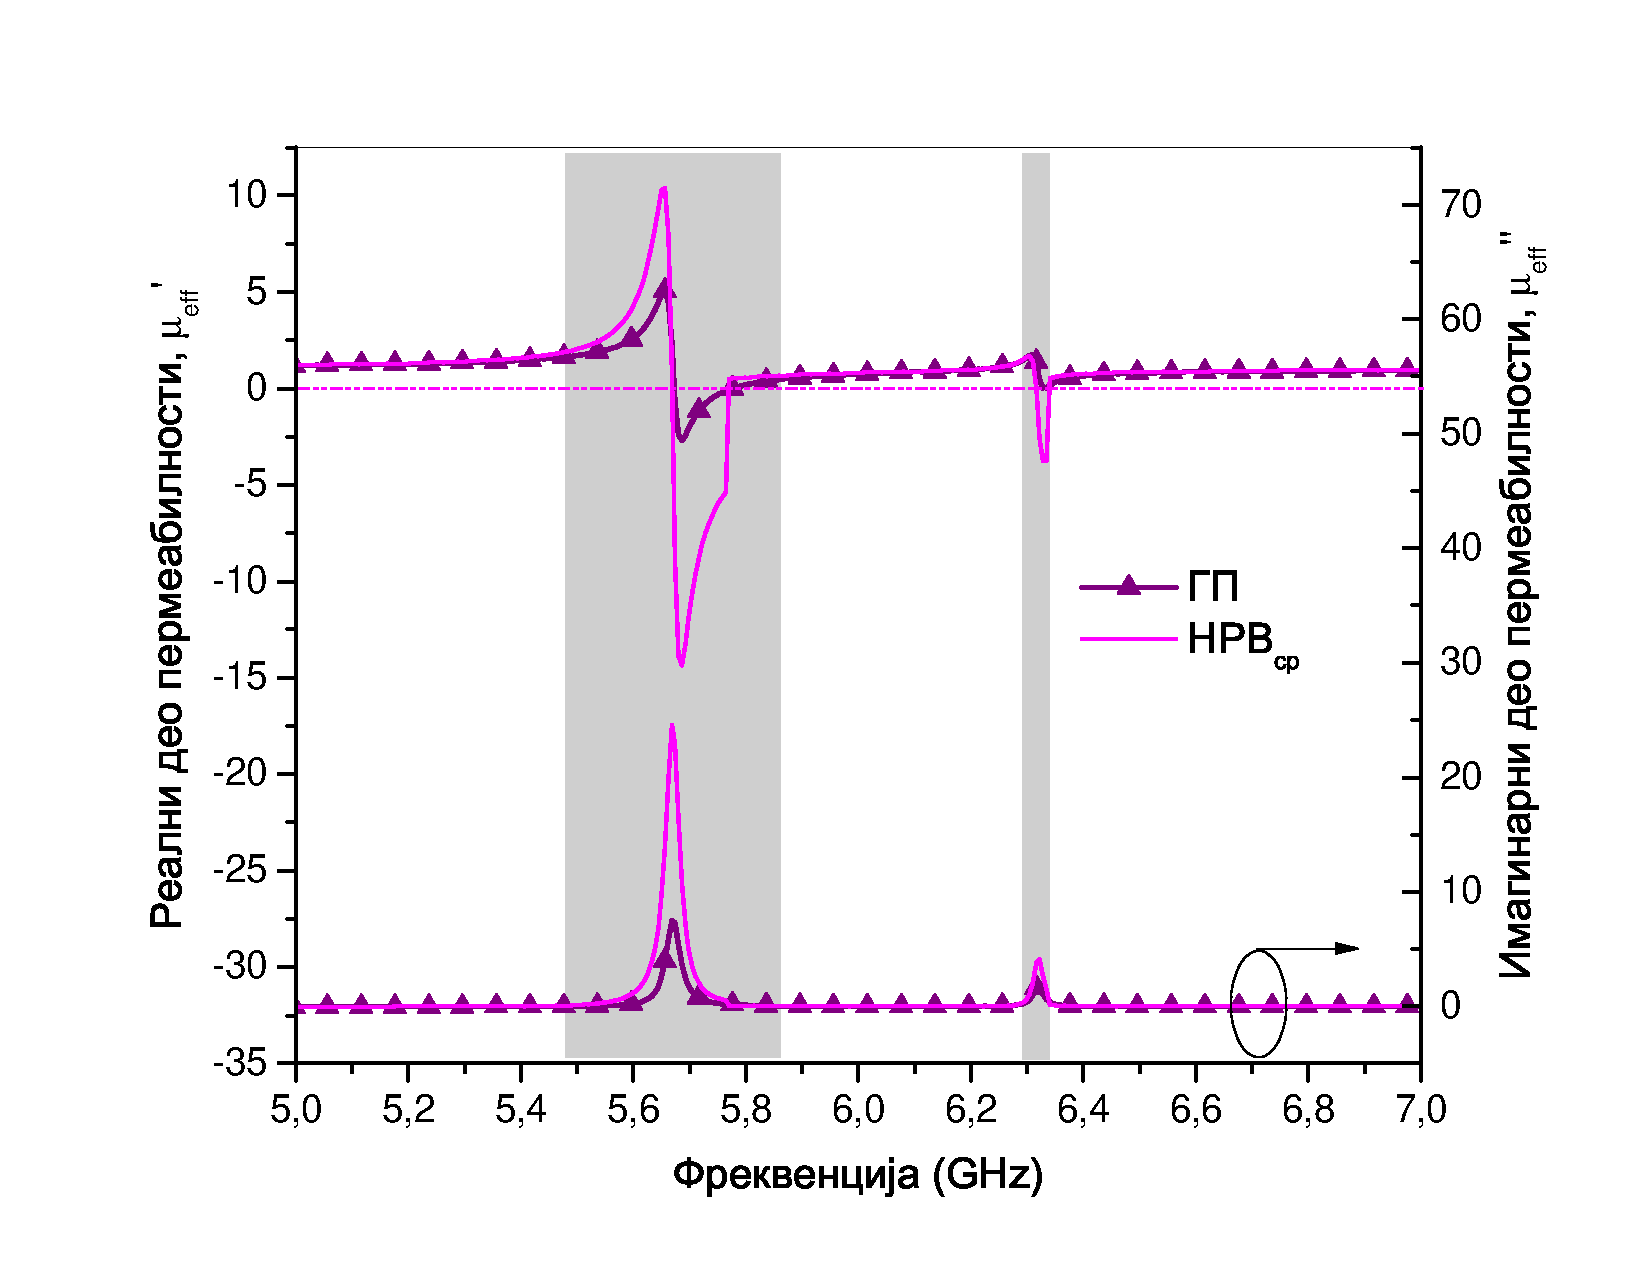
\includegraphics[width=0.6\textwidth]{slike/14f.pdf}
\label{fig14f}}
\caption{Ефективни параметри екстраховани ГП и $НРВ_{ср}$ методама за јединичне ћелије са горњим процепом даље од вода: (а) пермитивност, (б) пермеаблиност. Осенчени правоугаоници означавају зоне у којима две методе дају другачије резултате.}
\label{fig14_3}
\end{figure}

%It can be seen that asymmetry, i.e. difference in $S_{11}$ and $S_{22}$ exist around both resonances. The extracted effective parameters obtained by the two methods differ significantly especially around the first resonance due to the very strong asymmetry. This support our statement that averaged Nicolson-Ross-Weir based on averaging $S_{11}$ and $S_{22}$ is not suitable for highly asymmetric or bianisotropic unit cells.
%
Карактеристике јединичних ћелија са нормалним процепима су упоређене на сл.~\ref{fig15}. Може се видети да је реални део индекса преламања позитиван у целом опсегу за ћелију са процепом ближе воду, док за ћелију са процепом даље од вода поседује уски опсег са негативном вредношћу. Асиметрија је такође много израженија када је процеп даље од вода, као што је био случај и код ћелија са паралелним процепима. Код обе ћелије са нормалним процепима, максимална вредност параметра $u$ ($u_{даље}=\num{8.6}$ и $u_{ближе}=\num{6.6}$) је знатно већа него у случају са паралелним процепима ($u_{даље}=\num{3.69}$ and $u_{ближе}=\num{1.21}$).
\begin{figure}[!t]
\centering
\subfloat[]{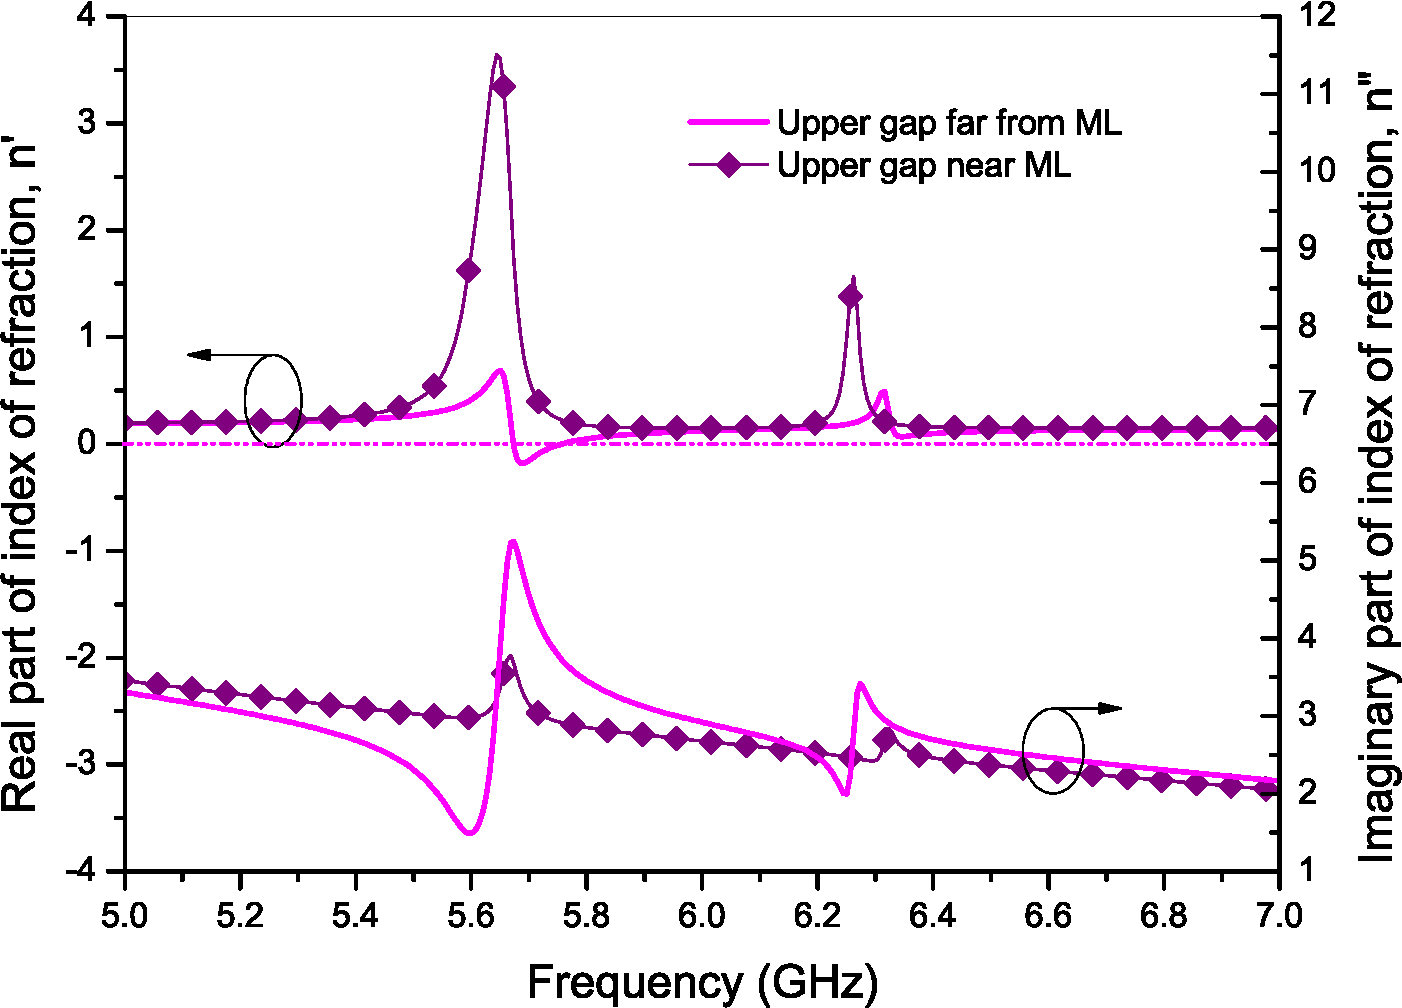
\includegraphics[width=0.6\textwidth]{slike/15a.pdf}
\label{fig15a}}
\subfloat[]{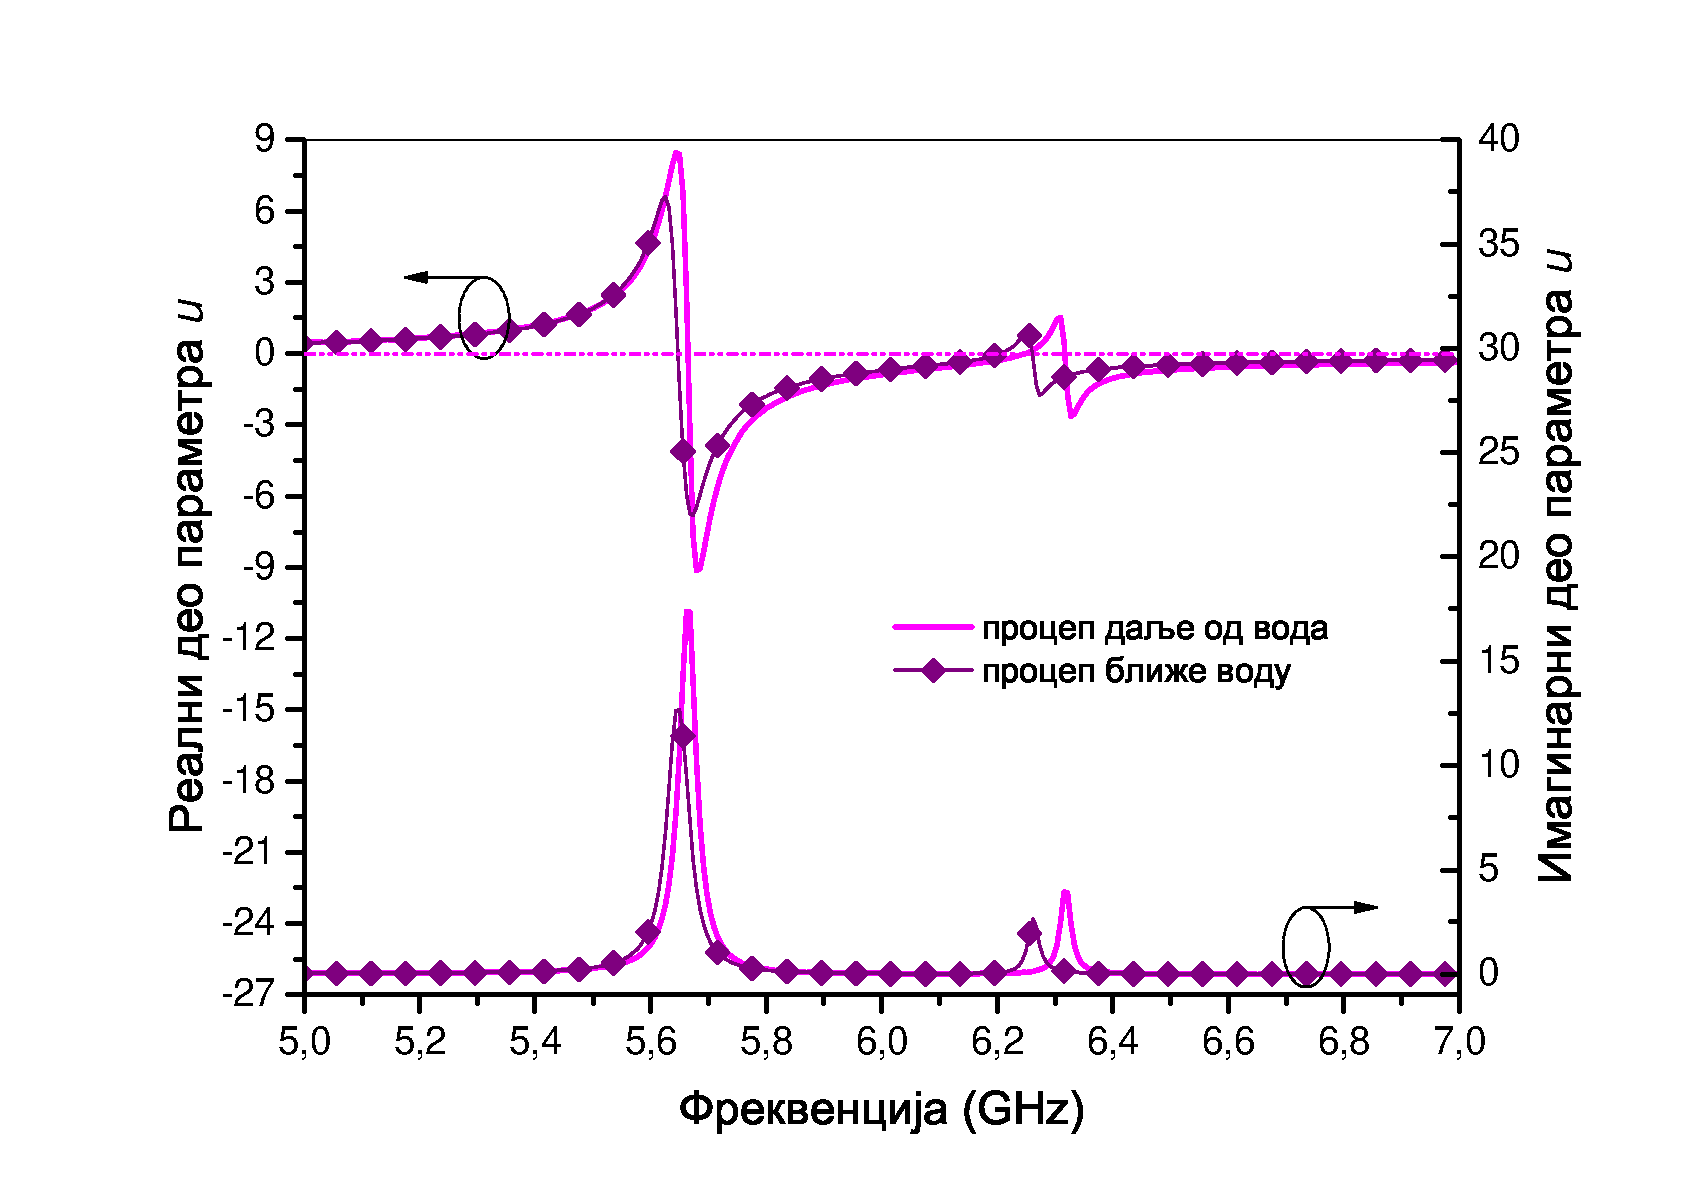
\includegraphics[width=0.6\textwidth]{slike/15b.pdf}
\label{fig15b}}

\caption{Екстраховани индекс преламања (а) и параметар $u$ (б) за јединичне ћелије са нормалним процепима.}
\label{fig15}
\end{figure}

На сл.~\ref{usl_norm} упоређени су стандардни услов за негативни индекс преламања и нови услов, за ћелије са горњим процепом даље од вода. За рачунање оба услова коришћени су параметри добијени ГП поступком. Може се видети да се, око прве резонансе, нови критеријум тачно поклапа са тачкама где реални део индекса пролази кроз нулу. То није случај са стандардним критеријумом, који предвиђа осетно већи опсег негативних вредност индекса. Око друге резонансе на \SI{6.3}{\giga\hertz} стандардни критеријум предвиђа негативне вредности, док је индекс заправо позитиван. Као доказ валидности новог критеријума додата је криву која одговара стандардном критеријуму, али срачунатом за параметре добијене $НРВ_{ср}$ методом, која се у потпуности поклапа са новим критеријумом.
\begin{figure}[!t]
\centering
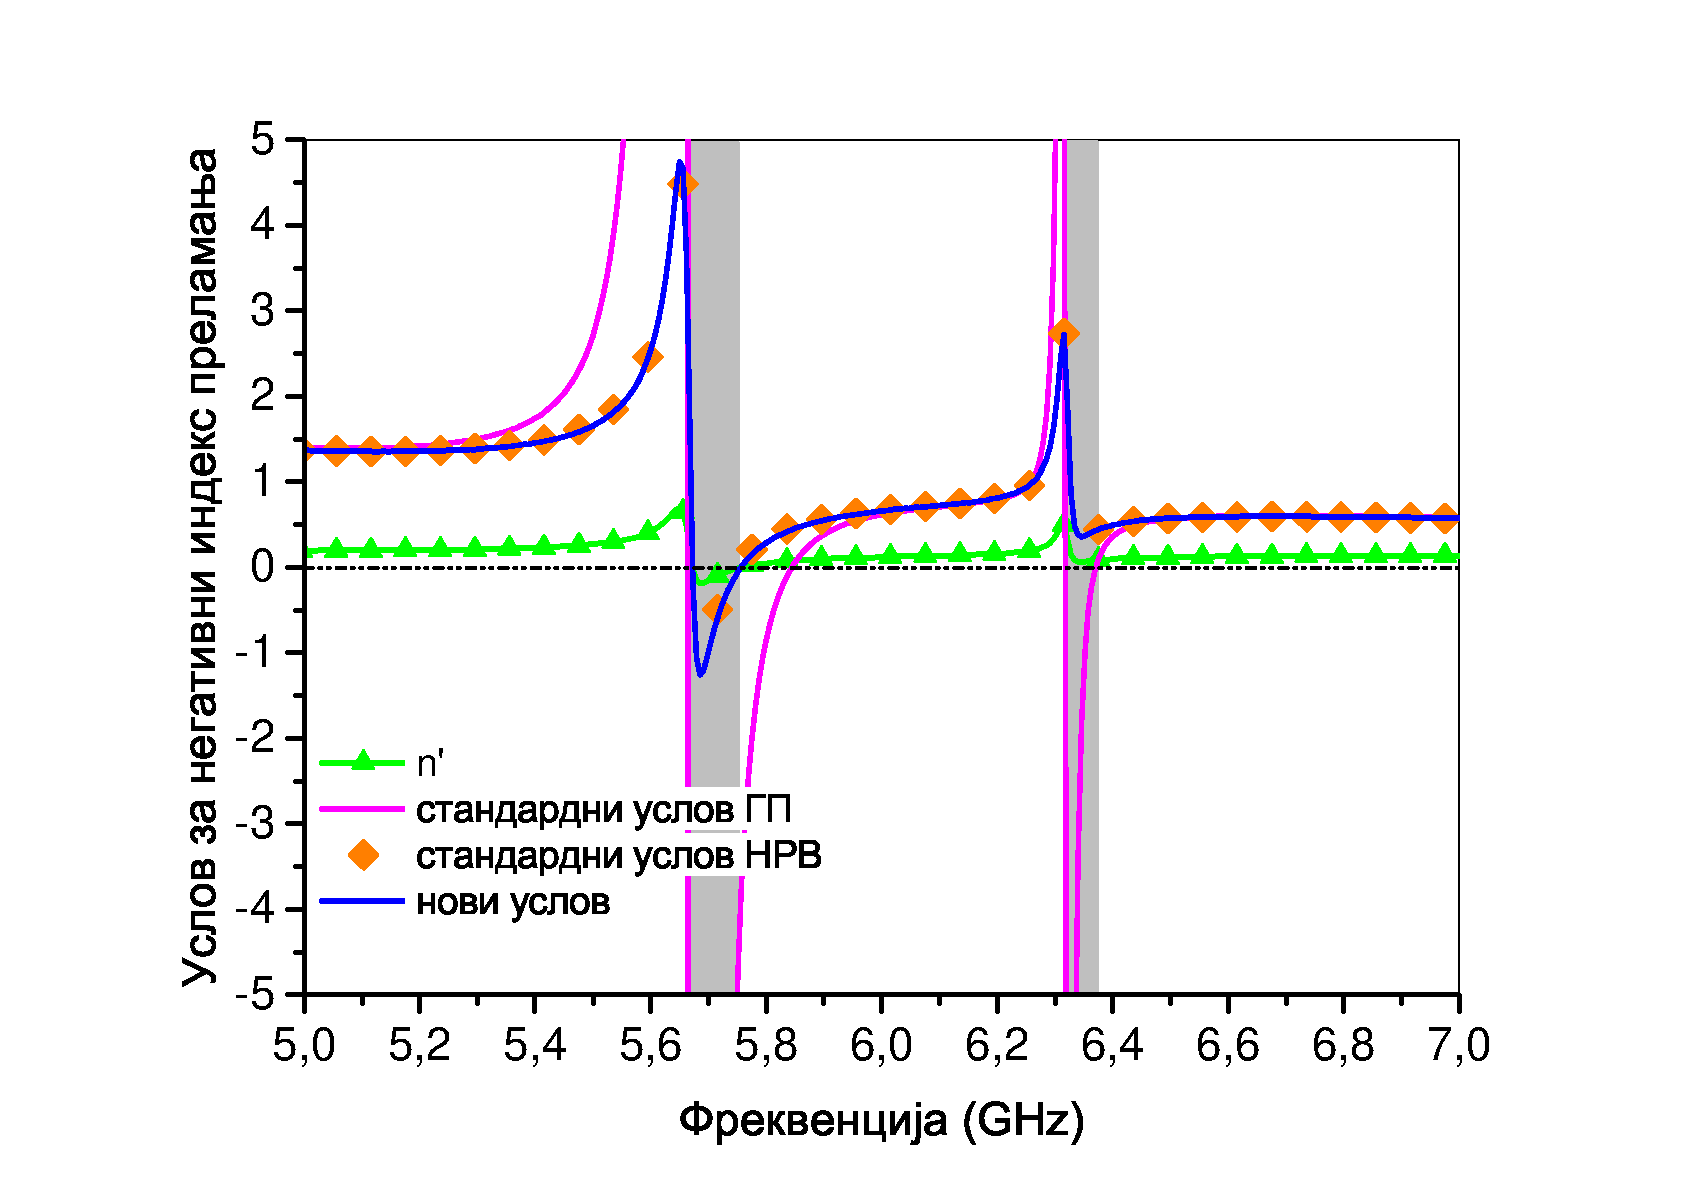
\includegraphics[scale=\SkalaC]{slike/usl_norm.pdf}
\caption{Поређење стандардног и новог критеријума за негативни индекс преламања, за ћелију са нормалним процепом даље од вода. Осенчене су зоне где ћелија има асиметрични одзив и два критеријума предвиђају различите опсеге негативних вредности.}
\label{usl_norm}
\end{figure}

\subsection{Ивично спрегнути СРР}% (\emph{физ.скрипта})}

\newcommand{\labelaslike}{а)~СРР са паралелним процепима, б)~СРР са нормалним процепима. }
%(Такође су разматране)
На сл.~\ref{ph:fig1} приказане су структуре, са релевантним димензијама, код којих су коришћени ивично спрегнути (\foreign{edge-coupled}) СРР-ови. Код њих су прстенови постављени концентрично у истој равни, што знатно олакшава фабрикацију, пошто нема потребе за двослојним диелектриком. С друге стране, смањена је слобода приликом пројектовања. Поново су присутна два случаја, у зависности од тога да ли су процепи оријентисани паралелно (\ref{ph:fig1a}) или нормално (\ref{ph:fig1b}) у односу на вод.
\begin{figure}[!t]
\centering
\subfloat[]{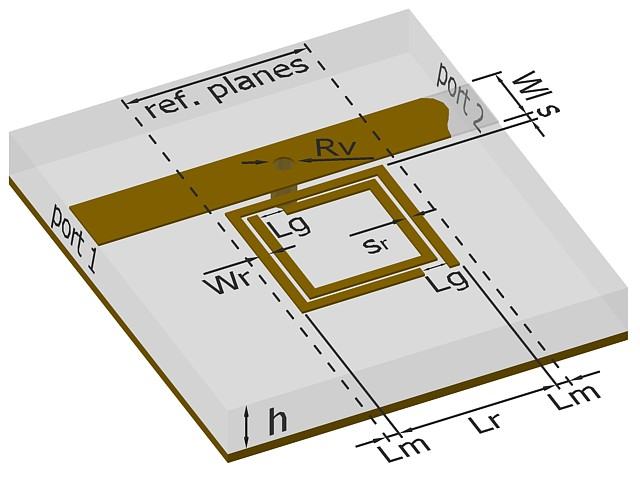
\includegraphics[width=0.45\textwidth]{slike/physcr/pod0/model.jpeg}
\label{ph:fig1a}}
\hfill
\subfloat[]{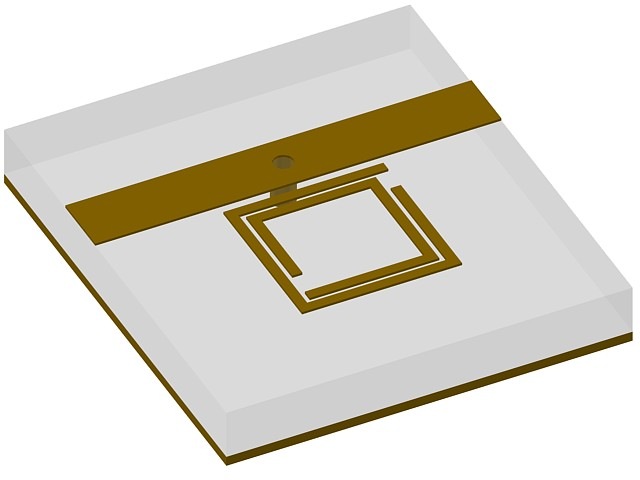
\includegraphics[width=0.45\textwidth]{slike/physcr/pod90/model.jpeg}
\label{ph:fig1b}}
\caption{Ћелије са ивично спрегнутим СРР-овима: \labelaslike Релевантне димензије: $h=\num{1.27}\,\mathrm{mm}$, $L_r=3\,\mathrm{mm}$, $L_g=\num{0.5}\,\mathrm{mm}$, $L_m=\num{0.25}\,\mathrm{mm}$, $W_l=\num{1.2}\,\mathrm{mm}$, $W_r=\num{0.2}\,\mathrm{mm}$, $R_v=\num{0.5}\,\mathrm{mm}$, $s=\num{0.1}\,\mathrm{mm}$, $s_r=\num{0.1}\,\mathrm{mm}$, и релативна пермитивност супстрата $\varepsilon_r=\num{10.2}$.}
\label{ph:fig1}
\end{figure} 

\begin{figure}[!t]
\centering
\subfloat[]{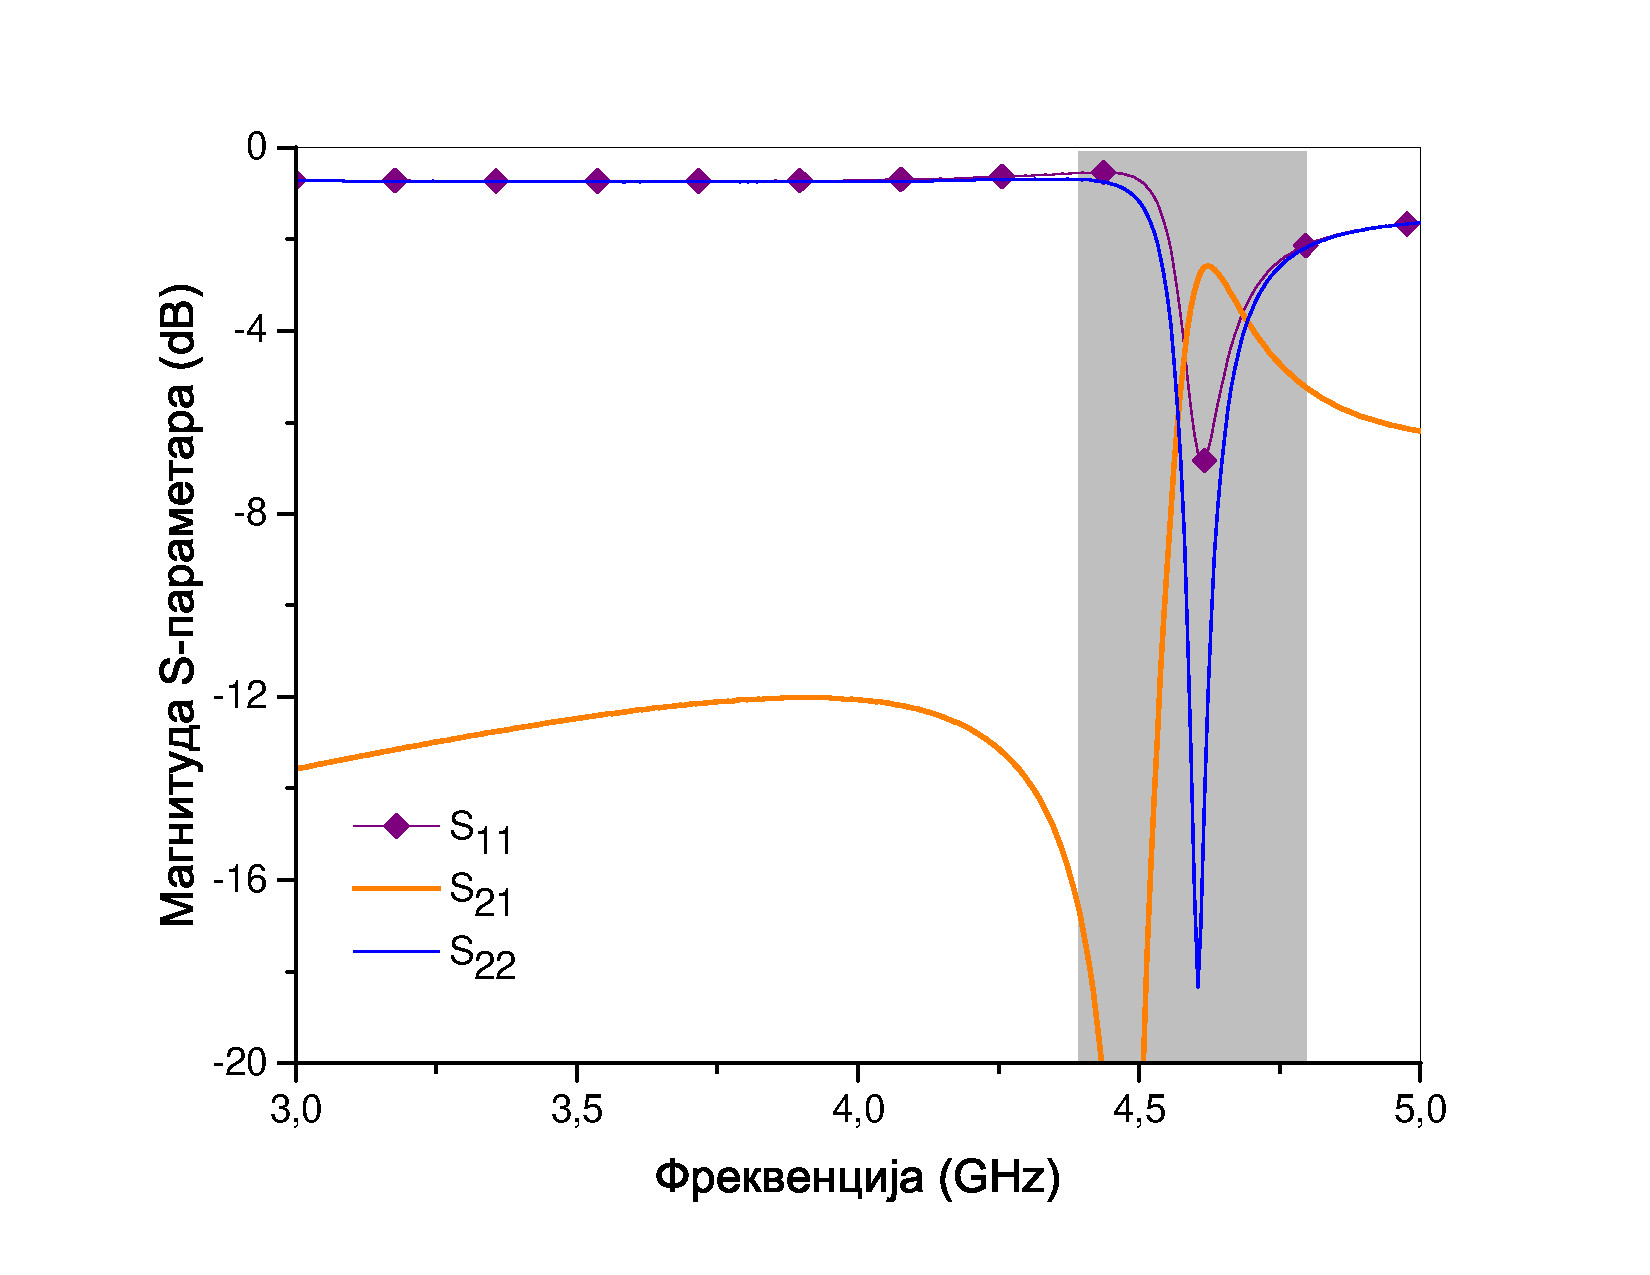
\includegraphics[width=0.48\textwidth]{slike/physcr/pod0/smag}}
%\label{fig}}
\hfill%\hspace*{1cm}
\subfloat[]{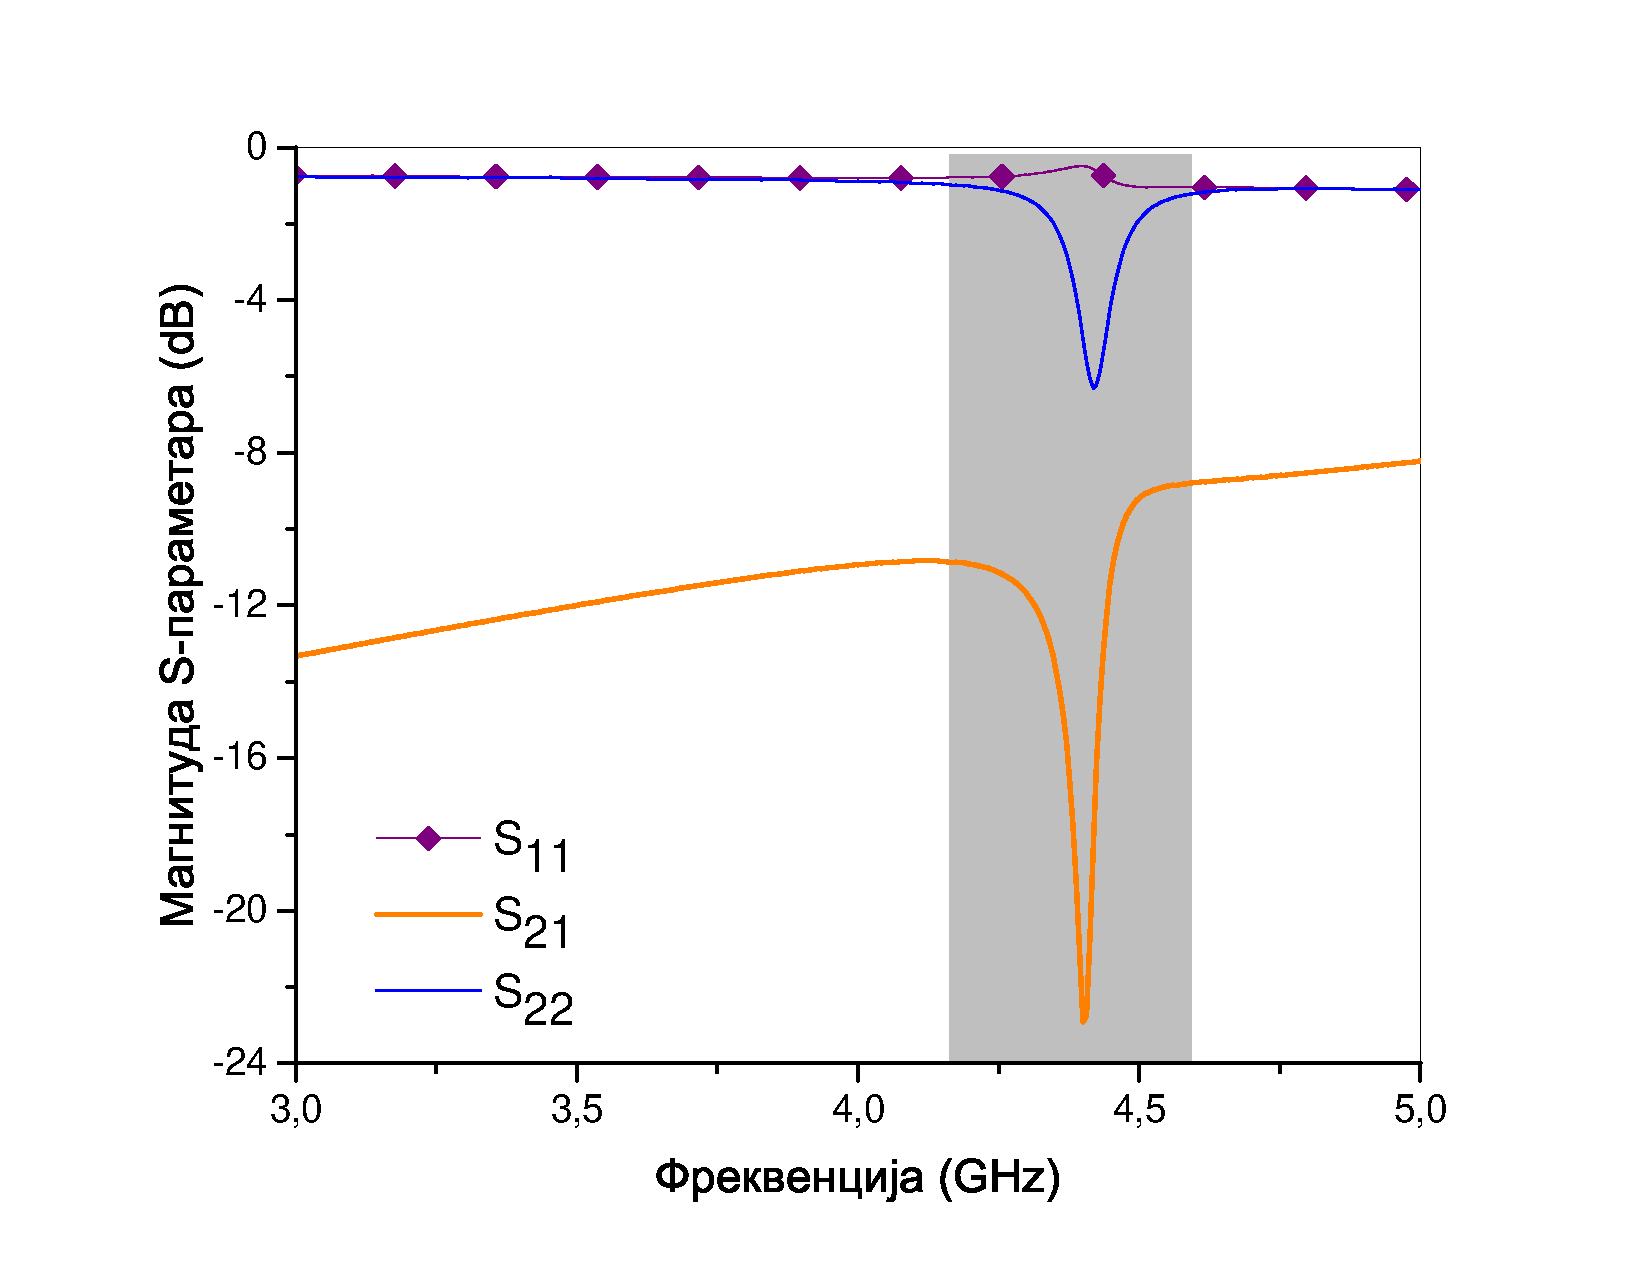
\includegraphics[width=0.48\textwidth]{slike/physcr/pod90/smag}}
%\label{fig}}
\caption{Магнитуда $S$-параметара: \labelaslike Асиметрија је присутна у осенченим деловима.}
\label{ph:fig2}
\end{figure} 

\begin{figure}[!t]
\centering
\subfloat[]{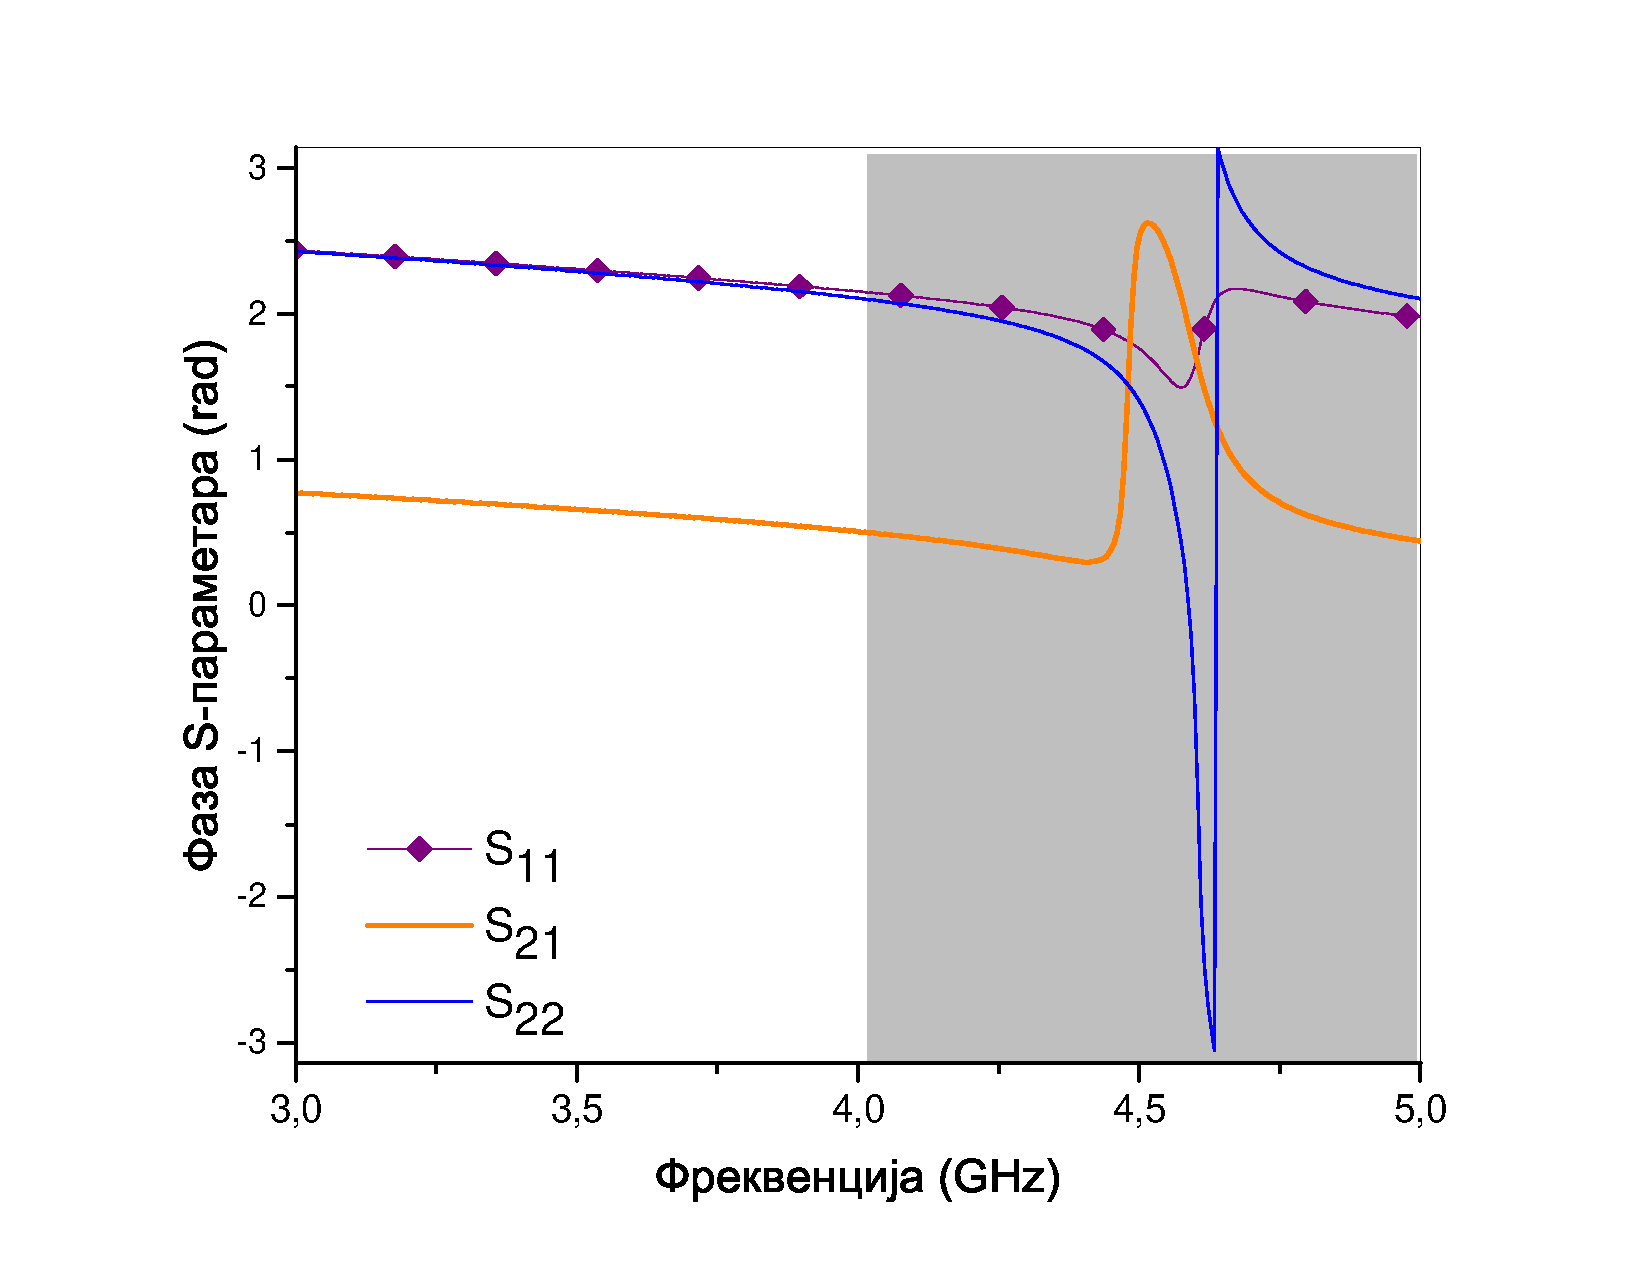
\includegraphics[width=0.48\textwidth]{slike/physcr/pod0/sfaza}}
%\label{fig}}
%\hspace*{1cm}
\subfloat[]{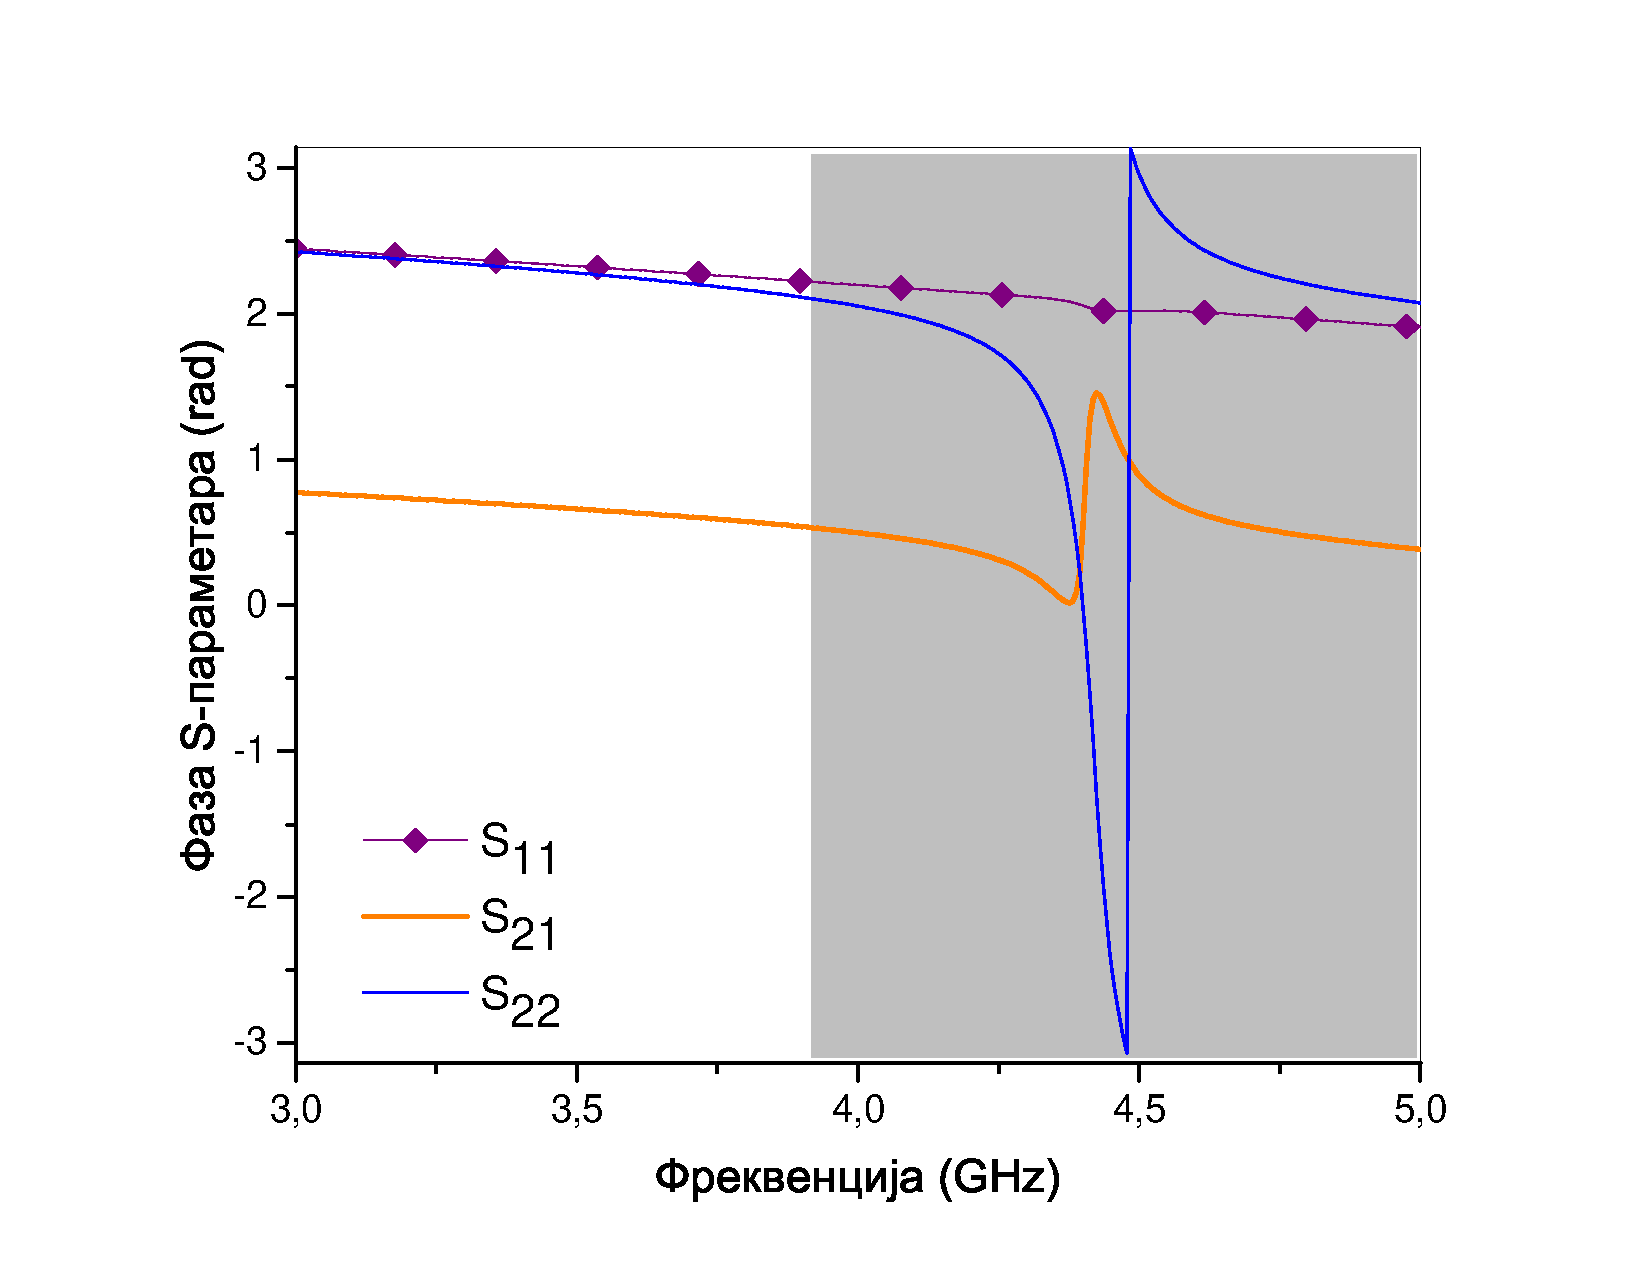
\includegraphics[width=0.48\textwidth]{slike/physcr/pod90/sfaza}}
%\label{fig}}
\caption{Фаза $S$-параметара: \labelaslike Асиметрија је присутна у осенченим деловима.}
\label{ph:fig3}
\end{figure} 
Симулирани $Ѕ$-параметри приказани су на сл.~\ref{ph:fig2}-\ref{ph:fig3}; види се да је асиметрија присутна само око резонанси, при чему је много израженија за случај са нормалним процепима са сл.~\ref{ph:fig1b}. Екстраховани ефективни параметри -- индекс преламања, карактеристична импеданса, пермитивност и пермеабилност дати су на сл.~\ref{ph:fig4}-\ref{ph:fig7}.

На сл.~\ref{ph:fig5} види се да карактеристична импеданса за $НРВ_{ср}$ има потпуно другачији облик и вредности од средње вредности за ГП метод, при чему за обе структуре испољава неприродно понашање (скокове) у околини резонансе. Ово ће резултовати неприродним обликом фреквенцијских зависности $\varepsilon$ и $\mu$, што се може видети на сл.~\ref{ph:fig6b} и \ref{ph:fig7b}.

Асиметрија је слабије изражена код структуре са паралелним процепима, што доводи до мање разлике у екстрахованим параметрима за два различита смера, што се види на сл.~\ref{ph:fig6a} and \ref{ph:fig7a}. У овом случају су резултати за $НРВ_{ср}$ изостављени пошто немају значајне разлике у односу на ГП. Насупрот томе, у случају са нормалним процепима асиметрија је наглашенија, због чега се импедансе за $ГП_1$ и $ГП_2$ значајније разликују, што последично изазива разлике и у ефективним параметрима, сл.~\ref{ph:fig6b} и \ref{ph:fig7b}.
\begin{figure}[!t]
\centering
\subfloat[]{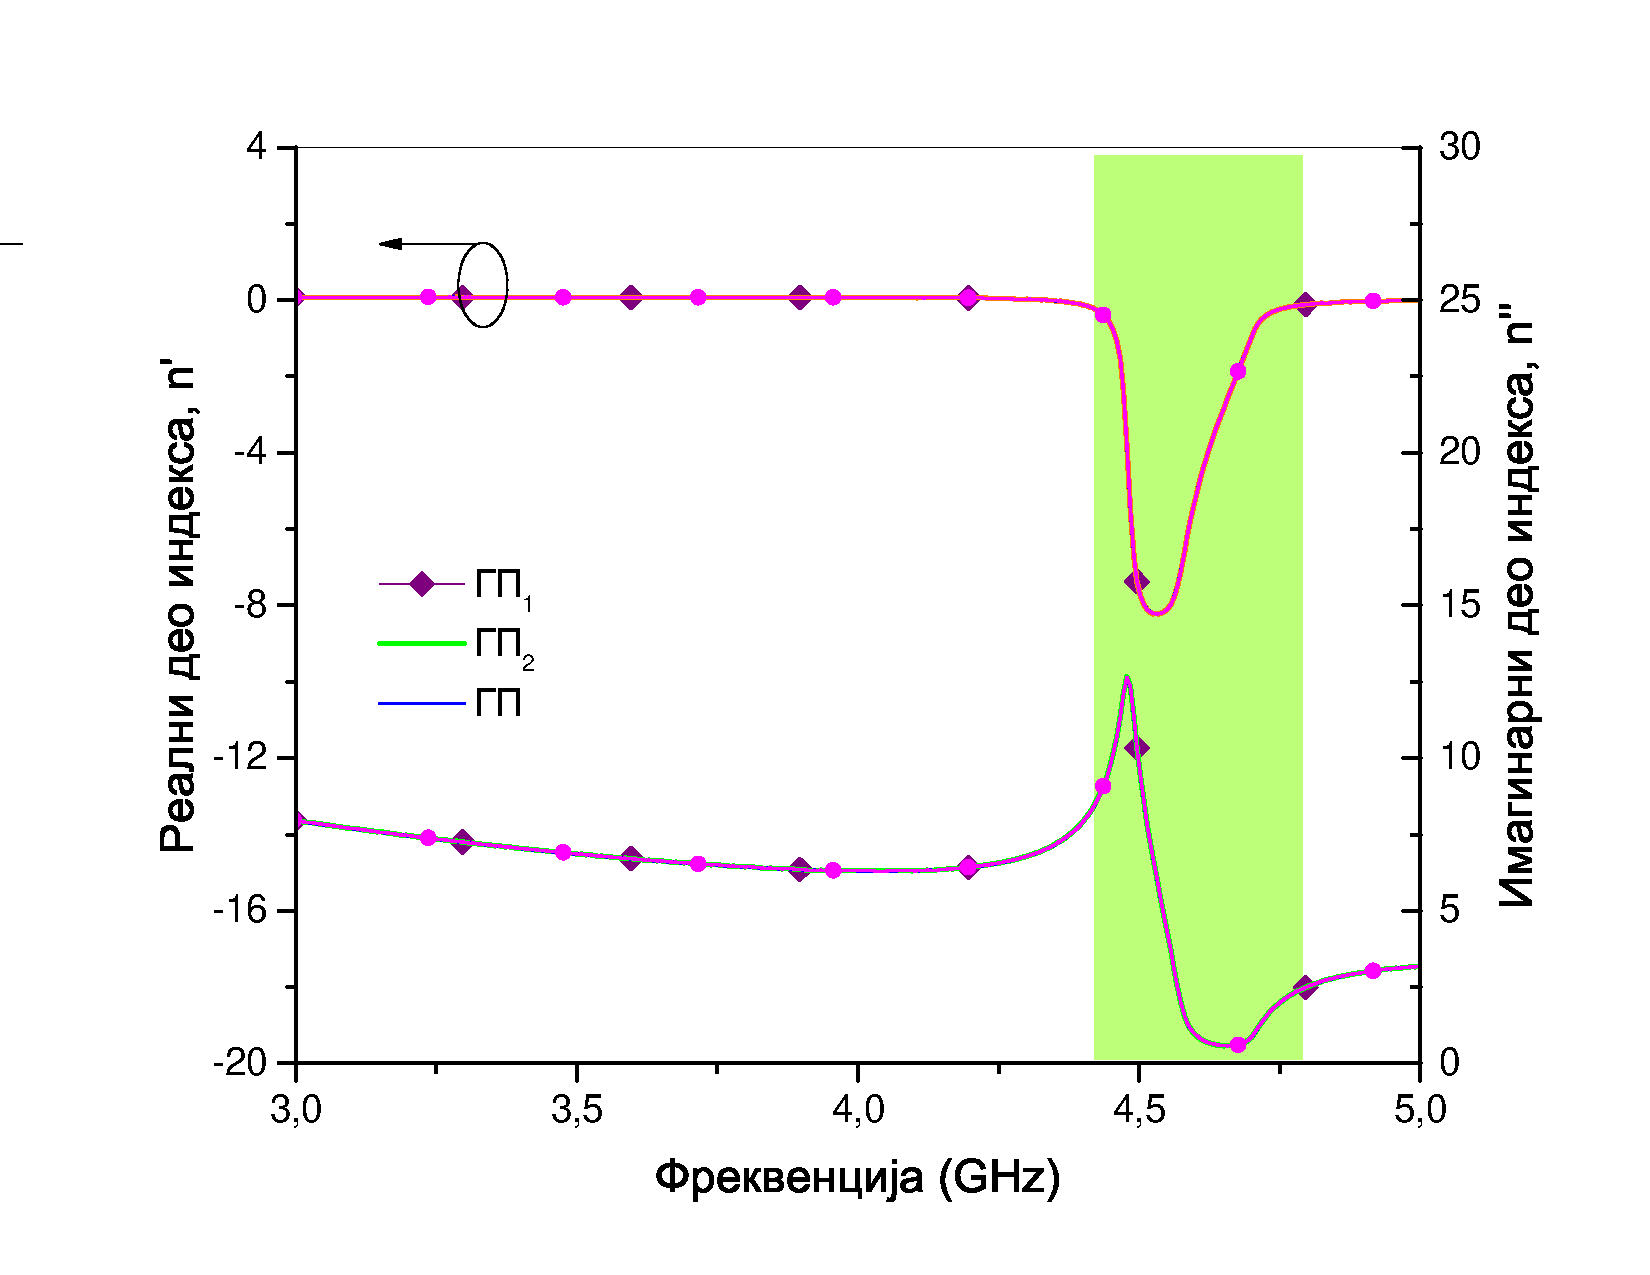
\includegraphics[width=0.6\textwidth]{slike/physcr/pod0/n}}
%\label{fig}}
\hfill
\subfloat[]{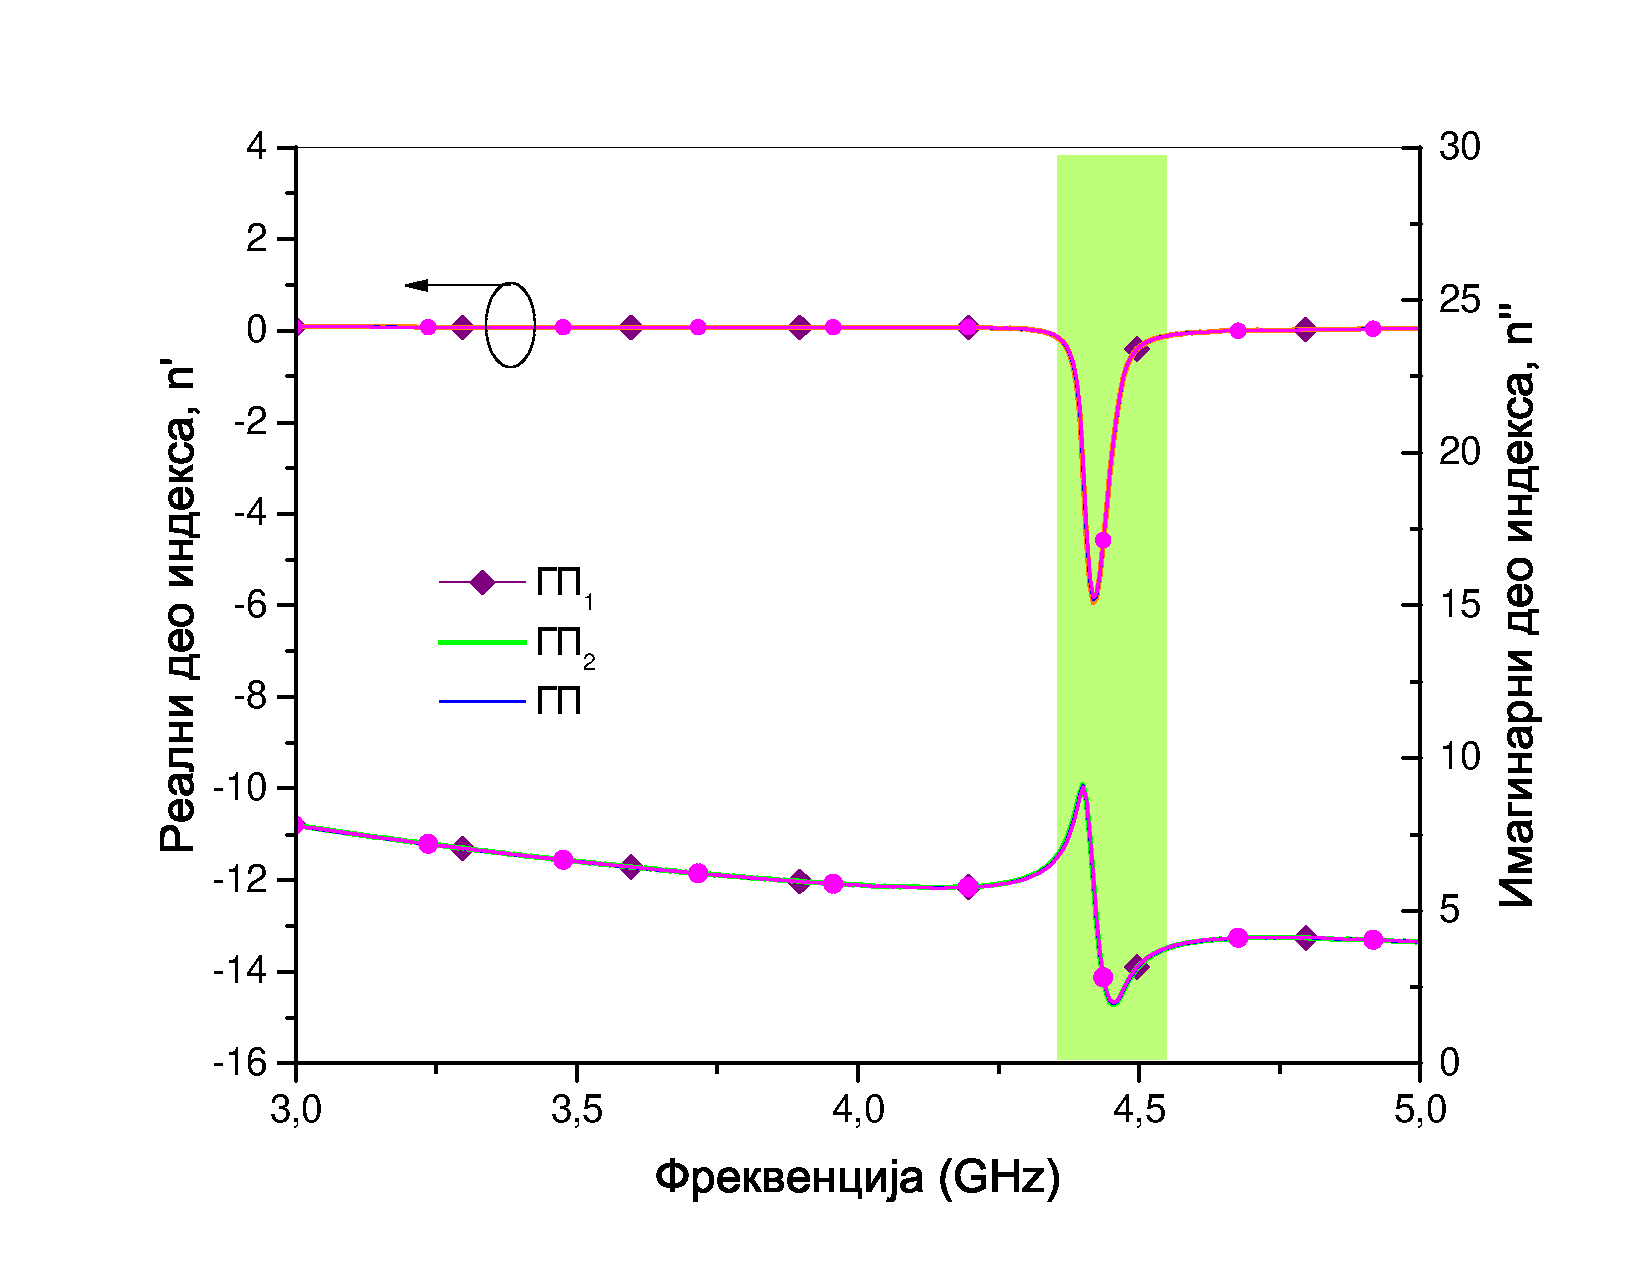
\includegraphics[width=0.6\textwidth]{slike/physcr/pod90/n}}
%\label{fig}}
\caption{Екстраховани индекс преламања: \labelaslike Осенчени делови означавају зоне са двоструко-негативним параметрима.}
\label{ph:fig4}
\end{figure} 

\begin{figure}[!t]
\centering
\subfloat[]{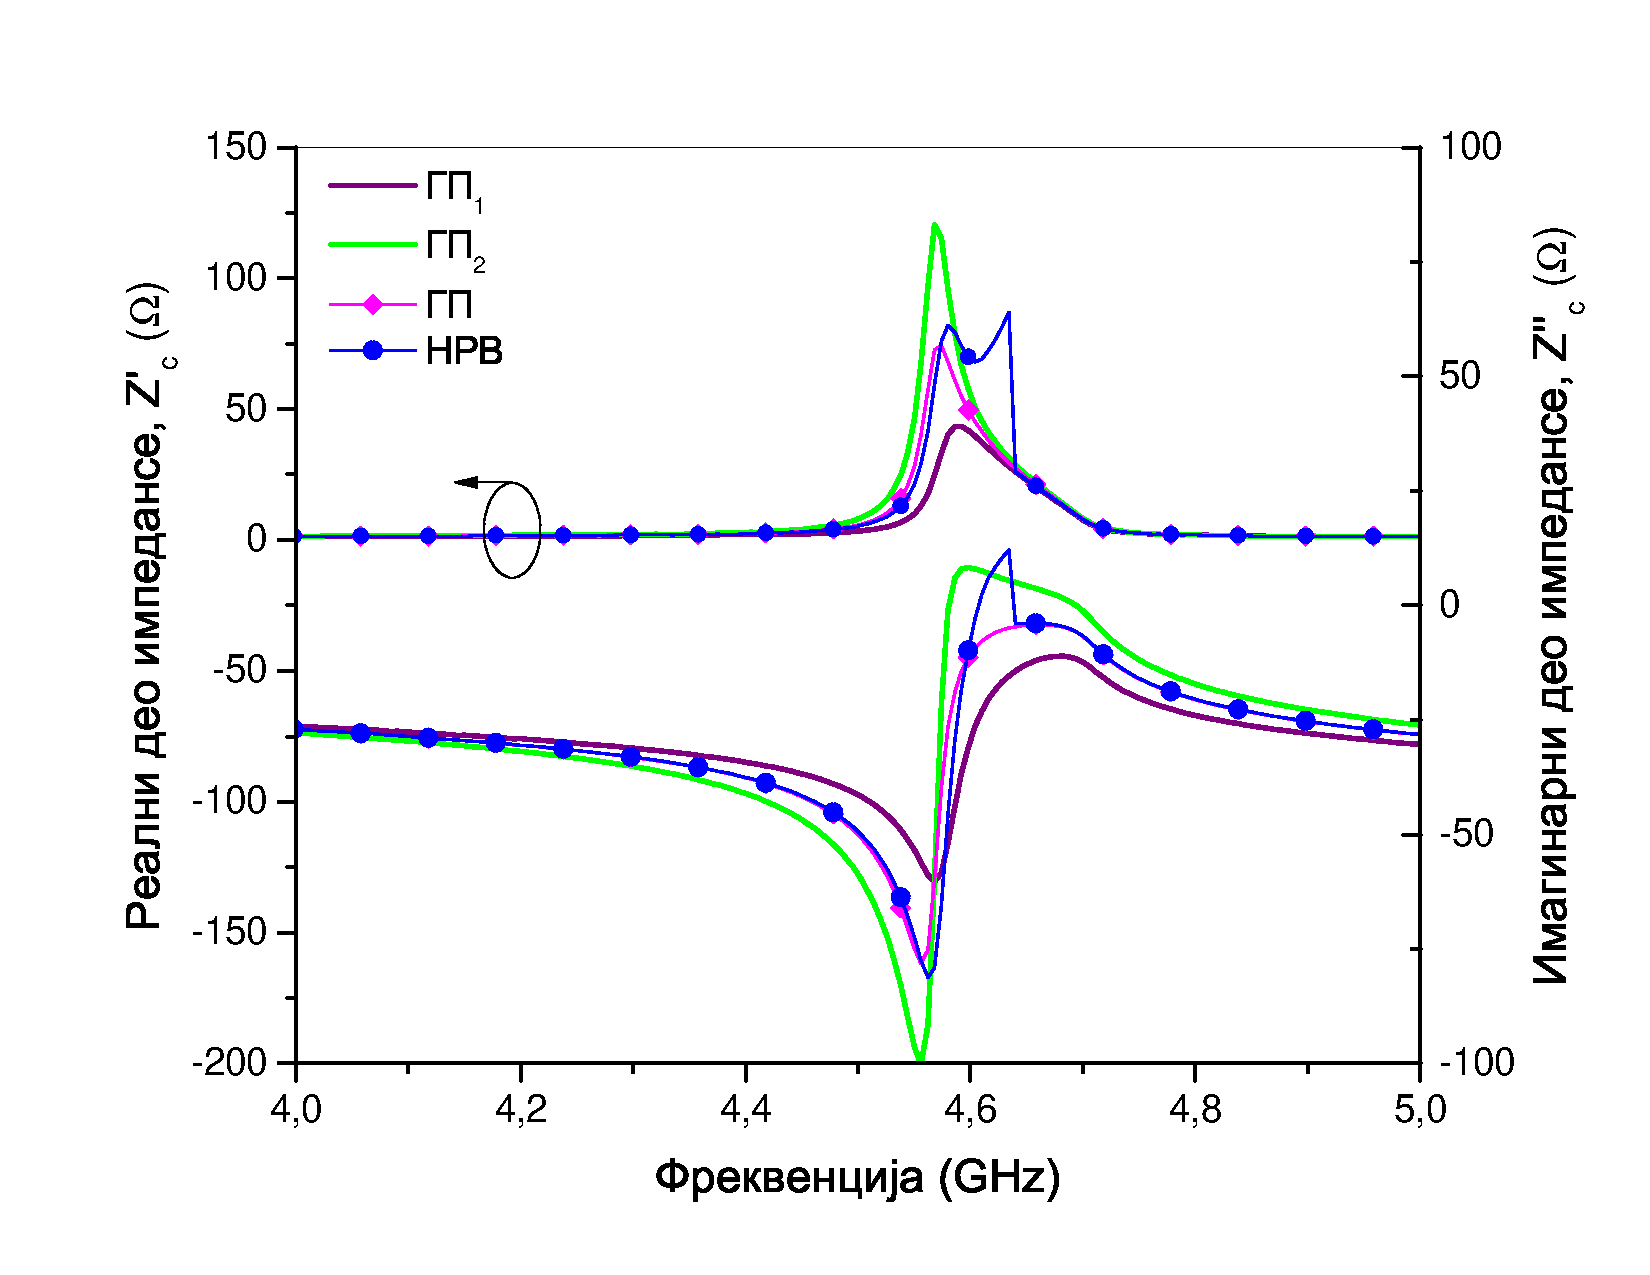
\includegraphics[width=0.6\textwidth]{slike/physcr/pod0/zc}}
%\label{fig}}
\hfill
\subfloat[]{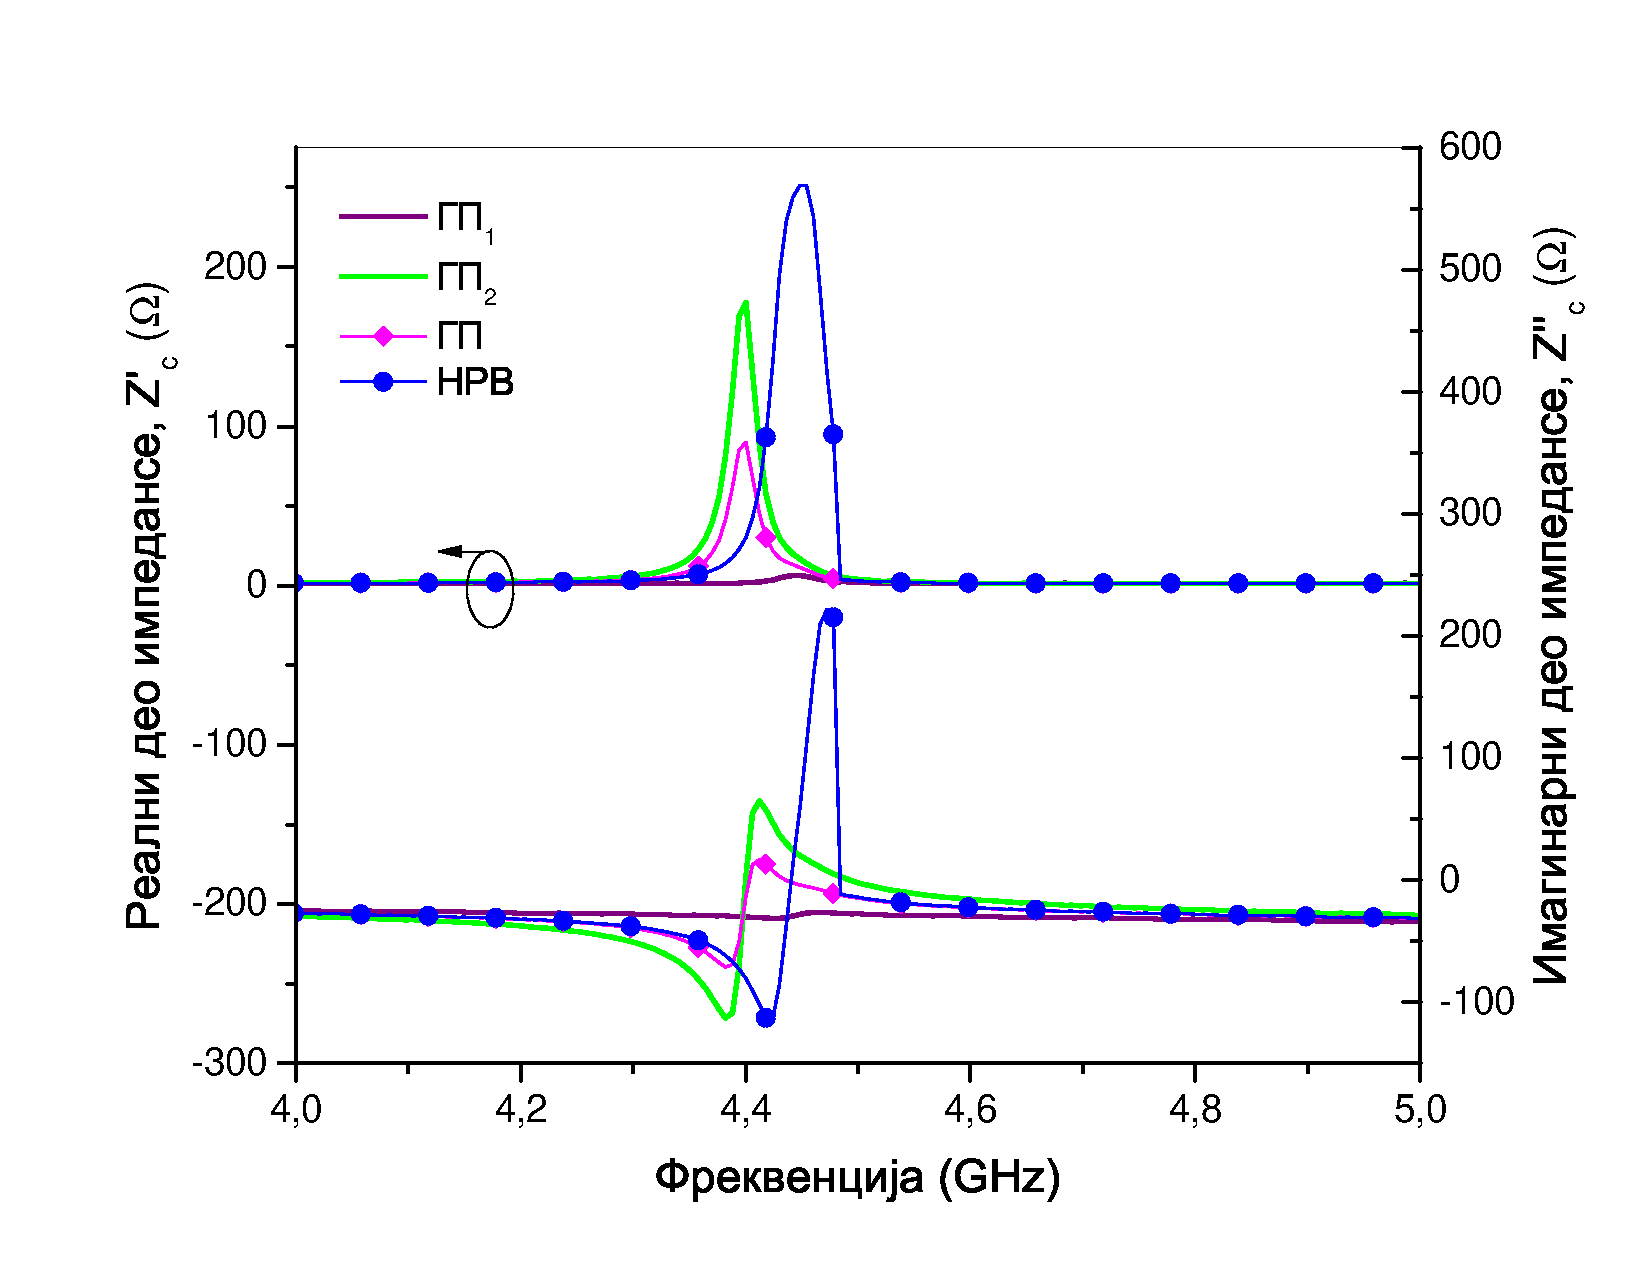
\includegraphics[width=0.6\textwidth]{slike/physcr/pod90/zc}}
%\label{fig}}
\caption{Екстрахована карактеристична импеданса: \labelaslike}
\label{ph:fig5}
\end{figure} 

\begin{figure}[!t]
\centering
\subfloat[]{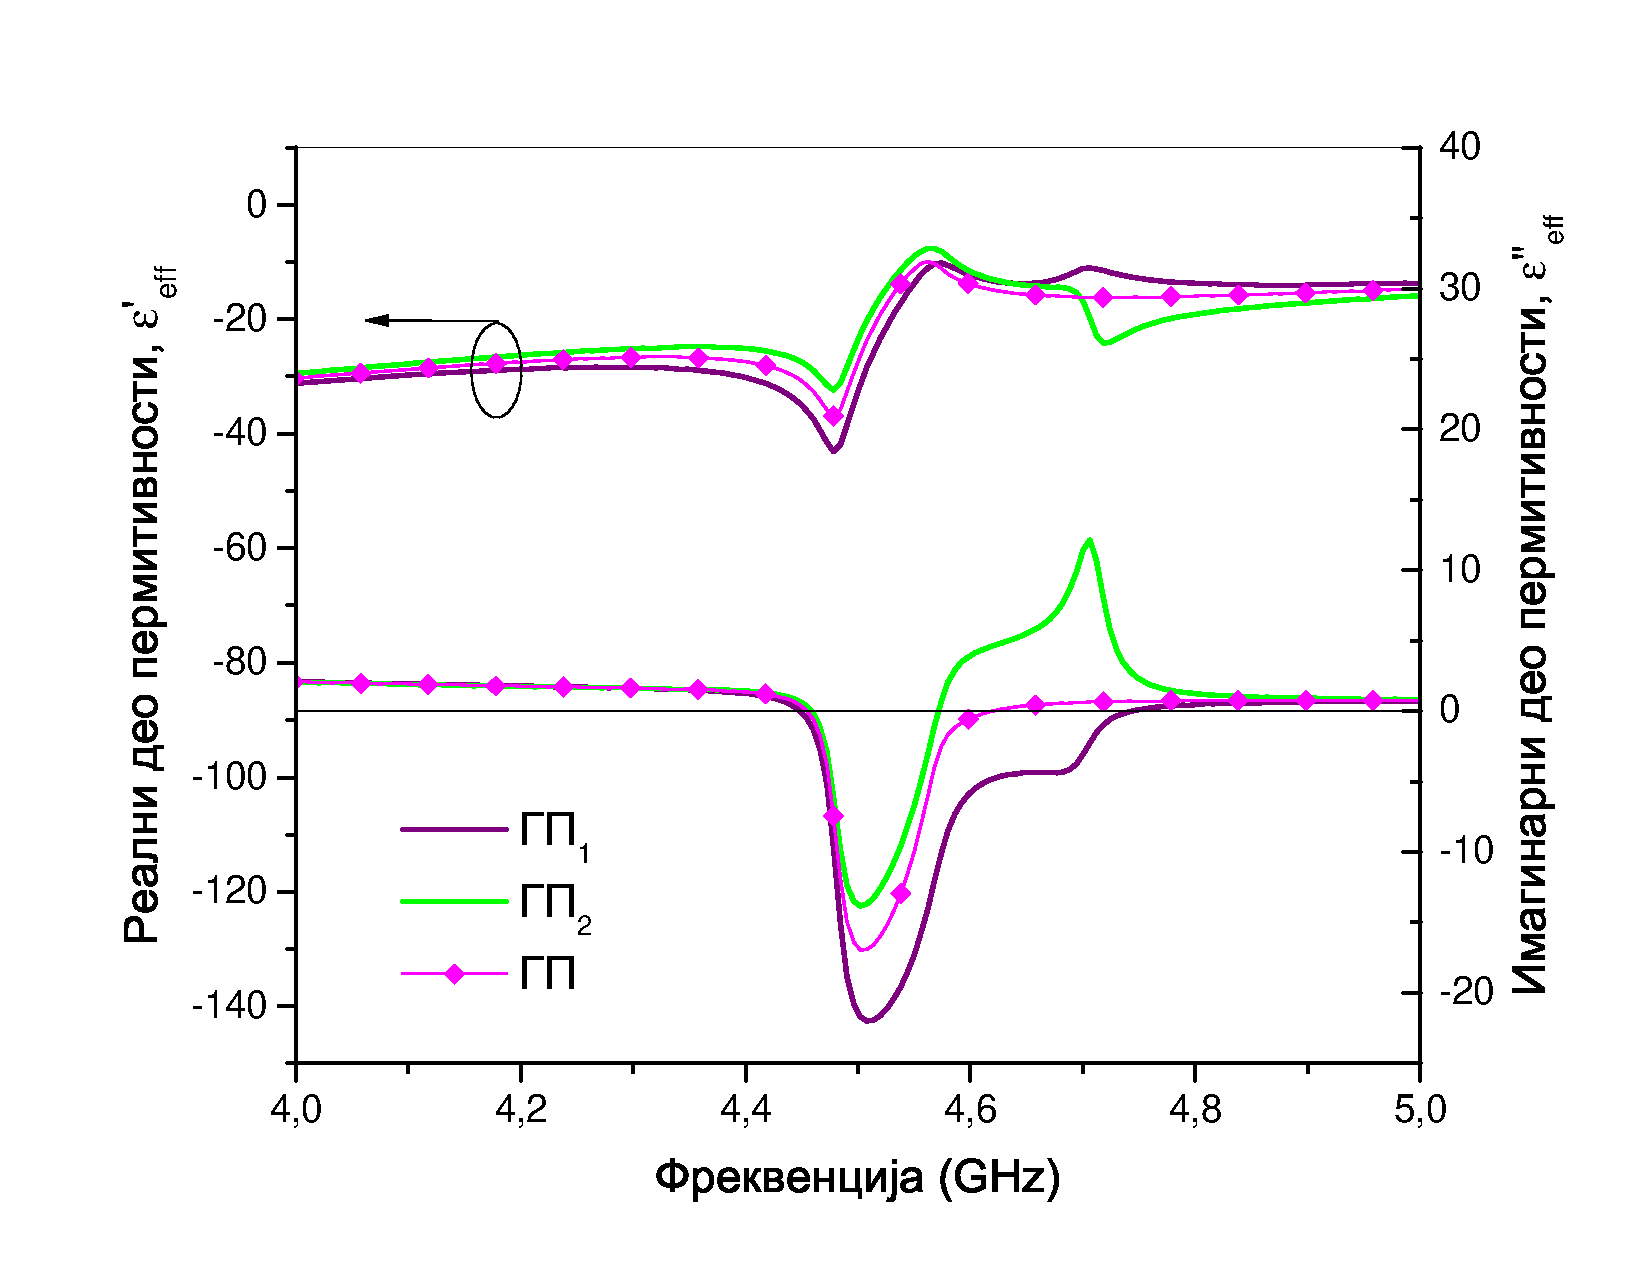
\includegraphics[width=0.6\textwidth]{slike/physcr/pod0/eps}
\label{ph:fig6a}}
\hfill
\subfloat[]{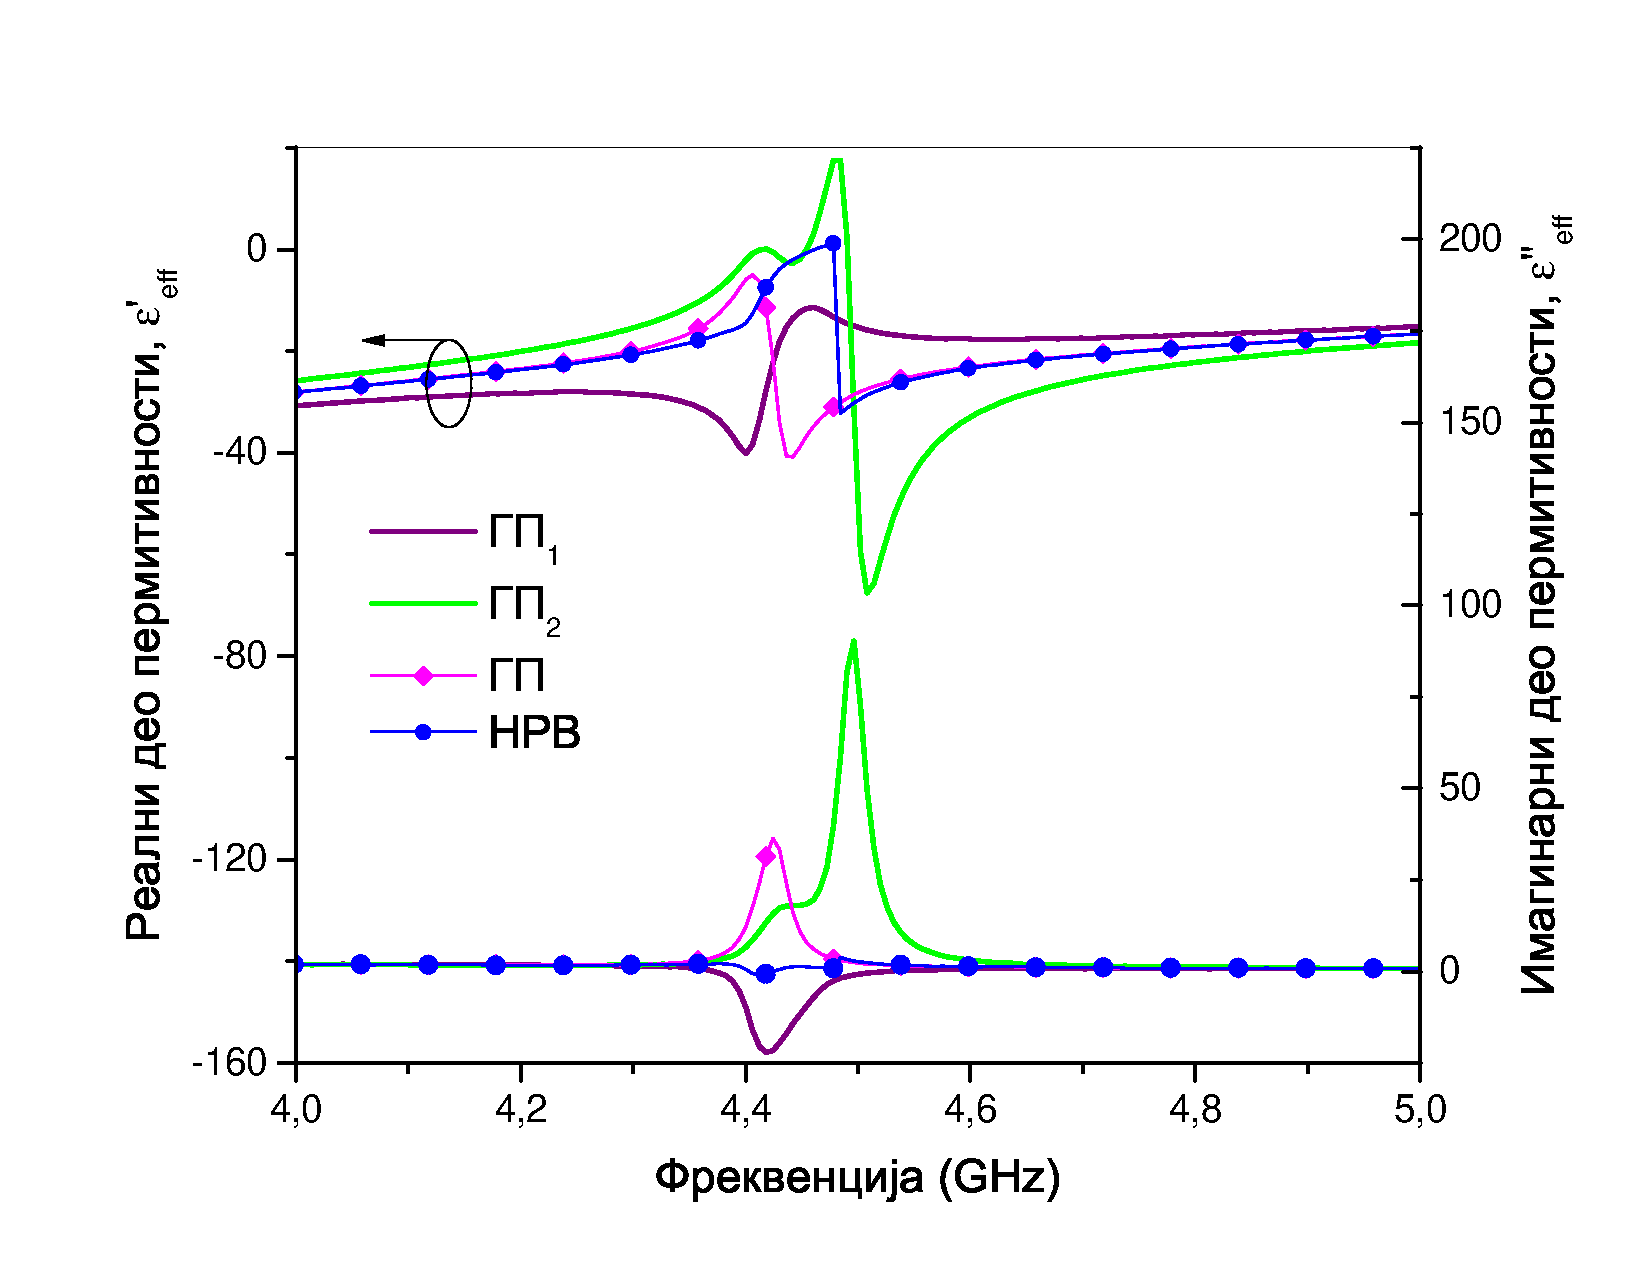
\includegraphics[width=0.6\textwidth]{slike/physcr/pod90/eps}
\label{ph:fig6b}}
\caption{Екстрахована ефективна пермитивност: \labelaslike}
\label{ph:fig6}
\end{figure} 

\begin{figure}[!t]
\centering
\subfloat[]{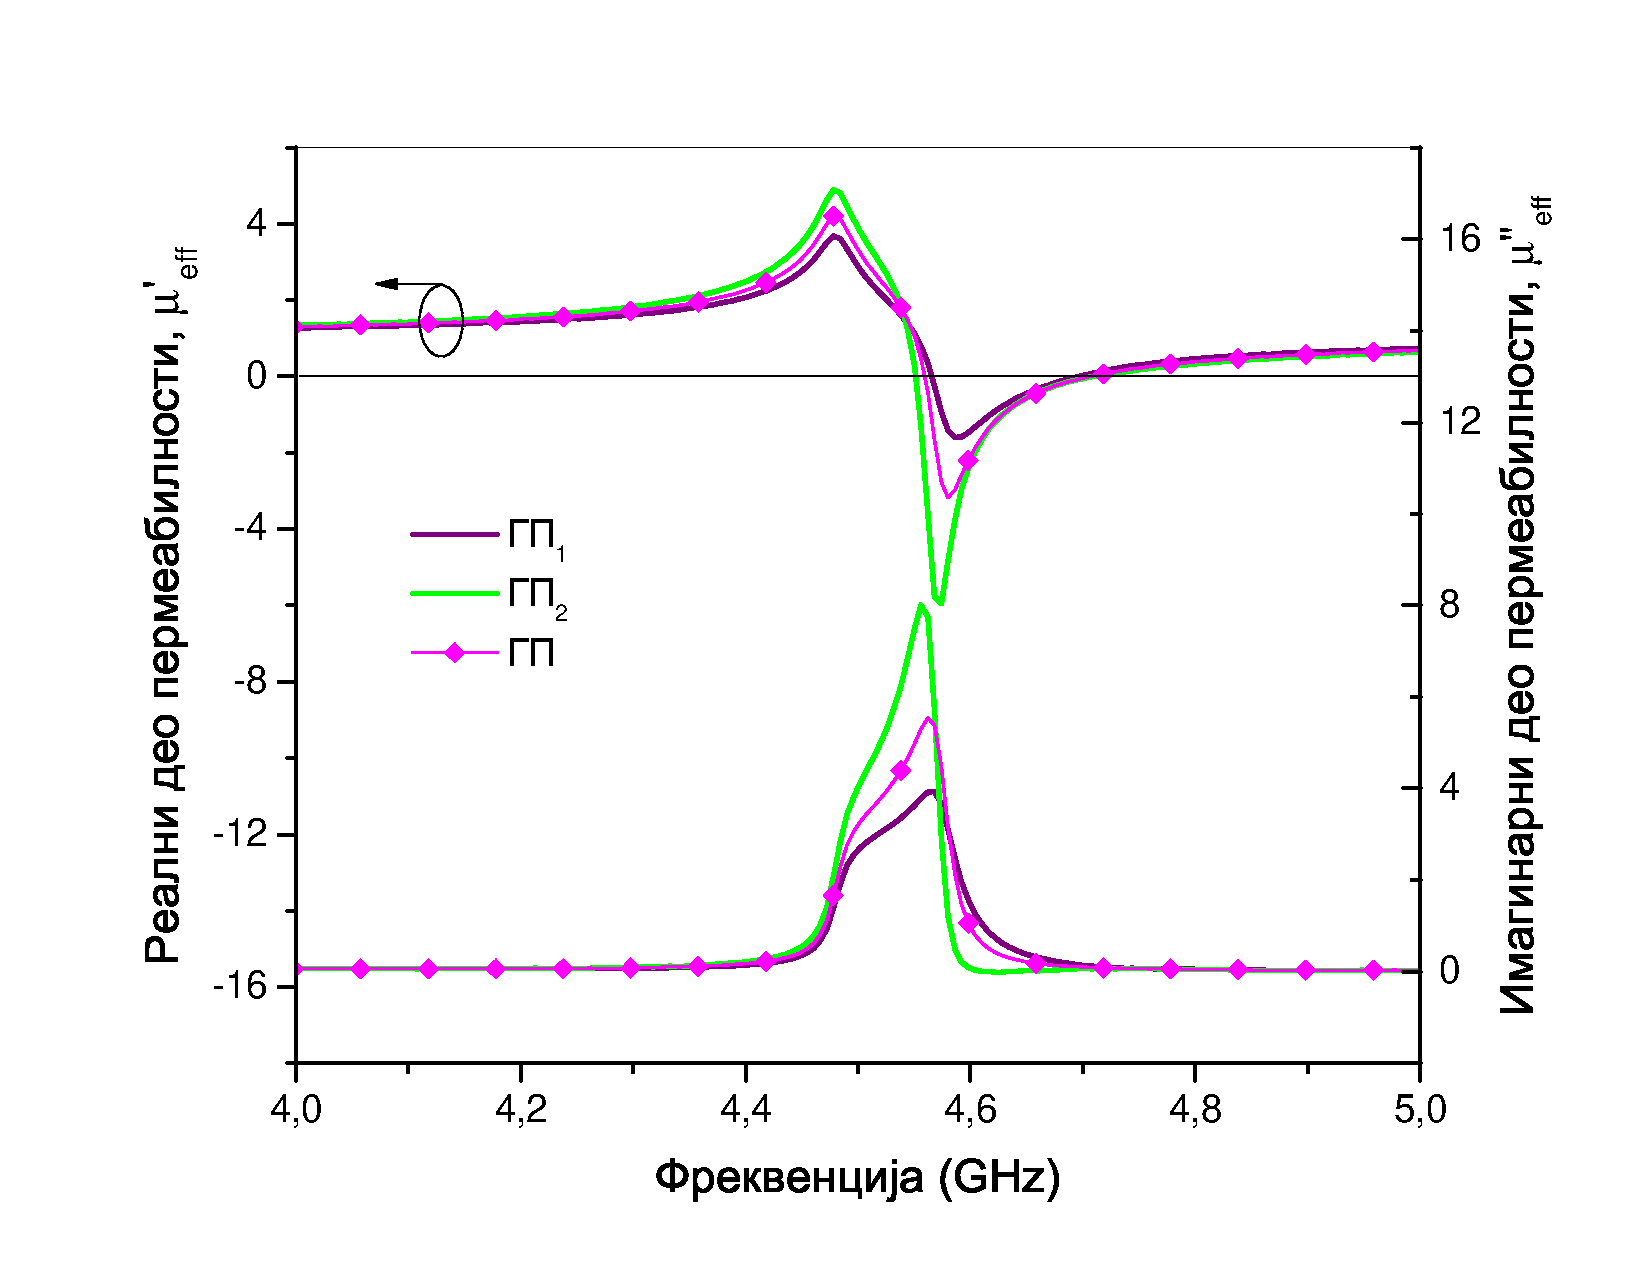
\includegraphics[width=0.6\textwidth]{slike/physcr/pod0/mi}
\label{ph:fig7a}}
\hfill
\subfloat[]{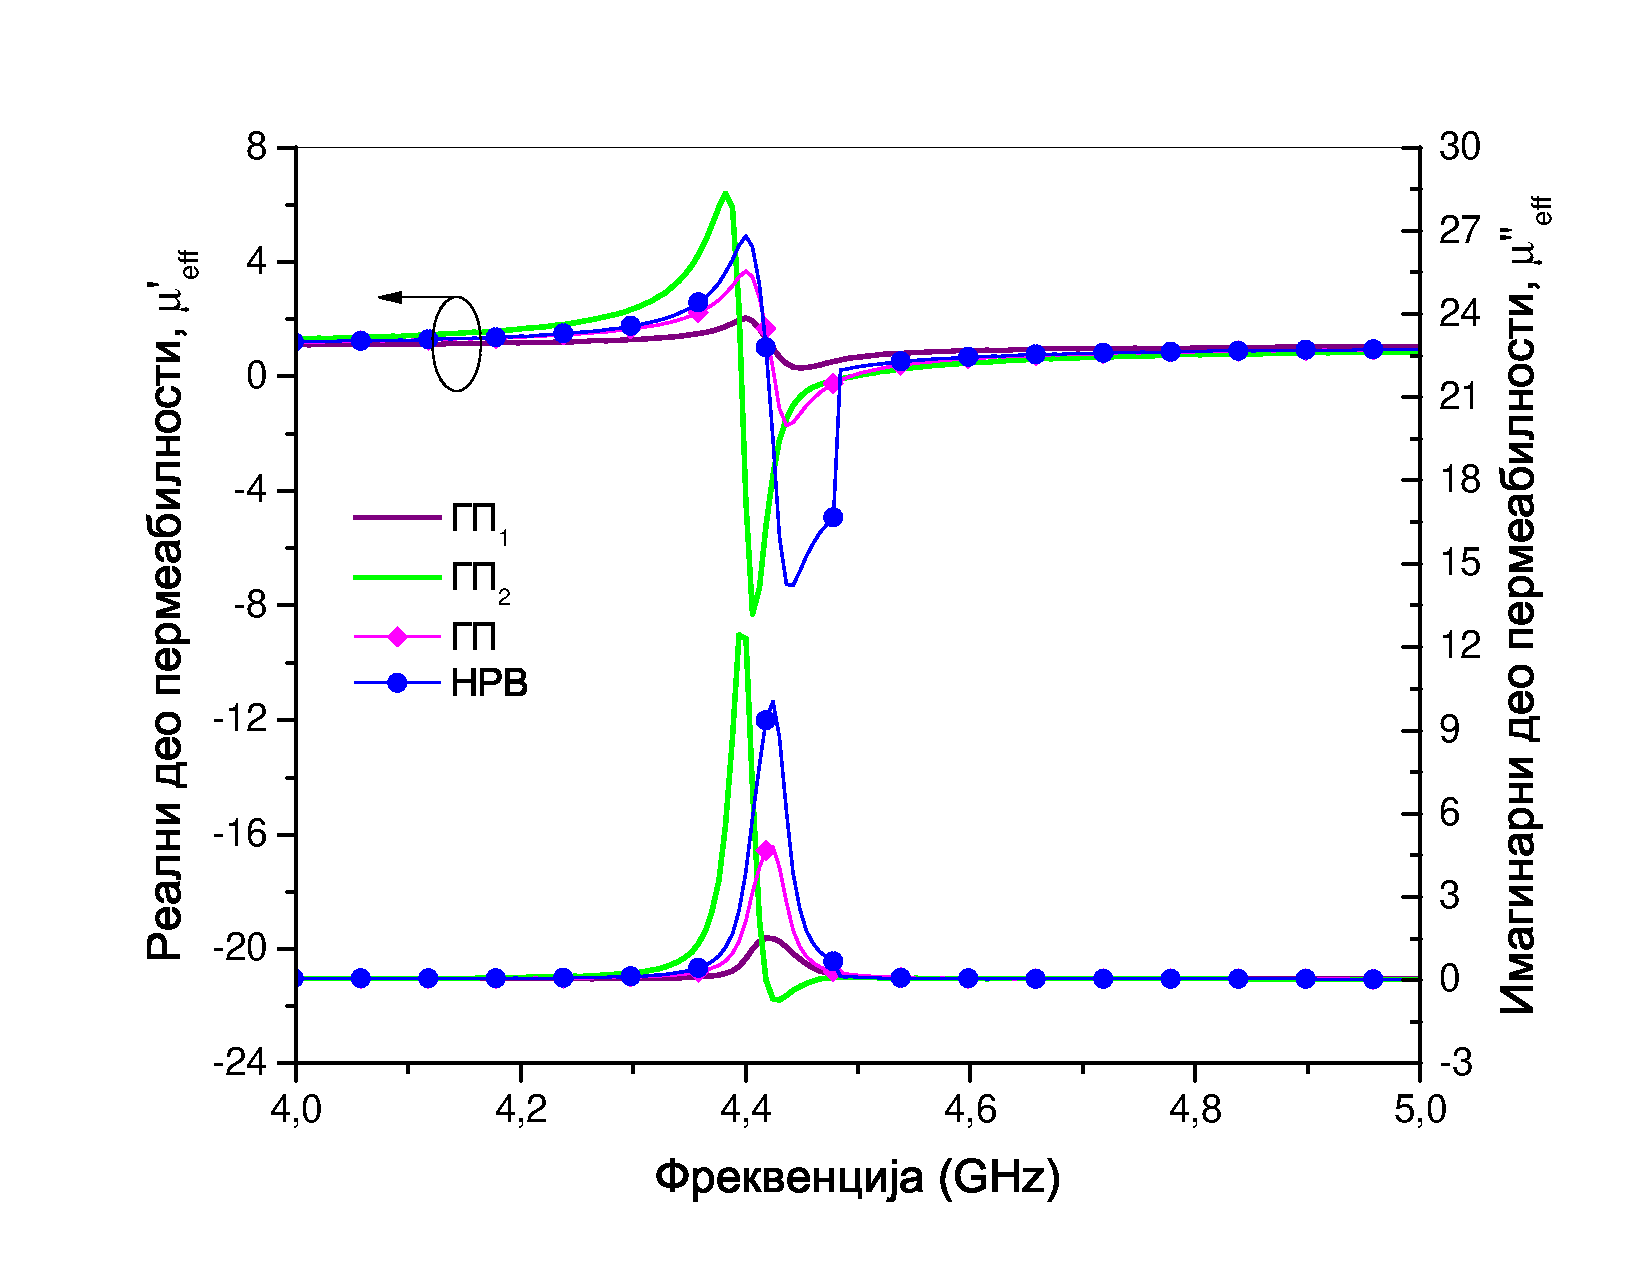
\includegraphics[width=0.6\textwidth]{slike/physcr/pod90/mi}
\label{ph:fig7b}}
\caption{Екстрахована ефективна пермеабилност: \labelaslike}
\label{ph:fig7}
\end{figure} 

\section{Валидација метода екстракције}\label{sekc4}
\subsection{Метод декомпозиције}
За проверу валидности предложене методе, може се користити независна симулација микрострип вода уроњеног у хомогени диелектрик са параметрима који одговарају екстрахованим вредностима, као што је приказано на сл.~\ref{slab}. Улазни микрострип водови су уроњени у ефективни диелектрик пермитивности $\varepsilon^{ML}_{eff}=\num{3.15}$. Приликом рачунања $Ѕ$-параметара, улазни водови се деембедују (\foreign{de-embedding}). Описана процедура се може непосредно применити за реконструкцију $Ѕ$-параметара добијених НРВ екстракцијом, која користи изотропни медијум описан са $\varepsilon$ и $\mu$, међутим [у тренутку писања рада] ауторима није било познато постојање програма за ЕМ анализу способног за рад са бианизотропним медијима.
\begin{figure}[!t]
\centering
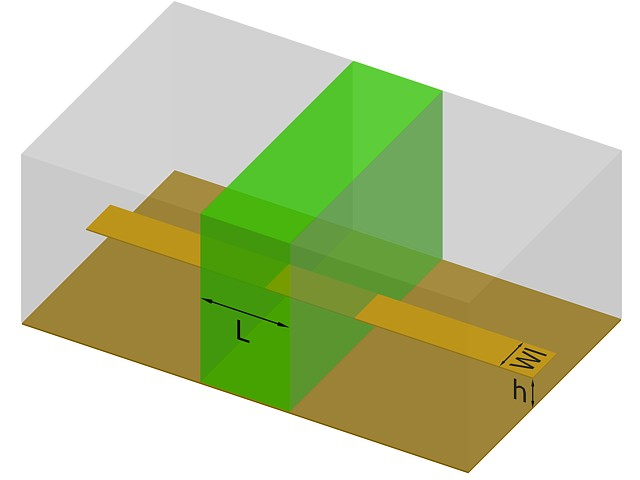
\includegraphics[width=0.6\columnwidth]{slike/slab.jpeg}
\caption{Слој ефективног медијума, који одговара асиметричној јединичној ћелији (зелени квадар) и улазни микрострип водови уроњени у ефективни диелектрик (светлосиви [квадри]). Релевантне димензије: $L=L_r+2L_m$, $h=h_1+h_2$, где су $L_r$, $L_m$, $h_1$, $h_2$ и $W_l$ дати на сл.~\ref{fig4}.}
\label{slab}
\end{figure}

Због тога, предложено је следеће [заобилазно] решење: симулирање два изотропна слоја, чији параметри одговарају онима добијеним $ГП_1$ и $ГП_2$ екстракцијама, на основу чега се добијају два сета $ABCD$ параметара, означених као $ABCD_{ГП1}$ and $ABCD_{ГП2}$, респективно. Сада, ако се пажљивије размотри релација (\ref{decomp}), примећује се да она представља дијагонализацију матрице, при чему $e^{\pm \gamma l}$ представљају сопствене вредности, а колоне матрице $Q$ сопствене векторе. Из (\ref{slicnost}) и (\ref{decomp}) следи да ће се матрице $ABCD_{ГП1,2}$, пошто оне подразумевају само једну вредност импедансе $Z_{c1,2}$, дијагонализовати у следећем облику:
\begin{equation}\label{decomp2}
ABCD_{ГП1,2} = Q_{1,2}\: \mathrm{diag}(e^{\gamma l},e^{-\gamma l})\: Q_{1,2}^{-1};
\end{equation}
where
\begin{equation}
Q_{1,2} = 
\begin{bmatrix}
1 & 1 \\
\frac{1}{Z_{c1,2}} & -\frac{1}{Z_{c1,2}}
\end{bmatrix}.
\end{equation}
Приметимо да су сопствене вредности $e^{\pm \gamma l}$ једнаке за све три матрице.

Из симулације слојева $ГП_{1,2}$ добијају се два сета $S$-параметара, који се могу конвертовати у $ABCD_{ГП1,2}$. Затим се врши дијагонализација ових матрица да би се добио облик (\ref{decomp2}). Оваква дијагонализација је лако доступна у програмским пакетима попут МАТЛАБ-а, и неопходно је само распоредити сопствене вредности и векторе на исти начин као у (\ref{decomp2}), што се може урадити на основу критеријума пасивности (\ref{pasivnost}). Сада је могуће добити матрицу $Q$ као
\begin{equation}
Q =
\begin{bmatrix}
Q_1(1,1) & Q_2(1,2) \\
Q_1(2,1) & Q_2(2,2)
\end{bmatrix},
\end{equation}
и, коначно, тражену $ABCD$ матрицу у складу са релацијом (\ref{decomp}).

\subsection{Јединичне ћелије са паралелним процепима}

$S$-параметри добијени описаним поступком, за јединичну ћелију са процепима паралелним и даље од вода (видети сл.~\ref{fig4b}), упоређени са оригиналним симулацијама, приказани су на сл.~\ref{val_pod180_mag}-\ref{val_pod180_ang}, за ГП и НРВ екстракције. НРВ метод (сл.~\ref{val_pod180nrw_mag} и \ref{val_pod180nrw_ang}) резултира са симетричним одзивом (због чега је само један коефицијент рефлексије, $S_{11}^{eff}=S_{22}^{eff}$, реконструисан), што очигледно не успева да тачно репродукује рефлексију у регионима са наглашеном асиметријом (осенченим на графику). Ово је највидљивије у фази, где се добијена вредност понања као средња вредност оригиналних фаза $S_{11}$ и $S_{22}$ (ово је очекивано због коришћене процедуре усредњавања).
\begin{figure}[!t]
\centering
\subfloat[]{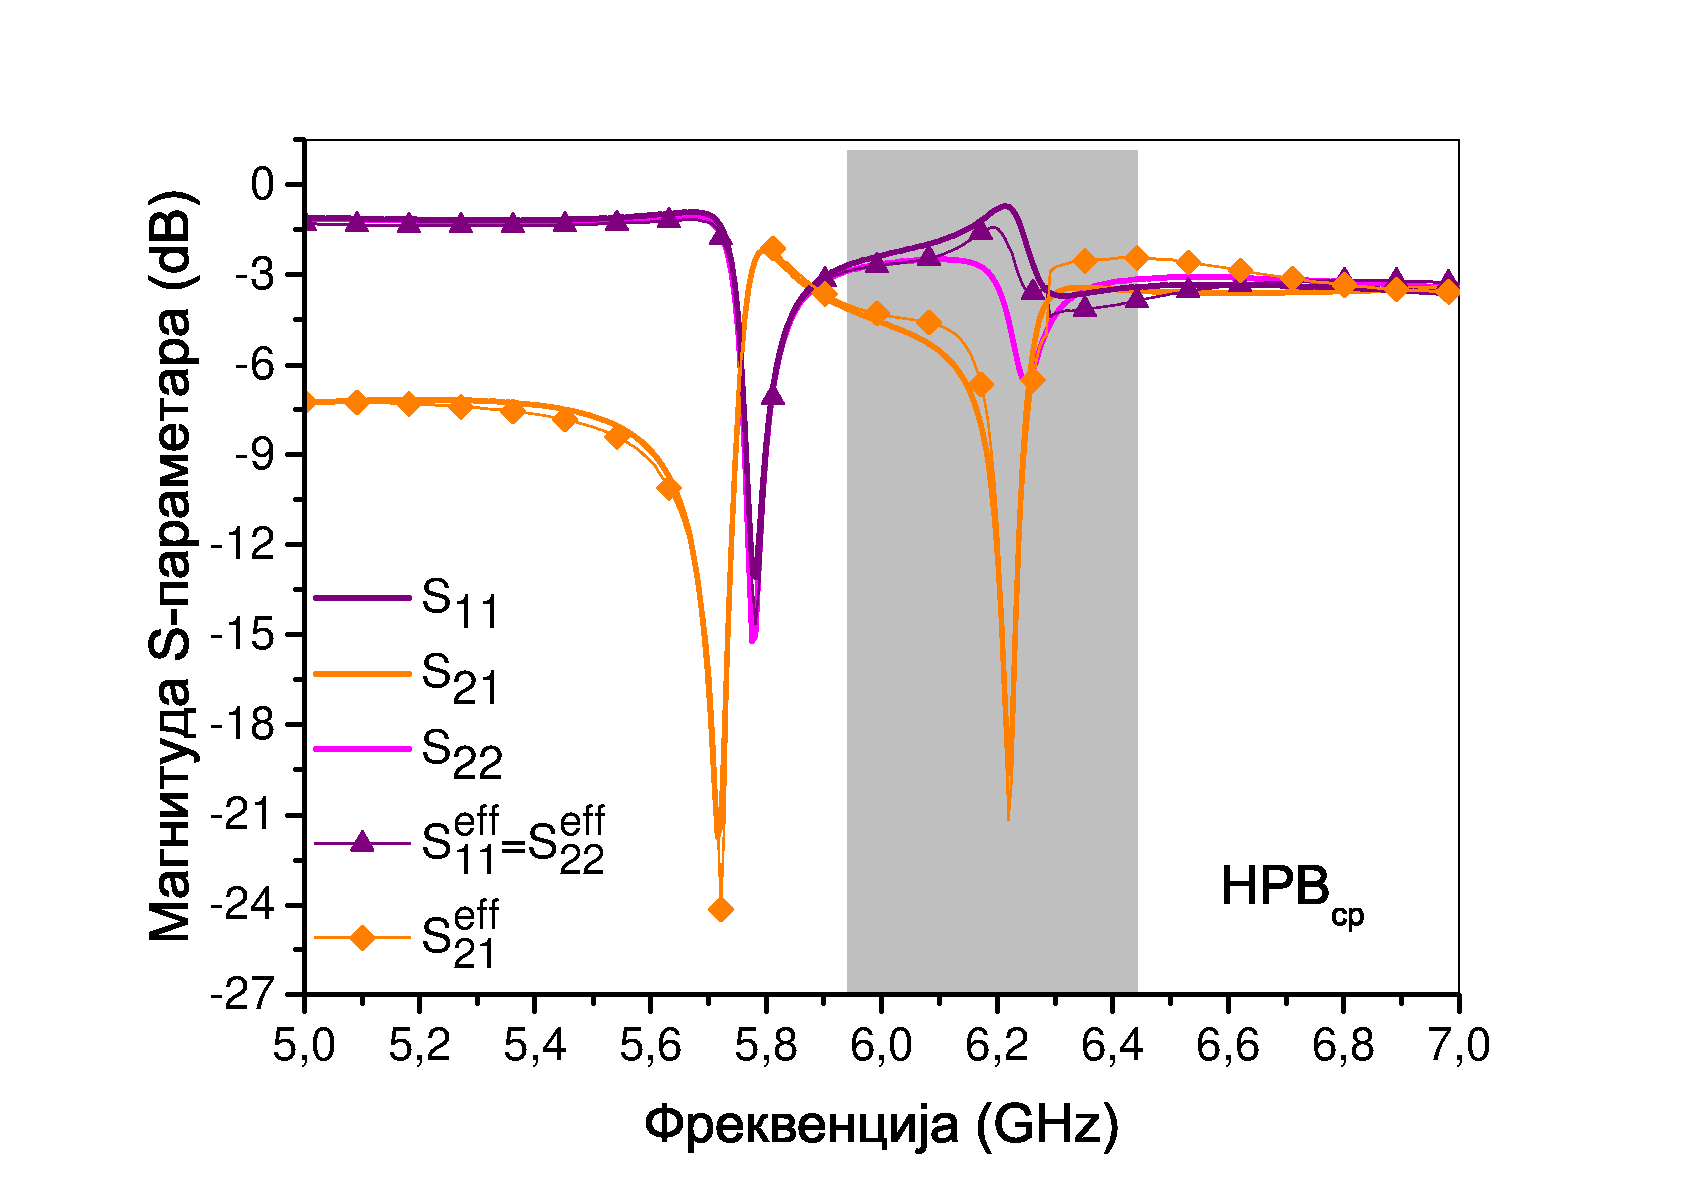
\includegraphics[scale=\SkalaC]{slike/val180nrw_mag.pdf}
\label{val_pod180nrw_mag}}
\subfloat[]{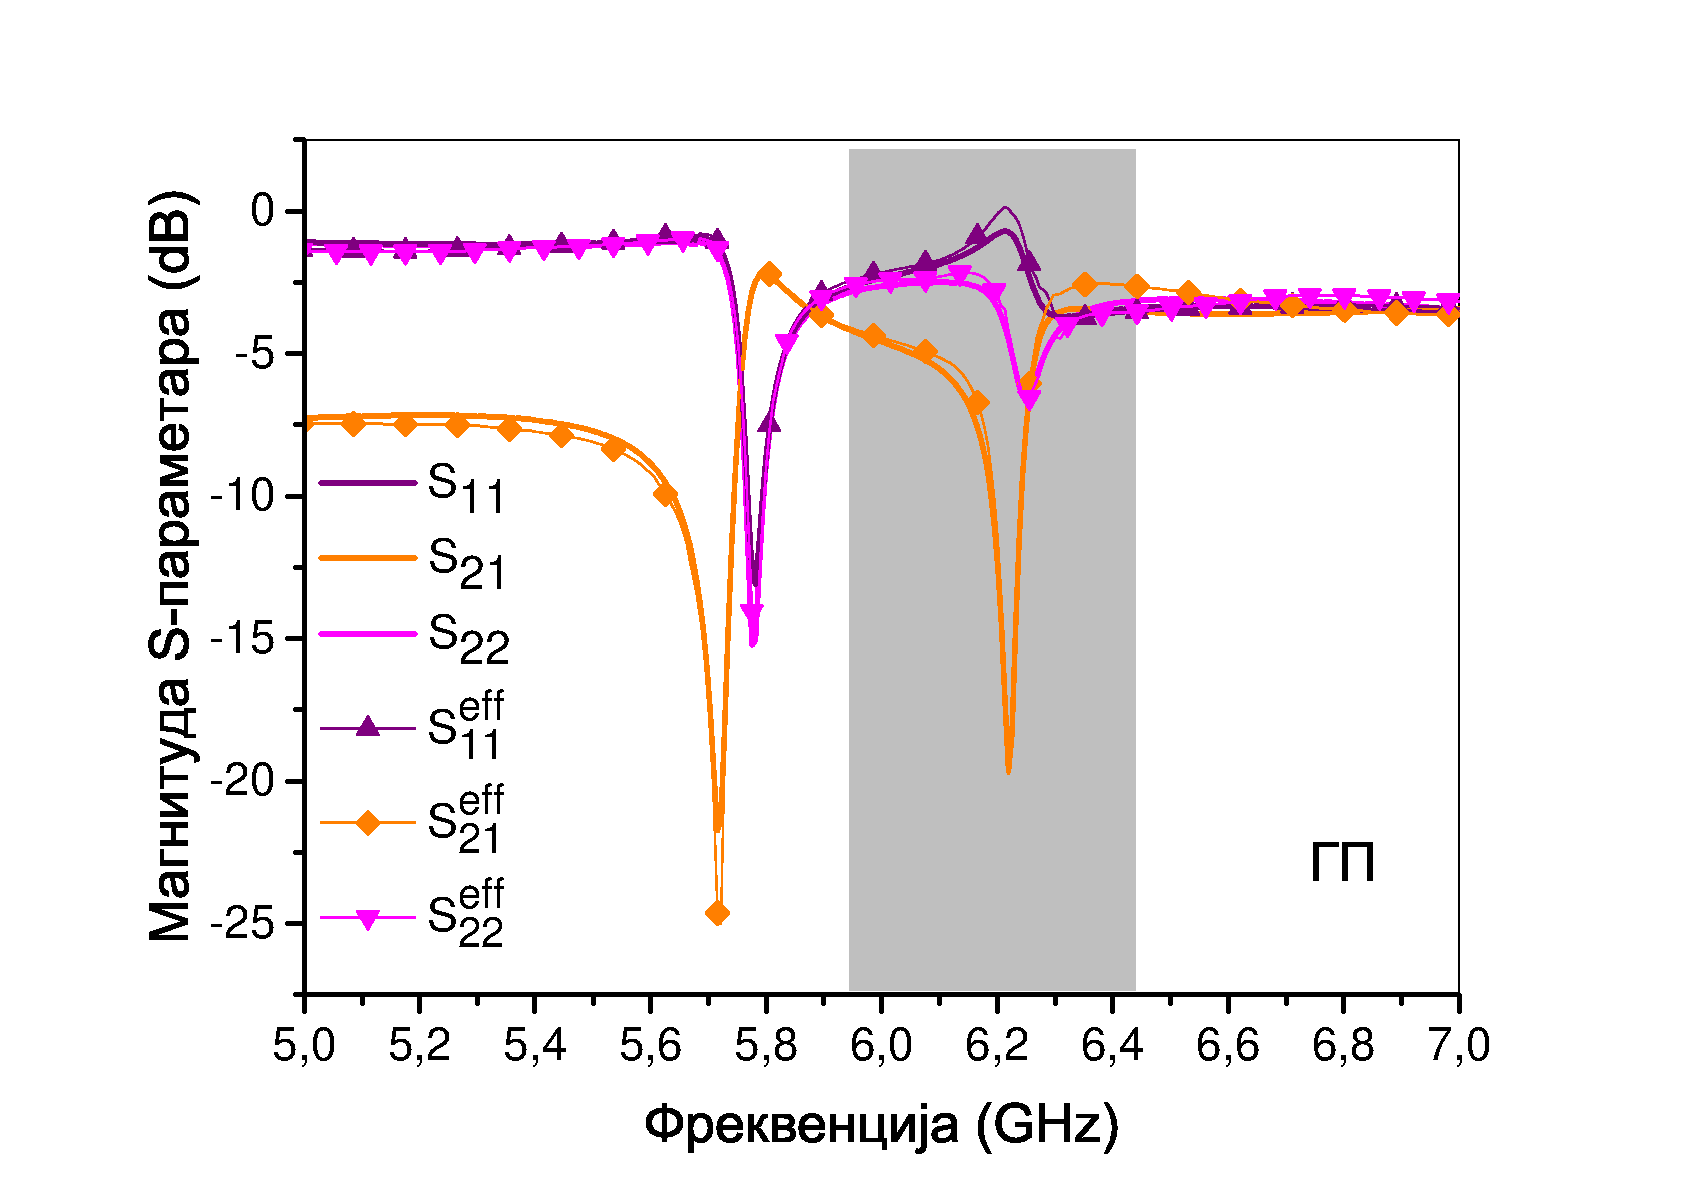
\includegraphics[scale=\SkalaC]{slike/val180ga_mag.pdf}
\label{val_pod180ga_mag}}
\caption{Магнитуда $S$-параметара симулираних и реконструисаних коришћењем ефективних параметара: (а) $НРВ_{СР}$ и (б) ГП екстракције. Осенчени делови означавају опсеге у којима се магнитуда $S_{11}$ и $S_{22}$ разликује.}
\label{val_pod180_mag}
\end{figure}
\begin{figure}[!t]
\centering
\subfloat[]{\includegraphics[scale=\SkalaC]{slike/val180nrw_ang.pdf}
\label{val_pod180nrw_ang}}
\subfloat[]{\includegraphics[scale=\SkalaC]{slike/val180ga_ang.pdf}
\label{val_pod180ga_ang}}
\caption{Фаза $S$-параметара симулираних и реконструисаних коришћењем ефективних параметара: (а) $НРВ_{СР}$ и (б) ГП екстракције.}
\label{val_pod180_ang}
\end{figure}

ГП метод, међутим, јасно разликује различите вредности коефицијената рефлексије, које су врло близу оригиналних вредности (видети сл.~\ref{val_pod180ga_mag} и \ref{val_pod180ga_ang}). Јасно се види да ефективни параметри добијени ГП методом омогућавају реконструкцију свих $S$-параметара, што није случај за $НРВ_{СР}$ методу, која омогућава реконструкцију само $S_{21}$, али не и $S_{11}$ и $S_{22}$ у опсезима где је присутна асиметрија. Ван тих опсега, ћелија има симетричан одзив и обе методе раде коректно.

\subsection{Јединичне ћелије са нормалним процепима}
Резултати за јединичну ћелију са нормалним процепом, са горњим процепом ближе воду (видети сл.~\ref{norm1}), упоређени са оригиналним симулацијама, су приказани на сл.~\ref{val_pod90_mag}-\ref{val_pod90_ang}, за $НРВ_{СР}$ и ГП екстракције. Поново, $НРВ_{СР}$ метод (видети сл.~\ref{val_pod90nrw_mag} и \ref{val_pod90nrw_ang}) репродукује само средњу вредност рефлексије, при чему је неслагање у овом случају још уочљивије, услед веће асиметричност ћелије. ГП метод поново блиско репродукује оба коефицијента рефлексије (видети сл.~\ref{val_pod90ga_mag} и \ref{val_pod90ga_ang}). Оба метода испољавају одређена неслагања, посебно у магнитуди $S_{21}$ изнад друге резонансе, која се могу приписати апроксимацији оригиналног вода, на коме се простире квази-ТЕМ мод, са водом у ефективном диелектрику, на коме се простире прави ТЕМ мод.
\begin{figure}[!t]
\centering
\subfloat[]{\includegraphics[scale=\SkalaC]{slike/val90nrw_mag.pdf}
\label{val_pod90nrw_mag}}
\subfloat[]{\includegraphics[scale=\SkalaC]{slike/val90ga_mag.pdf}
\label{val_pod90ga_mag}}
\caption{Магнитуда $S$-параметара симулираних и реконструисаних коришћењем ефективних параметара: (а) $НРВ_{СР}$ и (б) ГП екстракције. Осенчени делови означавају опсеге у којима се магнитуда $S_{11}$ и $S_{22}$ разликује.}
\label{val_pod90_mag}
\end{figure}
\begin{figure}[!t]
\centering
\subfloat[]{\includegraphics[scale=\SkalaC]{slike/val90nrw_ang.pdf}
\label{val_pod90nrw_ang}}
\subfloat[]{\includegraphics[scale=\SkalaC]{slike/val90ga_ang.pdf}
\label{val_pod90ga_ang}}
\caption{Фаза $S$-параметара симулираних и реконструисаних коришћењем ефективних параметара: (а) $НРВ_{СР}$ и (б) ГП екстракције.}
\label{val_pod90_ang}
\end{figure}

%\subsection{Ивично спрегнути \emph{физскрипта}}
%\begin{figure}[!t]
%\centering
%\subfloat[]{\includegraphics[scale=\SkalaA]{slike/physcr/pod0/valmag}}
%%\hspace*{1cm}
%\subfloat[]{\includegraphics[scale=\SkalaA]{slike/physcr/pod90/valmag}}
%\caption{Magnitudes of $S$-parameters simulated and recovered using the effective bianisotropic parameters: \labelaslike}
%\label{ph:fig8}
%\end{figure} 

%\begin{figure}[!t]
%\centering
%\subfloat[]{\includegraphics[scale=\SkalaA]{slike/physcr/pod0/valfaza}}
%%\hspace*{1cm}
%\subfloat[]{\includegraphics[scale=\SkalaA]{slike/physcr/pod90/valfaza}}
%\caption{Phases of $S$-parameters simulated and recovered using the effective bianisotropic parameters: \labelaslike}
%\label{ph:fig9}
%\end{figure} 

\section{Закључак}

У овом поглављу приказана је генералисана процедура за екстракцију ефективних параметара за метаматеријале на бази водова са асиметричном јединичном ћелијом. За описивање асиметрије, користи се еквивалентни бианизотропни медијум, који поред стандардних ефективних параметара поседује два додатна, $u$ и $\eta$, који су корисни као квантификација асиметричности. 

Изведен је нови услов за негативни индекс преламања у бианизотропној средини. У поређењу са критеријумом за изотропне средине, услов је релаксиран у опсезима где су реални и имагинарни део параметра $u$ истог знака, а пооштрен тамо где су различитог знака.

Предложена генералисана процедура и НРВ метод са усредњавањем примењени су на нове дуал-бенд јединичне ћелије. Оне се састоје од СРР-ова са процепима помереним у односу на центар одговарајуће ивице, постављеним један изнад другог.

Показано је да јединичне ћелије са паралелним процепима имају асиметрични одзив само око једне од резонанси, док су у остатку опсега симетричне. За разлику од тога, ћелије са нормалним процепима имају изражен асиметрични одзив око обе резонансе. Ефективна пермитивност и пермеабилност, добијене помоћу два метода, знатно се разликују, не само по апсолутним вредностима, већ некад имају и супротне знакове.

Показано је да НРВ процедура са усредњавањем даје тачан индекс преламања, али погрешне ефективне вредности пермитивности, пермеабилности и карактеристичне импедансе, и да се може користити само када је асиметрија веома слаба. Ово је потврђено поступком валидације, у коме је симулиран слој ефективног медијума са одговарајућим параметрима. Применом ГП метода, могуће је реконструисати вредности свих $Ѕ$-параметара, што није случај за параметре добијене НРВ поступком.


\newcommand{\SkalaA}{0.1}
\newcommand{\SkalaB}{0.5}
\newcommand{\SirA}{2.0cm}
%\newcommand{\SirB}{5.8cm}
\newcommand{\SirB}{0.8\textwidth}

\newcommand{\specialcell}[2][c]{%
  \begin{tabular}[#1]{@{}c@{}c@{}}#2\end{tabular}}

\newcommand{\Fig}[1]{сл.~$\!${\ref{#1}}} 
\newcommand{\Sec}[1]{Sec.~$\!${\ref{#1}}} 
\newcommand{\blue}[1]{\textcolor{blue}{#1}}
\newcommand{\red}[1]{\textcolor{red}{#1}}
\newcommand{\comment}[1]{}


\newcolumntype{V}{>{\centering\arraybackslash} m{2cm} }

\newcolumntype{W}{>{\centering\arraybackslash} m{0.4\columnwidth} }
\newcolumntype{Z}{>{\centering\arraybackslash} m{0.44\columnwidth} }

%\chapter{Унапређено моделовање спреге сплит-ринг резонатора у штампаним колима}
\chapter{Еквивалентне шеме}

АПСТРАКТ
An enhanced equivalent circuit approach for the magnetic/electric interaction of single
split-ring resonators (SRRs) with printed lines is presented in this paper. A very simple and
efficient lumped-element network is proposed to model the behavior of metamaterial-based
printed lines over a wide frequency band. The same circuit topology can be used for the single
and two mirrored SRRs loaded microstrip line. The corresponding circuit parameters are obtained
from the multi-conductor transmission line theory as well as from closed-form expressions that
make use of just the resonance frequency and minimum of the reflection coefficient (which
should be previously extracted from experiments or full-wave simulations). The comparison of
our equivalent circuit results with measurements and full-wave simulations has shown a very
good agreement in a considerably wider frequency band than other previously proposed simple
equivalent circuits. 

\section{Увод}
Структуре за вођење таласа базиране на метаматеријалима интензивно су проучаване у протеклих деценију и по, са циљем проширења оперативних могућности различитих пасивних и активних компоненти у антенама и микроталасним колима~\cite{bib1}. Велики део труда био је посвећен проучавању штампаних водова оптерећених паралелним индуктивним и редним капацитивним елементима~\cite{bib2,bib3,bib4,caloz2005}. Резонантни водови на бази метаматеријала са двоструким СРР и комплементарним СРР резонаторима је такође разматрано у оквиру развоја филтара, сензора и RFID тагова~\cite{bib6,bib7,bib8}, између осталих примена. Једно од најзанимљивијих својстава СРР-а јесте да оријентација и положај процепа у односу на вод имају значајан утицај на особине оптерећеног вода. Ова тема је већ проучавана неким од аутора~\cite{bib9} и нашла је потенцијалне примене за пројектовање реконфигурабилних линија за кашњење и скенирајућих антена~\cite{bib10,bib11}.

Водови на бази метаматеријала (као и многе друге електромагнетне структуре) могу се адекватно моделовати помоћу еквивалентних шема са концентрисаним параметрима. Овај приступ је користан алата за боље разумевање физике ММТЛ-а. Такође, важна предност еквивалентних шема је независно подешавање параметара и оптимизација каскадираних структура. Ово и даље захтева значајно време, без обзира на огроман прогрес рачунарских перформанси, поготово ако је укључен велики број индивидуалних резонатора.

Еквивалентне шеме ММТЛ-а оптерећених са двоструким СРР-овима са карактеристикама пропусника и непропусника опсега могу се наћи, нпр. у~\cite{baena,aznar_improved}, где је копланарни таласовод (CPW) коришћен као основни вод. ММТЛ-ови базирани на микрострип воду најчешће укључују спрегу са комплементарним СРР-овима~\cite{bib14} или фракталним и вишеструким комплементарним СРР-овима~\cite{bib15} ецованим у проводној равни (испод вода), тако да се побуђују електричним пољем нормалним на раван комплементарних СРР-ова. Еквивалентна шема микрострип вода оптерећеног двоструким СРР-ом и вертикалном вијом дата је у~\cite{bib16} како би се објаснио одзив пропусника опсега. У свим претходним радовима, процепи на двоструким СРР-овима и комплементарним СРР-овима су оријентисани паралелно у односу на вод. Унакрсна спрега која резултује из другачијих оријентација била је проучавана помоћу еквивалентне шеме у~\cite{naqui:13}.

Треба приметити да се у свим горепоменутим примерима (са изузетком~\cite{bib16}) ради о двостраним структурама, које је тешко фабриковати и уклопити са другим планарним компонентама. Ова чињеница може ограничити њихову примену у савременим бежичним системима, где су редукована величина, цена и лакоћа интеграције примарни захтеви. Због ових разлога, микрострип технологија је можда најбољи избор за интеграцију ММТЛ-ова и сродних компоненти.

У овом поглављу ће се проучавати квадратни СРР-ови спрегнути са микрострип водом, који се налазе у истој равни. Процепи у СРР-овима су или паралелни (ближе или даље воду) или нормални у односу на вод, при чему ови последњи испољавају ефекат унакрсне поларизације. Разматрени су случајеви једног СРР-а са једне стране вода, или два СРР-а постављених симетрично / асиметрично на обе стране вода. Еквивалентна шема је предложена и валидирана за произвољну оријентацију једног СРР-а. Топологија кола је нешто комплекснија од досад преложених, како би се повећао фреквенцијски опсег модела. Нови модел користи исти број независних параметара као и претходни, иако су елементи повезани на другачији начин, како би се ефикасније представила дистрибуирана природа оригиналног вода. Апроксимација може бити још побољшана додавањем више елемената у репрезентацију са концентрисаним параметрима, али ово би повећало сложеност модела и број параметара које треба одредити.

Предложене јединичне ћелије испољавају одзив непропусника опсега, и могу се користити као основна компонента у пројектовању компактних филтара високих перформанси. Валидност еквивалентне шеме потврђена је помоћу $Ѕ$-параметара добијених мерењем лабораторијских прототипова и 3Д електромагнетним симулацијама. Предложена топологија кола је врло подесна и за јединичне ћелије-пропуснике опсега, зато што се индуктивност вије може лако додати без повећања сложености модела.

Организација овог поглавља је следећа: секција 2. представља екстракцију параметара кола коришћењем модела спрегнутих водова, како би се добили параметри основног вода спрегнутог са СРР-овима. У секцији 3. се одређују преостали параметри помоћу аналитичких израза који користе резонантну фреквенцију и минимум коефицијента рефлексије, добијене из симулација. Два типа еквивалентних шема су размотрена: са једном и две П-ћелије. Показано је да други случај даје око два пута већи опсег важења. Еквивалентне шеме су валидиране поређењем са симулацијама и мерењима у секцији 4. Веома добро слагање добијено је у целом опсегу, не само за структуре са једном јединичном ћелијом, него и за структуре са њиховом каскадом.

\begin{figure}[!t]
\centering
%\includegraphics[scale=0.2]{fig1}
\caption{Изглед микрострип вода спрегнутог са СРР-ом са релевантним димензијама: $h =
1.27\, \mathrm{mm}$, $L_r = 3\, \mathrm{mm}$, $L_m = 0.25\, \mathrm{mm}$, $L_g = 0.5\,
\mathrm{mm}$, $W_r = 0.2\, \mathrm{mm}$, $W_l = 1.2\, \mathrm{mm}$, $S = 0.1\, \mathrm{mm}$.
Дебљина метализације је $t =17\, \mathrm{\mu m}$, а диелектрична пермитивност $\varepsilon_r=10.2$.} 
\label{f1}
\end{figure}

\section{Екстракција параметара кола коришћењем модела спрегнутих водова}

Како би се добили модели еквивалентних кола за микрострип вод оптерећен произвољно оријентисаним СРР-овима, који могу имати процепе нормално и паралелно (ближе и даље) у односу на вод, две конфигурације су испитиване: 1) један СРР са једне стране вода и 2) два СРР-а са обе стране вода. Еквивалентна шема арбитрарно оријентисаних СРР-ова није разматрана раније, са изузетком моделовања међусобне спреге између самих СРР-ова~\cite{bib18}.

\begin{figure}[!t]
\centering
\subfloat[]{\includegraphics[scale=0.22]{sl_ekv/fig2a}
\label{f2a}\label{f3e}}\hspace{0.3cm}
\subfloat[]{\includegraphics[scale=0.26]{sl_ekv/fig2b}
\label{f2b}\label{f3f}}
\caption{Еквивалентна шема микрострип вода оптерећеног са СРР-ом, која има: (a) једну, и (b) две $\Pi$-ћелије.} 
\label{f2}
\end{figure}
Микрострип вод оптерећен СРР-ом са паралелним процепом ближе воду приказан је на \Fig{f1}, заједно са релевантним димензијама. Слична структура, али са двоструким СРР-овима, проучавана је у~\cite{bib16}, где је предложена еквивалентна шема приказана на \Fig{f2a}. Вод је представљен помоћу једне $\Pi$-ћелије. Овде се предлаже унапређени модел приказан на \Fig{f2b}, где је вод представљен помоћу две $\Pi$-ћелије. Биће демонстрирано да ово коло, које има исти број независних параметара као и претходно, омогућава много боље слагање са симулацијама и мерењима.

Како би се екстраховали параметри $L$ и $C$ вода (\Fig{f2}), узимајући у обзир спрегу између вода и најближе ивице СРР-а, систем је моделован као секција вишепроводничког вода. Програм LINPAR~\cite{djordjevic1999linpar} је коришћен за нумеричко израчунавање квази-статичких параметара вода. Као излазни подаци добијају се матрице подужних индуктивности и капацитивности, из којих се могу добити параметри секција коначне дужине.

У складу са геометријом спреге између СРР-а и вода, проучаване структуре су подељене у пет група, приказаних у табели~\ref{tab1}. У функцији од оријентације СРР-а, микрострип вод је спрегнут са целом ивицом, или два њена дела раздвојена процепом.

\begin{table}[!t]
  \centering
 \caption{Конфигурације СРР-ова спрегнутих са микрострип водом и екстраховани параметри. Спрега је узета у обзир само у шрафираним секцијама. Референтне равни су обележене тачкастим линијама.} 
  \label{tab1}
\begin{tabular}{| m{0.5cm}  | V V | m{3cm} |}
	\hline
    (а) & \includegraphics[width=\SirA,trim=0 0 0 -5]{sl_ekv/pod0} &  
& \parbox[t]{3cm}{$L=1.51\,\mathrm{nH}$\\$C=0.72\,\mathrm{pF}$\\$L_s=7.97\,\mathrm{nH}$}  \\ \hline
    (б) & \includegraphics[width=\SirA,trim=0 0 0 -5]{sl_ekv/pod180}& 
    \includegraphics[width=\SirA,trim=0 0 0 -5]{sl_ekv/pod90} 
& \parbox[t]{3cm}{$L=1.51\,\mathrm{nH}$\\$C=0.74\,\mathrm{pF}$\\$L_s=7.92\,\mathrm{nH}$} \\ \hline
    (в) & \includegraphics[width=\SirA,trim=0 0 0 -5]{sl_ekv/pod0x2} &
& \parbox[t]{3cm}{$L=1.5\,\mathrm{nH}$\\$C=0.82\,\mathrm{pF}$\\$L_s=7.97\,\mathrm{nH}$} \\ \hline
    (г) & \includegraphics[width=\SirA,trim=0 0 0 -5]{sl_ekv/pod180x2}& 
\includegraphics[width=\SirA,trim=0 0 0 -5]{sl_ekv/pod90x2} 
& \parbox[t]{3cm}{$L=1.5\,\mathrm{nH}$\\$C=0.86\,\mathrm{pF}$\\$L_s=7.92\,\mathrm{nH}$} \\ \hline
(д) & \includegraphics[width=\SirA,trim=0 0 0 -5]{sl_ekv/pod180+pod0} & 
&
\parbox[t]{3cm}{$L=1.5\,\mathrm{nH}$\\$C=0.84\,\mathrm{pF}$\\$L_{s1}=7.97\,\mathrm{nH}$\\$L_{s2}
=7.92\,\mathrm{nH}$} \\ \hline
  \end{tabular}
%\vspace{1em}
\end{table}
У табели~\ref{tab1} могу се разликовати три врсте означених секција: изоловане, и спрегнуте са једном или две ивице СРР-а. Параметри сваке секције су прорачунати коришћењем подужних вредности. Резултирајући параметри вода (дати у трећој колони табеле) добијени су сабирањем параметара индивидуалних секција. Може се видети да је индуктивност вода, $L$, врло слична у свим конфигурацијама, док капацитивност, $C$, више варира (око 15\%) у зависности од спреге. Индуктивности прстенова, $L_S$, састоје се од два дела: 1) од секције која је спрегнута са водом, која се прорачунава на основу одговарајућег елемента матрице, и 2) од изолованог вода, чија је дужина једнака преосталом, неспрегнутом делу СРР-а. Бредности $L_S$ дате у табели се нешто разликују због чињенице да спрегнута секција има нешто нижу вредност индуктивности. У наставку су усвојене исте вредности индуктивности, $L=1.5\, \mathrm{nH}$ и $L_S = 8\, \mathrm{nH}$, за све разматране конфигурације.

\section{Екстракција параметара кола на основу симулираних резултата}

Откривено је да се различите конфигурације микрострип вода спрегнутог са СРР-овима могу моделовати истом топологијом кола, само са различитим вредностима параметара. На основу топологије, све разматране конфигурације могу се поделити у три категорије:
\begin{itemize}
\item СРР са процепом паралелним воду или два СРР-а са паралелним процепима, симетричним у односу на вод,
\item два СРР-а са паралелним процепима, при чему је један процеп ближе а други даље од вода,
\item један или два СРР-а са нормалним процепима.
\end{itemize}
За сваку топологију, могу се извести аналитички изрази за резонантну фреквенцију и фреквенцију минимума рефлексије. Ови изрази ће бити искоришћени за одређивање преосталих параметара (коефицијент магнетне спреге, $k_m$, капацитивност СРР-а, $C_s$), полазећи од фреквенција добијених у нумеричким симулацијама. Једини параметар који је неопходно фитовати је коефицијент електричне спреге, $k_e$; односно међусобна капацитивност, $C_m=k_e \sqrt{CC_s }$, у случају СРР-ова са нормалним процепима (овај коефицијент је уведен у секц.~\ref{sec:ML2SPerp}). 

\subsection{СРР са процепом паралелним воду}\label{sec3:2}
Микрострип водови оптерећени са СРР-овима са паралелним процепом приказани су на \Fig{f3}.
Параметри еквивалентне шеме $L$, $C$ и $L_S$ дати су у табели~\ref{tab1} за све конфигурације са \Fig{f3} (они зависе од геометрије и карактеристика материјала). Преостали параметри, $C_S$ и $k_m$, ће бити одређени на основу $Ѕ$-параметара добијених симулацијом. Треба приметити да, у разматраном фреквенцијском опсегу, симулирани $Ѕ_{11}$ параметар поседује само један минимум испод резонантне учестаности, док еквивалентне шеме поседују два минимума: један испод и један изнад резонансе. Присуство овог паразитног минимума смањује опсег у коме је могуће добити добро слагање између симулације и еквивалентне шеме. Ипак, шема са две П-ћелије [\Fig{f2b}] помера овај минимум на више учестаности у односу на модел са једном ћелијом, о чему ће се дискутовати касније.
%\begin{figure}[!t]
%\subfloat[]{\includegraphics[width=2cm]{fig3a}
%\label{f3a}}
%\subfloat[]{\includegraphics[width=2cm]{fig3b}
%\label{f3b}}
%\addtocounter{subfloat}{2}
%\subfloat[]{\includegraphics[scale=0.18]{fig3e}
%\label{f3e}}
%\addtocounter{subfloat}{-3}
%\subfloat[]{\includegraphics[width=2cm]{fig3c}
%\label{f3c}}
%\subfloat[]{\includegraphics[width=2cm]{fig3d}
%\label{f3d}}
%\addtocounter{subfloat}{1}
%\subfloat[]{\includegraphics[scale=0.18]{fig3f}
%\label{f3f}}
%\caption{Microstrip line loaded with SRRs with gaps parallel to the line: (a) one SRR with gap
%near the line, (b) two SRRs with gaps near the line, (c) one SRR with gap far from the line,
%(d) two SRRs with gaps far from the line. These configurations can be modeled by the
%equivalent circuits (e) and (f).}
%\label{f3}
%\end{figure}
\begin{figure}[!t]
\centering
\begin{tabular}{W W}
    \subfloat[]{\includegraphics[width=0.8\linewidth]{sl_ekv/fig3a}
    \label{f3a}} &
    \subfloat[]{\includegraphics[width=0.8\linewidth]{sl_ekv/fig3b}
    \label{f3b}} \\
    %\addtocounter{subfloat}{2}
    %\subfloat[]{\includegraphics[width0.8=0.75\linewidth]{fig2a}
    %\label{f3e}} \\
    %\addtocounter{subfloat}{-3}
    \subfloat[]{\includegraphics[width=0.8\linewidth]{sl_ekv/fig3c}
    \label{f3c}} &
    \subfloat[]{\includegraphics[width=0.8\linewidth]{sl_ekv/fig3d}
    \label{f3d}} 
    %\addtocounter{subfloat}{1}
    %\subfloat[]{\includegraphics[width=\linewidth]{fig2b}
    %\label{f3f}}
\end{tabular}
\caption{Микрострип вод спрегнут са СРР-овима са паралелним процепима: (а) један СРР са процепом ближе воду, (б) два СРР-а са процепима даље од вода.} 
\label{f3}
\end{figure}

Капацитивност $C_S$ се добија из резонантне учестаности СРР-а $f_r=\omega_r/2\pi$ на следећи начин:
\begin{equation}
f_r = \frac{1}{2\pi \sqrt{L_SC_S}}\;.
\end{equation}

%%%%%%%%%%%%%%%%%%%%%%%%%%%%%%%%%%%%%%%%%%%%%%%%%%%%%%%%%%%%%%%%%%%%%%%%%%%%%%%%%%%%%
\subsubsection{Минимум $S_{11}$ испод резонансе}
%%%%%%%%%%%%%%%%%%%%%%%%%%%%%%%%%%%%%%%%%%%%%%%%%%%%%%%%%%%%%%%%%%%%%%%%%%%%%%%%%%%%%

Коефицијент магнетне спреге, $k_m$, се одређује на основу првог минимума $S_{11}$, $f_\text{min}=\omega_\text{min}/2\pi$,  за коло са \Fig{f2}. Како би се поједноставило израчунавање, биће примењена Бартлетова бисекциона теорема~\cite{bib20}. Коефицијент $k_m$ се онда добија као функција $f_\text{min}$, резонантне фреквенције$f_r$ и параметара вода $L$ и $C$,
\begin{equation}
k_m^2 = \left( 1 - \frac{\omega_r^2}{\omega_\text{min}^2} \right) \left( 1 - a_{1,2} \right) 
\end{equation}
где $a_1$ одговара колу са једном ћелијом [\Fig{f2a}], а $a_2$ колу са две ћелије [\Fig{f2b}]. Ови коефицијенти су дати са
\begin{align}
a_1 & = \left[ \frac{L}{C}Y_0^2 + 2b \right]^{-1} \\
a_2 & = \left[ \frac{L}{C}Y_0^2 \left( 1 - \frac{b}{2-b} \right) + b \right]^{-1} 
\end{align}
где је $Y_0$ карактеристична адмитанса вода ($20\,\mathrm{mS}$ у овом случају), и 
\begin{equation*}
b  = \left( \frac{\omega_\text{min}}{\omega_0} \right)^2;\quad
\omega_0^2=\frac{8}{LC}\;.
\end{equation*}
%%%%%%%%%%%%%%%%%%%%%%%%%%%%%%%%%%%%%%%%%%%%%%%%%%%%%%%%%%%%%%%%%%%%%%%%%%%%%%%%%%
\begin{figure}[!t]\centering
\subfloat[]{\includegraphics[width=0.8\textwidth]{sl_ekv/fig4a}
\label{f4a}}\\
\subfloat[]{\includegraphics[width=0.8\textwidth]{sl_ekv/fig4b}
\label{f4b}}
\caption{Поређење коефицијената $a$ за еквивалентну шему са (а) једном (б) две П-ћелије за случај са \Fig{f3a}. Хоризонталне црне линије означавају вредност 1 на вертикалној оси, а маркери означавају фреквенције минимума $S_{11}$ за одговарајуће супстрате. За $k_m \in \mathbb{R}$ потребно је $a_{1,2}>1$.}
\label{f4}
\end{figure}
%%%%%%%%%%%%%%%%%%%%%%%%%%%%%%%%%%%%%%%%%%%%%%%%%%%%%%%%%%%%%%%%%%%%%%%%%%%%%%%%%%

3Д електромагнетне симулације и мерења за све структуре са \Fig{f3} показују да се минимум
$S_{11}$ јавља пре резонансе СРР-а, $f_r$, због чега је прва заграда у (2) негативна. Како би се добила реална вредност коефицијента спреге $k_m$, (која омогућава слагање фреквенција првог минимума $S_{11}$ добијених из еквивалентне шеме и симулације), неопходно је да десна страна једначине буде позитивна, што захтева $a_{1,2}>1$. 

На сл.~\ref{f4a} и \ref{f4b} приказано је поређење коефицијената $a$ израчунатих за шеме са једном и две ћелије, респективно, за СРР спрегнут са 50-омским микрострип водом [\Fig{f3a}] на различитим супстратима. На основу позиције минимума $S_{11}$ (одговарајући маркери), може се видети да услов $a>1$ није задовољен ни за један случај са \Fig{f4a}. С друге стране, услов је испуњен за све случајеве са \Fig{f4b}. Такође, супстрат са највећом пермитивношћу (Rogers RO3010) испољава најнижу горњу границу опсега у ком $k_m$ има реалну вредност (3.51 GHz за једну ћелију и 7.02 GHz за две). Треба приметити да коефицијент $a$ није функција параметара СРР-а, већ само фреквенције минимума $S_{11}$ и параметара вода.

Сл.~\ref{f4a} и \ref{f4b} јасно показују важну предност унапређеног модела структуре, у поређењу са шемом са једном П-ћелијом, а то је два пута већи опсег у ком $k_m$ има реалне вредности.

Уколико би уземљење преко вије било присутно, добио би се одзив пропусника опсега, и минимум $S_{11}$ би се појавио изнад трансмисионе нуле у симулацијама. У том случају, добро слагање може се добити помоћу шеме са једном ћелијом~\cite{bib16}. Тада би овде предложена шема била врло слична моделу пријављеном у~\cite{aznar_improved}, где је једна ћелија модификована како би се омогућило централно позиционирање индуктивности вије.

%%%%%%%%%%%%%%%%%%%%%%%%%%%%%%%%%%%%%%%%%%%%%%%%%%%%%%%%%%%%%%%%%%%%%%%%%%%%%%%%%%%%%
\subsubsection{Минимум $S_{11}$ изнад резонансе}
%%%%%%%%%%%%%%%%%%%%%%%%%%%%%%%%%%%%%%%%%%%%%%%%%%%%%%%%%%%%%%%%%%%%%%%%%%%%%%%%%%%%%

Обе еквивалентне шеме са \Fig{f2} испољавају други минимум $S_{11}$ изнад резонантне фреквенције СРР-а, који се не појављује у симулацијама или мерењима. Овај спуриозни ефекат је последица апроксимације дистрибуираног кола помоћу елемената са концентрисаним параметрима. Како би се повећао опсег у коме се еквивалентна шема може користити, неопходно је потиснути овај минимум ка што већим фреквенцијама. Ово се постиже коришћењем шеме са две ћелије.

Како би се разјаснио овај ефекат, почиње се од услова за идеално прилагођење (минимум $S_{11}$) за симетрично коло (следећи Бартлетову теоерему): $Y_\text{in,even} Y_\text{in,odd}=Y_0^2$, где се парна и непарна адмитанса одређују постављањем отворене везе, односно кратког споја у раван симетрије. После преуређења, услов се може преформулисати као
\begin{equation}
\frac{\omega_r^2 - \omega_\text{min}^2}{\omega_r^2-(1-k_m^2)\omega_\text{min}^2} =
a_{1,2}^{-1}
\end{equation}
где вредности $a_{1,2}$ одговарају изразима (3) и (4) за једну и две ћелије, респективно. На ниским учестаностима $a_2$ може се апроксимирати као $a_2^{-1} \approx
\frac{L}{C} Y_0^2 + \frac{b}{2}$. Поређењем овог израза са (3) примећује се да је коефицијент уз члан $b$ четири пута мањи. Пошто је $b$ пропорционално квадрату учестаности [видети (4)], ово имплицира да $a_2$ варира двоструко спорије са учестаношћу него $a_1$, због чега испољава фреквенцијску зависност ближу очекиваној за идеални вод (који би требало да има константну вредност коефицијента $a$). 
\begin{figure}[!t]
\centering
\includegraphics[width=\textwidth]{sl_ekv/fig5}
\caption{График зависности леве (пуне линије) и десне (испрекидане линије) стране израза (5). Тачке пресека представљају минимуме $S_{11}$ за одговарајуће случајеве.}
\label{f5}
\end{figure}

На \Fig{f5} лева и десна страна израза (5) су приказане на једну и две ћелије и за два различита коефицијента спреге (параметри вода одговарају случају са \Fig{f3a}). Пресечне тачке одговарајућих кривих за леву и десну страну означавају решења (5) и, према томе, минимуме $Ѕ_{11}$. Пресечне тачке испод резонансе СРР-а су означене троугловима, док су оне изнад, обележене круговима, паразитни минимуми $f_\text{minp}$, одсутни у симулацијама. Лева страна ове једначине не зависи од броја ћелија, већ само од коефицијента спреге $k_m$ и резонансе $f_r$ (пуне линије). Повећањем јачине спреге, ова крива се ,,шири`` (упоредити дебље и тање линије на слици), тако да је могуће подесити фреквенције оба минимума $Ѕ_{11}$ у датом опсегу. Такође, десна страна зависи само од параметара вода $L$ и $C$ (који су у основи одређени избором супстрата и карактеристичне импедансе), и има драстично другачији нагиб за основно и унапређено коло. Са слике се јасно види да је десна страна израза, која одговара унапређеном колу, много повољнија што се тиче паразитног минимума, који се јавља на много вишим фреквенцијама. Конкретно, за мале вредности коефицијента спреге ($k_m\sim 0.1$), други минимум $Ѕ_{11}$ јавља се одмах иза резонансе СРР-а за коло са једном ћелијом, чиме се драстично смањује његов фреквенцијски опсег.

%%%%%%%%%%%%%%%%%%%%%%%%%%%%%%%%%%%%%%%%%%%%%%%%%%%%%%%%%%%%%%%%%%%%%%%%%%%%%%%%%%%%%
\subsubsection{Екстраховани параметри еквивалентног кола}
%%%%%%%%%%%%%%%%%%%%%%%%%%%%%%%%%%%%%%%%%%%%%%%%%%%%%%%%%%%%%%%%%%%%%%%%%%%%%%%%%%%%%

Екстраховани параметри за коло са две ћелије [\Fig{f3f}] дати су у табели~\ref{tab2} за све конфигурације са \Fig{f3}.
\begin{table}[!t]
% increase table row spacing, adjust to taste
\renewcommand{\arraystretch}{1.3}
% if using array.sty, it might be a good idea to tweak the value of
% \extrarowheight as needed to properly center the text within the cells
\caption{Екстраховани параметри за кофигурације са \Fig{f3}.}
\label{tab2}
\centering
% Some packages, such as MDW tools, offer better commands for making tables
% than the plain LaTeX2e tabular which is used here.
\begin{tabular}{|l|c|c|c|c|c|}
\hline
модел & $f_r$(GHz) & $f_\text{min}$(GHz) & $C$(pF) & $C_S$(pF) & $k_m$ \\
\hline
\Fig{f3a} & 5.47 & 5.04 & 0.72 & 0.107 & 0.14 \\
\hline
\Fig{f3b} & 5.48 & 5.14 & 0.82 & 0.106 & 0.167 \\
\hline
\Fig{f3c} & 6.19 & 4.84 & 0.74 & 0.084 & 0.28 \\
\hline
\Fig{f3d} & 6.14 & 4.72 & 0.86 & 0.088 & 0.41 \\
\hline
\end{tabular}
\end{table}
Разлика у $C_S$ је услед другачијих резонантних учестаности, у складу са (1). Коефицијент спреге $k_m$ више варира, и значајно је већи за структуре без процепа у најближој ивици, где је спрега најизраженија. 

\subsection{\label{sec:ML2SP}
Микрострип вод спрегнут са два СРР-а са асиметричним процепима}
\begin{figure}[!t]
    \subfloat[]{\includegraphics[width=0.48\columnwidth]{sl_ekv/fig6a}
\label{f6a}}
\subfloat[]{\includegraphics[width=0.48\columnwidth]{sl_ekv/fig6b}
\label{f6b}}
\caption{(a) Микрострип вод спрегнут са два СРР-а са асиметричним процепима и (б) одговарајућа еквивалентна шема.}
\label{f6}
\end{figure}
Микрострипи вод са два асиметрична СРР-а, где је један процеп на ближој а други на даљој ивици [\Fig{f6a}] има компликованију еквивалентну шему [\Fig{f6b}] него у претходном случају. Она је суперпозиција две шеме са \Fig{f3f}, зато што СРР-ови имају различите спреге и резонантне фреквенције. 

Вредности екстрахованих параметара $C_{s1}=0.105\, \mathrm{pF}$ и $C_{s2}=0.081\,
\mathrm{pF}$ одређене су на основу резонантних фреквенција $f_{r1}$ и $f_{r2}$, добијених симулацијом.

Коефицијент магнетне спреге $k_{m1,2}$  одређен је применом Бартлетове теореме на коло са \Fig{f6b}, на сличан начин као и за \Fig{f2b}. Да би се добили $k_{m1,2}$ треба решити следећи систем (пошто постоје два минимума $S_{11}$, $f_\text{min1,2}$):
\begin{equation}
\begin{split}
\frac{\omega_\text{min1}^2}{\omega_{r1}^2-\omega_\text{min1}^2}k_{m1}^2 +
\frac{\omega_\text{min1}^2}{\omega_{r2}^2-\omega_\text{min1}^2}k_{m2}^2 = & a_2^{(1)} -1, \\
\frac{\omega_\text{min2}^2}{\omega_{r1}^2-\omega_\text{min2}^2}k_{m1}^2 +
\frac{\omega_\text{min2}^2}{\omega_{r2}^2-\omega_\text{min2}^2}k_{m2}^2 = & a_2^{(2)} -1;
\end{split}
\end{equation}
где су $a_2^{(1),(2)}$ израчунати на основу (4). Коначно, добија се $k_{m1}=0.14$ и $k_{m2}=0.26$.

За еквивалентну шему са једном ћелијом, систем (6) остаје исти, осим што је потребно заменити $a_2$ са $a_1$, израчунатим на основу (3). У том случају, прва једначина у (6) одговара првом минимуму $S_{11}$ испод резонансе. Дакле, коефицијенти на левој страни биће позитивни, док је десна страна негативна, па једначина нема решења. Последично, немогуће је поклопити први минимум у симулацији/мерењу и еквивалентној шеми. Други минимум, међутим, налази се између резонанси, зато је један од коефицијената на левој страни (6) негативан, па је могуће извршити поклапање. Онда важи следећа релација између коефицијената спреге:
\begin{equation}
k_{m1}^2 = \left(\omega_\text{min2}^2-\omega_{r1}^2 \right) \left(\frac{k_{m2}^2}{\omega_{r2}^2-\omega_\text{min2}^2 } - \frac{a_1^{(2)}-1}{\omega_\text{min2}^2}\right).
\end{equation}
При решавању (7), треба узети у обзир да $k_{m2}$
(који одговара СРР-у са даљим процепом) треба бити веће од $k_{m1}$. 

\subsection{\label{sec:ML2SPerp} 
Микрострип вод спрегнут са СРР-овима са нормалним процепима}
%%%%%%%%%%%%%%%%%%%%%%%%%%%%%%%%%%%%%%%%%%%%%%%%%%%%%%%%%%%%%%%%%%%%%%%%%%%%%
\begin{figure}[!t]
\centering
\subfloat[]{\includegraphics[width=0.4\columnwidth]{sl_ekv/fig7a}
\label{f7a}}\hfil
\subfloat[]{\includegraphics[width=0.4\columnwidth]{sl_ekv/fig7b}
\label{f7b}}\\
\subfloat[]{\includegraphics[width=0.6\columnwidth]{sl_ekv/fig7c}
\label{f7c}}
\caption{СРР-ови са процепима нормалним у односу на вод: (а) један СРР,
(б) два СРР-а симетрично у односу на вод; оба случаја се могу моделовати истим еквивалентними колом (в).} 
\label{f7}
\end{figure}
%%%%%%%%%%%%%%%%%%%%%%%%%%%%%%%%%%%%%%%%%%%%%%%%%%%%%%%%%%%%%%%%%%%%%%%%%%%%%
СРР-ови приказани на \Fig{f7} разликују се од претходних конфигурација, утолико што су заротирани за 90 степени, што значи да цела структура више није симетрична у односу на микрострип вод. У овом случају, електрично поље вода паралелно је у односу на процеп, што узрокује додатну електричну спрегу, укључену у еквивалентну шему приказану на \Fig{f7c}.

Микрострип вод, оптерећен са једним СРР-ом са нормалним процепом [\Fig{f7a}], има исту еквивалентну шему као и два СРР-а симетрично постављена с обе стране [\Fig{f7b}], само са различитим вредностима параметара.

Вредности одговарајућих елемената кола $L$, $C$ и $L_S$ дате су у табели~\ref{tab1} за конфигурације са \Fig{f7}. Коефицијент магнетне спреге $k_m$ за структуре са сл.~\ref{f7a} и \ref{f7b} апроксимиране су вредностима добијеним за одговарајуће СРР-ове са процепима паралелним и даље од вода [\Fig{f3c} и \ref{f3d}, респективно], пошто они имају веома сличну расподелу струје. Преостали параметри, $C_S$ и $C_m$, су одређени коришћењем резонантне учестаности ($C_S$ се добија као функција од $C_m$, које се изводи помоћу процедуре фитовања са симулацијом).

%%%%%%%%%%%%%%%%%%%%%%%%%%%%%%%%%%%%%%%%%%%%%%%%%%%%%%%%%%%%%%%%%%%%%%%%%%%%%%
\begin{figure}[!t]
\centering
\includegraphics[width=0.4\columnwidth]{sl_ekv/fig8}
\caption{Поједностављена шема за рачунање резонантне учестаности.}
\label{f8}
\end{figure}
%%%%%%%%%%%%%%%%%%%%%%%%%%%%%%%%%%%%%%%%%%%%%%%%%%%%%%%%%%%%%%%%%%%%%%%%%%%%%%
Како би се одредила приближна резонантна фреквиенција (односно минимум $Ѕ_{21}$), биће коришћена шема са \Fig{f8}, на којој су паралелно везани кондензатори уклоњени, у поређењу са \Fig{f7c}. Ово значајно олакшава анализу, док је утицај на резонансу занемарљив.

Исписивањем система једначина на основу Кирхофових закона, добија се следећа матрична релација између струја и напона на портовима 1 и 2:
\begin{multline}\label{mat8}
\begin{bmatrix}
j\omega (1-L_S/L_m) & 1 \\
\dfrac{j}{\omega L_m}(1-\omega^2 L_S C_S) + j\omega C_m & 0
\end{bmatrix}
\begin{bmatrix} V_1 \\ I_1 \end{bmatrix}  \\  = 
\begin{bmatrix}
-j\omega C_m L_S/L_m & 1 - \omega^2 L_m C_m (1/k_m^2 -1) \\
\dfrac{j}{\omega L_m}(1-\omega^2 L_S C_S) & \dfrac{L}{L_m}(1-\omega^2 L_S C_S(1-k_m^2))
\end{bmatrix}
\begin{bmatrix} V_2 \\ I_2 \end{bmatrix}\;.
\end{multline}
Услов за резонансу, односно непостојање трансмисије између портова, може се преформулисати као захтев да имамо нетривијално решење на левој страни, када је $V_2,I_2=0$ (тј. десна страна је једнака нули), што може бити испуњено само ако је детерминанта матрице на левој страни једнака нули:
\begin{equation}
\frac{j}{\omega L_m}(1-\omega^2 L_S C_S) + j\omega C_m
= \frac{j}{\omega L_m}(1-\omega^2 L_S C_S+\omega^2 L_m C_m)=0
\end{equation}
што даје следећу резонантну фреквенцију:
\begin{equation}
f_r = \frac{1}{2\pi\sqrt{L_S C_S - L_mC_m}} 
\end{equation}
са $L_m=k_m\sqrt{LL_S}$. 
Може се показати да, услед реципрочности ($S_{12}=S_{21}$), матрице на левој и десној страни (\ref{mat8}) једнаке, али у овом случају је једноставније разматрати ону на левој страни.

\begin{table}[!t]
% increase table row spacing, adjust to taste
\renewcommand{\arraystretch}{1.3}
% if using array.sty, it might be a good idea to tweak the value of
% \extrarowheight as needed to properly center the text within the cells
\caption{Екстраховани параметри за конфигурације са \Fig{f7}.}
\label{tab3}
\centering
% Some packages, such as MDW tools, offer better commands for making tables
% than the plain LaTeX2e tabular which is used here.
\begin{tabular}{|l|c|c|c|c|c|}
\hline
Конфигурације & $f_r$(GHz) & $C$(pF) & $C_S$(pF) & $k_m$ & $C_m$(pF) \\
\hline
\Fig{f7a} & 5.8 & \textbf{0.74} & 0.102 & \textbf{0.29} & \textbf{0.055} \\
\hline
\Fig{f7b} & 5.86 & \textbf{0.86} & 0.108 & \textbf{0.42} & \textbf{0.08} \\
\hline
\end{tabular}
\end{table}
Екстраховане вредности елемената кола (табела~\ref{tab3}) добијене су после мале оптимизације параметара $C_s$, $C_m$ и $k_m$, потребне због анализе поједностављеног кола. Може се видети да су вредности $L$, $C_s$ и $L_s$ веома сличне за обе структуре, док се $C$, $C_m$ и $k_m$ разликују. Разлика у $C_m$ и $k_m$ последица је јаче спреге са два СРР-а.

%%%%%%%%%%%%%%%%%%%%%%%%%%%%%%%%%%%%%%%%%%%%%%%%%%%%%%%%%%%%%%%%%%%%%%%%%%%%%%%%%
\subsection{Каскадиране структуре}
%%%%%%%%%%%%%%%%%%%%%%%%%%%%%%%%%%%%%%%%%%%%%%%%%%%%%%%%%%%%%%%%%%%%%%%%%%%%%%%%%

%%%%%%%%%%%%%%%%%%%%%%%%%%%%%%%%%%%%%%%%%%%%%%%%%%%%%%%%%%%%%%%%%%%%%%%%%%%%%%%%%
\begin{figure}[!t]\centering
    \subfloat[]{\includegraphics[width=0.55\columnwidth]{sl_ekv/k2.jpeg}
\label{fka}}\\
\subfloat[]{\includegraphics[width=0.9\columnwidth]{sl_ekv/kaskada}
\label{fkb}}
\caption{(a) Каскадирани СРР-ови (б) одговарајуће еквивалентно коло.}
\label{fk}
\end{figure}
%%%%%%%%%%%%%%%%%%%%%%%%%%%%%%%%%%%%%%%%%%%%%%%%%%%%%%%%%%%%%%%%%%%%%%%%%%%%%%%%%
Јединичне ћелије, разматране горе, могу се каскадирати како би се добили филтри са унапређеним опсегом, као што је приказано на \Fig{fka} за СРР-ове са процепом паралелним и близу вода. Ова структуре се моделује еквивалентним колом са \Fig{fkb}, са претходно екстрахованим параметрима, и додатном спрегом између резонатора, која се одређује из симулације два резонатора, и може се користити за моделовање произвољног броја спрегнутих СРР-ова, све док се спрега између несуседних елемената може занемарити. Добијени коефицијенти спреге $k_{mc}$ за различита растојања између резонатора приказани су у табели~\ref{tabk}. 
%%%%%%%%%%%%%%%%%%%%%%%%%%%%%%%%%%%%%%%%%%%%%%%%%%%%%%%%%%%%%%%%%%%%%%%%%%%%%%%%%
\begin{table}[!t]
% increase table row spacing, adjust to taste
\renewcommand{\arraystretch}{1.3}
% if using array.sty, it might be a good idea to tweak the value of
% \extrarowheight as needed to properly center the text within the cells
\caption{Екстраховани коефицијент спреге између резонатора, $k_{mc}$.}
\label{tabk}
\centering
% Some packages, such as MDW tools, offer better commands for making tables
% than the plain LaTeX2e tabular which is used here.
\begin{tabular}{|l|c|c|c|c|c|}
\hline
$D$ (mm) & 0.1 & 0.2 & 0.3 & 0.4 & 0.5\\
\hline
$k_{mc}$ & 0.155 & 0.102 & 0.078 & 0.052 & 0.03\\
\hline
\end{tabular}
\end{table}
%%%%%%%%%%%%%%%%%%%%%%%%%%%%%%%%%%%%%%%%%%%%%%%%%%%%%%%%%%%%%%%%%%%%%%%%%%%%%%%%%

%%%%%%%%%%%%%%%%%%%%%%%%%%%%%%%%%%%%%%%%%%%%%%%%%%%%%%%%%%%%%%%%%%%%%%%%%%%%%%%%%
\section{Валидација модела и резултати}
%%%%%%%%%%%%%%%%%%%%%%%%%%%%%%%%%%%%%%%%%%%%%%%%%%%%%%%%%%%%%%%%%%%%%%%%%%%%%%%%%

%%%%%%%%%%%%%%%%%%%%%%%%%%%%%%%%%%%%%%%%%%%%%%%%%%%%%%%%%%%%%%%%%%%%%%%%%%%%%%%%%
\begin{figure}[!t]
\centering
\subfloat[]{\includegraphics[width=0.4\columnwidth]{sl_ekv/fig9a}
\label{f9a}}\hfill
\subfloat[]{\includegraphics[width=0.4\columnwidth]{sl_ekv/fig9b}
\label{f9b}}
\caption{(a) Фабриковани наменски пројектовани LRL калибрациони сет за мерење $S$-параметара на референтним равнима и (б) микрострип вод оптерећен СРР-ом са паралелним процепом ближе воду.} 
\label{f9}
\end{figure}
%%%%%%%%%%%%%%%%%%%%%%%%%%%%%%%%%%%%%%%%%%%%%%%%%%%%%%%%%%%%%%%%%%%%%%%%%%%%%%%%%
Како би се валидирали предложени еквивалентни модели и екстракција њихових параметара, биће упоређене магнитуде и фазе $Ѕ$-параметара добијених мерењем, симулацијама и на основу еквивалентних шема. Симулације су вршене коришћењем идеализованих материјала без губитака, пошто и еквивалентне шеме не укључују губитке. Ипак, одређени губици у симулацијама и мерењима су ипак присутни услед зрачења. Наравно, мерења укључују и губитке у металима и диелектрицима. Све структуре су симулиране у програму WIPL-D~[wipl], и резултати су деембедовани на референтним равнима, означеним на \Fig{f1}. Измерени $Ѕ$-параметри су такође деембедовани на референтним равнима коришћењем LRL (Line-Reflect-Line) калибрационог сета приказаног на \Fig{f9a}, на анализатору мрежа Anritsu ME7838A. Фабриковани прототип микрострип вода оптерећеног са једним СРР-ом са паралелним процепом ближе воду приказан је на \Fig{f9b}.

%%%%%%%%%%%%%%%%%%%%%%%%%%%%%%%%%%%%%%%%%%%%%%%%%%%%%%%%%%%%%%%%%%%%%%%%%%%%%%%%%
\subsection{СРР-ови са паралелним процепом}
%%%%%%%%%%%%%%%%%%%%%%%%%%%%%%%%%%%%%%%%%%%%%%%%%%%%%%%%%%%%%%%%%%%%%%%%%%%%%%%%%

%%%%%%%%%%%%%%%%%%%%%%%%%%%%%%%%%%%%%%%%%%%%%%%%%%%%%%%%%%%%%%%%%%%%%%%%%%%%%%%%%
\begin{figure}[!t]
\centering
\subfloat[]{\includegraphics[width=\SirB]{sl_ekv/fig10a}
\label{f10a}}\\
\subfloat[]{\includegraphics[width=\SirB]{sl_ekv/fig10b}
\label{f10b}}
\caption{Поређење магнитуда (а) и фаза (б) за $Ѕ$-параметре добијене мерењем, симулацијом и на основу еквивалентне шеме са једном и две П-ћелије за конфигурацију са \Fig{f3a}.}\label{f10}
\end{figure}
%%%%%%%%%%%%%%%%%%%%%%%%%%%%%%%%%%%%%%%%%%%%%%%%%%%%%%%%%%%%%%%%%%%%%%%%%%%%%%%%%
%%%%%%%%%%%%%%%%%%%%%%%%%%%%%%%%%%%%%%%%%%%%%%%%%%%%%%%%%%%%%%%%%%%%%%%%%%%%%%%%%
\begin{figure}[!t]
\centering
\subfloat[]{\includegraphics[width=\SirB]{sl_ekv/fig11a}
\label{f11a}}\\
\subfloat[]{\includegraphics[width=\SirB]{sl_ekv/fig11b}
\label{f11b}}
\caption{Поређење магнитуда (а) и фаза (б) за $Ѕ$-параметре добијене мерењем, симулацијом и на основу еквивалентне шеме са једном и две П-ћелије за конфигурацију са \Fig{f3c}.} 
\label{f11}
\end{figure}
%%%%%%%%%%%%%%%%%%%%%%%%%%%%%%%%%%%%%%%%%%%%%%%%%%%%%%%%%%%%%%%%%%%%%%%%%%%%%%%%%

Резултати добијени мерењем, симулацијом и анализом помоћу еквивалентне шеме коришћењем две П-ћелије [\Fig{f3f}] за структуре са сл.~\ref{f3a} и \ref{f3c} приказане су на сл.~\ref{f10} и~\ref{f11}, респективно. Резултати се међусобно добро слажу у целом опсегу од 4 до 8 GHz. Мања одступања у магнитуди између еквивалентне шеме и мерења на \Fig{f10} налазе се на крају опсега, и могу се приписати присуству паразитног минимума $S_{11}$. Фреквенција овог минимума је око $8.8\,$GHz услед релативно слабе спреге (упоредити са \Fig{f5}). Насупрот томе, резултати добијени са еквивалентном шемом која користи једну ћелију [\Fig{f3e}] показују велико неслагање са симулацијама и мерењима, без обзира на вредност $k_m$. Заправо, овај поједностављени модел је тачан само на резонантној учестаности и у непосредној околини. Први минимум $S_{11}$ јавља се на далеко нижој учестаности од измерене, и није могуће преклопити их за било коју реалну вредност $k_m$, у складу са~(3). Коефицијенти спреге за еквивалентну шему са једном ћелијом добијени су поступком фитовања и њихове вредности су $k_m=0.1$ за \Fig{f10} и $k_m=0.23$ за \Fig{f11}, за СРР са процепом даље од вода.

%\begin{figure}[!t]
%\centering
%\subfloat[]{\includegraphics[width=0.48\columnwidth]{fig12a}
%\label{f12a}}\hfill
%\subfloat[]{\includegraphics[width=0.48\columnwidth]{fig12b}
%\label{f12b}}
%\caption{Comparison of magnitudes (a) and phases (b) of $S$-parameters obtained by full-wave
%simulations and equivalent circuit analysis with one and two $\Pi$-cells for the configuration
%in \Fig{f3b}.}
%\label{f12}
%\end{figure}
%\sout{To demonstrate that the same two-cells equivalent circuit [\Fig{f3f}] can be used to
%model the microstrip line loaded with two SRRs [\Fig{f3b}] we compare the results given by a
%full-wave simulation and equivalent circuit model in \Fig{f12}. The discrepancy at the end of
%the band is caused again by the presence of the second SRR resonance. Once more, the circuit
%with one cell is unable to achieve good matching over a wide frequency band, being accurate
%only around the resonance. In this last model, the value of magnetic coupling obtained by
%fitting is $k_m=0.135$.}

%%%%%%%%%%%%%%%%%%%%%%%%%%%%%%%%%%%%%%%%%%%%%%%%%%%%%%%%%%%%%%%%%%%%%%%%%%
\subsection{Микрострип вод са два СРР-а са асиметричним процепима}
%%%%%%%%%%%%%%%%%%%%%%%%%%%%%%%%%%%%%%%%%%%%%%%%%%%%%%%%%%%%%%%%%%%%%%%%%%

%%%%%%%%%%%%%%%%%%%%%%%%%%%%%%%%%%%%%%%%%%%%%%%%%%%%%%%%%%%%%%%%%%%%%%%%%%
\begin{figure}[!t]
\centering
\subfloat[]{\includegraphics[width=\SirB]{sl_ekv/fig13a}
\label{f13a}}\\
\subfloat[]{\includegraphics[width=\SirB]{sl_ekv/fig13b}
\label{f13b}}
\caption{Поређење магнитуда (а) и фаза (б) за $Ѕ$-параметре добијене мерењем, симулацијом и на основу еквивалентне шеме са једном и две П-ћелије за конфигурацију са \Fig{f6a}.} 
\label{f13}
\end{figure}
%%%%%%%%%%%%%%%%%%%%%%%%%%%%%%%%%%%%%%%%%%%%%%%%%%%%%%%%%%%%%%%%%%%%%%%%%%
Поређење између симулације и еквивалентне шеме са једном и две ћелије, за микрострип вод оптерећен са два СРР-а са асиметричним процепима (један ближе воду, други даље од њега), дато је на \Fig{f13}. За случај са шеме са две ћелије, може се видети скоро савршено слагање, и у магнитуди и у фази, у целом опсегу од 4 до 8 GHz. 

За коло са једном ћелијом, добро поклапање се добија само око другог минимума, за коефицијенте спреге $k_{m1}=0.16$ и $k_{m2}=0.18$, што није очекивано, с обзиром да су спрегнуте гране СРР-ова веома различите (са и без процепа). Може се видети да је око друге резонансе неслагање не само у $Ѕ_{11}$, већ и у $Ѕ_{21}$, пошто није изводљиво померити трећи минимум ка вишој фреквенцији. Такође, први минимум $Ѕ_{11}$ није уопште могуће поклопити са колом са једном ћелијом, као што је предвиђено у секцији~\ref{sec3:2}. 

%%%%%%%%%%%%%%%%%%%%%%%%%%%%%%%%%%%%%%%%%%%%%%%%%%%%%%%%%%%%%%%%%%%%%%%%%%
\subsection{СРР-ови са нормалним процепом у односу на вод}
%%%%%%%%%%%%%%%%%%%%%%%%%%%%%%%%%%%%%%%%%%%%%%%%%%%%%%%%%%%%%%%%%%%%%%%%%%

%%%%%%%%%%%%%%%%%%%%%%%%%%%%%%%%%%%%%%%%%%%%%%%%%%%%%%%%%%%%%%%%%%%%%%%%%%
\begin{figure}[!t]
\centering
\subfloat[]{\includegraphics[width=\SirB]{sl_ekv/fig14a}
\label{f14a}}\\
\subfloat[]{\includegraphics[width=\SirB]{sl_ekv/fig14b}
\label{f14b}}
\caption{Поређење магнитуда (а) и фаза (б) за $Ѕ$-параметре добијене мерењем, симулацијом и на основу еквивалентне шеме са једном и две П-ћелије за конфигурацију са \Fig{f7a}.}
\label{f14}
\end{figure}
%%%%%%%%%%%%%%%%%%%%%%%%%%%%%%%%%%%%%%%%%%%%%%%%%%%%%%%%%%%%%%%%%%%%%%%%%%
Како би се показале предности унапређене шеме [\Fig{f7c}] у односу на модел са једном ћелијом за СРР са нормалним процепом [\Fig{f7a}], на \Fig{f14} упоређене су магнитуде и фазе $Ѕ$-параметара добијених мерењем, симулацијом и еквивалентном шемом са једном и две П-ћелије. Још једном, резултати за две ћелије су у веома добром слагању са симулацијама и мерењима у целом опсегу од 4 до 8 GHz. Треба приметити да у овом случају не постоји минимум рефлексије испод резонансе СРР-а, као у случајевима са паралелним процепом. Иако је структура асиметрична, само магнитуда $Ѕ_{11}$ је приказана (разлика са $Ѕ_{22}$ је изражена само у фази). Еквивалентна шема са једном ћелијом се сада понаша много боље него у случајевима са паралелним процепом, али предложена шема са две ћелије је ипак боља у ширем опсегу. Екстраховани параметри за модел са једном ћелијом су $k_m=0.28$, $C_m=0.062\,\mathrm{pF}$.

%%%%%%%%%%%%%%%%%%%%%%%%%%%%%%%%%%%%%%%%%%%%%%%%%%%%%%%%%%%%%%%%%%%%%%%%%%
\begin{figure}[!t]
\centering
\subfloat[]{\includegraphics[width=\SirB]{sl_ekv/fig15a}
\label{f15a}}\\
\subfloat[]{\includegraphics[width=\SirB]{sl_ekv/fig15b}
\label{f15b}}
\caption{Поређење магнитуда (а) и фаза (б) за $Ѕ$-параметре добијене мерењем, симулацијом и на основу еквивалентне шеме са једном и две П-ћелије за конфигурацију са \Fig{f7b}.}
\label{f15}
\end{figure}
%%%%%%%%%%%%%%%%%%%%%%%%%%%%%%%%%%%%%%%%%%%%%%%%%%%%%%%%%%%%%%%%%%%%%%%%%%
Резултати симулације и анализе помоћу еквивалентне шеме са једном и две П-ћелије за конфигурацију са \Fig{f7b} приказани су на \Fig{f15}. Резултати за две ћелије су у веома добром слагању са симулацијом. Модел са једном ћелијом одговара симулацији у ширем опсегу него у случају само једног СРР-а, и слагање је добро до \SI{7.5}{\giga\hertz}. Екстраховани параметри кола за шему са једном ћелијом су $k_m=0.39$ и $C_m=0.095\, \mathrm{pF}$.

%%%%%%%%%%%%%%%%%%%%%%%%%%%%%%%%%%%%%%%%%%%%%%%%%%%%%%%%%%%%%%%%%%%%%%%%%%
\subsection{Каскадирани СРР-ови са процепом паралелним воду}
%%%%%%%%%%%%%%%%%%%%%%%%%%%%%%%%%%%%%%%%%%%%%%%%%%%%%%%%%%%%%%%%%%%%%%%%%%

%%%%%%%%%%%%%%%%%%%%%%%%%%%%%%%%%%%%%%%%%%%%%%%%%%%%%%%%%%%%%%%%%%%%%%%%%%
\begin{figure}[!t]
\centering
\subfloat[]{\includegraphics[width=\SirB]{sl_ekv/fig16a}
\label{f16a}}\\
\subfloat[]{\includegraphics[width=\SirB]{sl_ekv/fig16b}
\label{f16b}}
\caption{Поређење магнитуда (а) и фаза (б) за $Ѕ$-параметре добијене мерењем, симулацијом и на основу еквивалентне шеме са једном и две П-ћелије за конфигурацију са \Fig{fk}, за растојање $D=0.5\,\mathrm{mm}$.}
\label{f16}
\end{figure}
%%%%%%%%%%%%%%%%%%%%%%%%%%%%%%%%%%%%%%%%%%%%%%%%%%%%%%%%%%%%%%%%%%%%%%%%%%
Резултати симулације и еквивалентне шеме са једном и две П-ћелије за конфигурацију са \Fig{fk}, за растојање између резонатора $D=0.5\,\mathrm{mm}$, приказани су на \Fig{f16}. Веома добро слагање добијено је у целом опсегу од интереса, и у магнитуди и у фази $Ѕ$-параметара, за модел са две П-ћелије. Насупрот томе, модел са једном П-ћелијом није у стању да поклопи рефлексију, осим у уском опсегу око резонансе. Вредности коефицијената спреге добијене су фитовањем, и износе $k_m=0.1$ и $k_{mc}=0.015$.

%%%%%%%%%%%%%%%%%%%%%%%%%%%%%%%%%%%%%%%%%%%%%%%%%%%%%%%%%%%%%%%%%%%%%%%%%%
\section{Закључак}
%%%%%%%%%%%%%%%%%%%%%%%%%%%%%%%%%%%%%%%%%%%%%%%%%%%%%%%%%%%%%%%%%%%%%%%%%%
Предложена је унапређена еквивалентна шема за микрострип вод оптерећен сплит-ринг резонаторима. Различите оријентације СРР-а у односу на вод су анализиране: са паралелним процепом ближе и даље воду, као и са нормалним процепом. Штампани вод може бити спрегнут са једним СРР-ом са једне стране, или са два СРР-а постављена симетрично/асиметрично са обе стране вода. Овакве структуре испољавају одзив филтра непропусника опсега, али се предложене еквивалентне шеме лако могу модификовати у пропуснике опсега додавањем паралелне индуктивности.

Без обзира да ли је у питању структура са једним или два симетрична СРР-а, користи се иста еквивалентна шема, само са различитим параметрима. Неки од њих се одређују на основу модела вишепроводничког вода ($L$, $C$, $L_s$) док се преостали ($C_s$ и $k_m$) добијају на основу аналитичких израза који их повезују са карактеристичним фреквенцијама -- резонансом и минимумом коефицијента рефлексије, добијеним из симулације. Једини параметар који је неопходно оптимизовати јесте електрична спрега присутна у случају СРР-а са нормалним процепом.

Најважнија предност предложеног модела са две ћелије јесте приближно двоструко већи опсег у коме је могуће преклопити минимум рефлексије добијен из симулације. Ово је постигнуто без повећања параметара кола у односу на модел са једном ћелијом. Такође, унапређена еквивалентна шема боље апроксимира дистрибуирану природу вода, и помера паразитни минимум рефлексије изнад резонансе СРР-а на значајно више фреквенције, у поређењу са моделом са једном ћелијом. Због свега тога, фреквенцијски опсег са добрим поклапањем је значајно увећан.

Више узорака је фабриковано и измерено како би се валидирала процедура екстракције параметара. Врло добро слагање између измерених и симулираних $Ѕ$-параметара и предложене унапређене шеме добијено је у широком фреквенцијском опсегу, и у магнитуди и у фази. Насупрот томе, показано је да конвенционални модел са једном ћелијом ради добро само у уском опсегу. Предложени модел се лако примењује на каскадиране структуре, као што је демонстрирано са две јединичне ћелије са различитим међусобним растојањима. Каскадирани модел је валидиран помоћу симулације, и веома добро слагање је добијено.


\documentclass[main.tex]{subfiles}

\begin{document}

\chapter{Теорија спрегнутих модова}
\label{ch:tsm}

\section{Апстракт}
У овом поглављу биће изложене основе теорије спрегнутих модова, која представља веома погодан алат за анализу расејања у системима спрегнутих резонатора. Затим ће метода бити примењена на јединичне ћелије микроталасних метаматеријала. Апроксимативни аналитички облици параметара расејања. Поређење са еквивалентним шемама. Антисиметрични модели.

\section{Увод}
\subsection{Мотивација}%
У претходној глави приказано је моделовање јединичних ћелија микроталасних метаматеријала помоћу еквивалентних шема. Овакав начин анализе се преовлађујуће користи у литератури, и примењив је на широк спектар различитих структура и повезаних ефеката~\cite{baena,aznar_improved,naqui:13,radoman}.
%\emph{још неке реф! промени мало ову реченицу}.
Упркос томе, апроксимација помоћу еквивалентне шеме инхерентно поседује неке особине, које се могу показати као нежељене.
На пример, структура по којој се простире вођени талас (вод или таласовод) моделује се као једна или више секција елемената са концентрисаним параметрима (калема и кондензатора), што у суштини представља нископропусни филтар. Ово може узроковати нефизичке резонансе.
% можда боље да не тупим о овоме?
Конкретно, често је пожељно имати (апроксимативне) изразе за параметре расејања -- рефлексију и трансмисију. У овом раду то је мотивисано жељом за проучавањем ефекта класичне аналогије електромагнетно индуковане транспаренције (ЕИТ). У принципу, параметре расејања је увек могуће израчунати полазећи од еквивалентне шеме, међутим показује се да то није најпогоднији приступ. Разлог за то је што еквивалентна шема, у суштини, представља графички начин за репрезентацију система диференцијалних једначина за струје и напоне. За расејање се, насупрот томе, користе таласни параметри, који се могу интерпретирати као други базис за опис поља на воду.\footnote{Због краткоће, у овој глави ћемо надаље говорити само о водовима, имајући у виду било коју структуру за вођење електромагнетног таласа.} Природније је проблем разматрати у овом базису, што нам управо омогућава теорија спрегнутих модова (ТСМ).
% можда овде коментар око апроксимације вода (нископропусност, паразитне резонансе)
\subsection{Историјат}
Прва појављивања теорије спрегнутих модова у литератури потичу из 1950-их година, управо у области микроталасне технике. Била је примењена за анализу цеви са путујућим таласом~\cite{pierce1954coupling}, \foreign{backward-wave} осцилатора~\cite{1471949}, као и параметарских појачавача, осцилатора и конвертора фреквенције~\cite{louisell1960coupled}. Паралелно су се јавиле примене у таласоводима~\cite{1124830,louisell1955analysis}, где су касније укључене и периодичне структуре~\cite{tang1969mode}.

Ови први радови нису били строго формално засновани, већ су модови идентификовани на основу искуства, а њихова динамика је извођена из енергетских разматрања. Ригорозно извођење ТСМ дао је Шелкунов, помоћу развоја поља преко модова неспрегнутог система~\cite{6771476}. Једначине ТСМ су еквивалентне Максвеловим једначинама уколико модови чине комплетан скуп. У пракси, обично се користи мањи број модова; у том случају једначине ТСМ могу се извести из варијационог принципа, при чему стационарност обезбеђује могућност добре апроксимације~\cite{hausproc}.

Током седамдесетих година, ТСМ је развијена за оптичке таласоводе~\cite{6771781,snyder1972coupled,1077767}. Успешно је примењивана за анализу многих оптоелектронских и фибер оптичких уређаја, као што су различити таласоводи и оптичка влакна~\cite{taylor1973optical,mcintyre1973power}, спрежници~\cite{1069190}, ласери~\cite{butler1984coupled}, итд.
%Ипак, касније се почела више асоцирати са оптичким резонаторима у фотоници~\cite{hausproc,Fan:03}.

У класичној ТСМ претпоставка је да су модови међусобно ортогонални, што је испуњено уколико се разматра јединствена структура без губитака. Уколико се за експанзију користе модови различитих референтних структура, ортогоналност не мора нужно да важи. У том случају класична формулација ТСМ није коректна, због чега је у новије време развијана неортогонална ТСМ~\cite{haus1987coupled,wonjoo}.

% ovaj pasus nikako ne valja!!
Независна променљива у ТСМ може бити или просторна координата или време; у зависности од тога говоримо о спрезању модова у простору или времену~\cite{haus}. Просторна варијанта ТСМ коришћена је за анализу периодичних структура, нпр. микрострип водова са периодичним пертурбацијама у проводној равни, који припадају класи тзв. структура са фотонским зонским процепом (\foreign{photonic band-gap, PBG})~\cite{lopetegi_cmt}. Временска (темпорална) ТСМ није примењивана за проучавање структура на бази метаматеријала у микроталасном опсегу...

\subsection{Хеуристички приступ}

У овој секцији биће изложене основе теорије спрегнутих модова, следећи~\cite{haus}. Овај приступ није строго формалан, и донекле се заснива на интуитивним аргументима. Међусобни утицаји различитих модова ће се узимати преко линеарних чланова; математички, ово је апроксимација која је оправдана ако је спрега слаба. Касније... Претпостављаће се да су сви системи без губитака; уколико је потребно, губици се могу узети у обзир као додатна пертурбација~\cite{haus}.
% можда нешто треба рећи о теорији пертурбација (апрокс 1. реда итд.)

\begin{figure}[h]
\centering
\includegraphics[width=0.4\linewidth]{sl_tsm/lckolo.pdf}
\caption{Резонантно коло.}
\label{tsm:fig:lckolo}
\end{figure}
Прво ће бити размотрено $LC$ колo као пример изолованог резонатора (сл.~\ref{tsm:fig:lckolo}). Напон и струја задовољавају диференцијалне једначине:
\begin{equation}
v = L \frac{d i}{d t}; \qquad i = -C \frac{d v}{d t}.
\end{equation}
Сменом се лако може добити једначина линеарног хармонијског осцилатора, са резонантном фреквенцијом $\omega_0 = \frac{1}{\sqrt{LC}}$. \emph{Амплитуда позитивне фреквенције} дефинише се као:
\begin{equation}
\alpha = \sqrt{\frac{C}{2}}\left( v + j\sqrt{\frac{L}{C}}i  \right),
\label{tsm:pamp}
\end{equation}
која задовољава диференцијалну једначину првог реда
\begin{equation}
\frac{d\alpha}{dt} = j\omega_0 \alpha.
\label{tsm:smdif1}
\end{equation}
Нормализација у \ref{tsm:pamp} је погодно одабрана тако да квадрат амплитуде $\alpha$ одговара снази:
\begin{equation}
|\alpha|^2 = \frac{C}{2}|V|^2 = W,
\end{equation}
док фаза одговара тренутној фази осцилација. За комплетан опис, потребно би било увести и променљиву, комплексно-конјуговану у односу на (\ref{tsm:pamp}), али показује се да је њу могуће занемарити. На овај начин је опис резонатора поједностављен.

\begin{figure}[h] 
\centering
\includegraphics[width=0.4\linewidth]{sl_tsm/sm-vod1.pdf}
\caption{Спрега резонантног мода и вода.}
\label{tsm:fig:slike/smfig}
\end{figure}
Наравно, случај усамљеног резонатора није посебно занимљив; права вредност овог приступа се показује приликом разматрања спреге са водом. На сл.~ приказан је најједноставнији случај. У овом случају, јављају се два ефекта:
\begin{itemize}
\item енергија резонатора ,,цури`` у таласе на воду, што резонантни мод види као ефективне губитке;
\item инцидентни таласи врше побуду резонантног мода.
\end{itemize}
Најједноставнији пример шематски је приказан на сл.~\ref{tsm:fig:slike/smfig}, где је вод на свом крају спрегнут са резонантним модом. Поље на воду описано је таласним коефицијентима инцидентног, $a$, и рефлектованог таласа, $b$, према уобичајеној дефиницији за $S$-параметре. Математички, једначина (\ref{tsm:smdif1}) ће бити модификована на следећи начин
\begin{equation}
\frac{d\alpha}{dt} = j\omega_0 \alpha - \gamma \alpha + \kappa a,
\label{tsm:smdif2}
\end{equation}
где $\gamma$ представља коефицијент слабљења, а $\kappa$ коефицијент спреге инцидентног таласа и резонантног мода. За побуду константне фреквенције $\omega$, решење (\ref{tsm:smdif2}) гласи:
\begin{equation}
\alpha = \frac{\kappa a}{j(\omega-\omega_0) + \gamma}.
\label{tsm:haus:pobuda}
\end{equation}
С друге стране, рефлектовани талас на воду износиће
\begin{equation}
b = S_{11}^{(0)} a + d\alpha,
\label{tsm:haus:refl}
\end{equation}
где је $S_{11}^{(0)}$ коефицијент рефлексије у одсуству резонатора, а $d$ коефицијент спреге са рефлектованим таласом. Полазећи од закона одржања енергије, и симетрије Максвелових једначина у односу на измену знака времена, показује се да важи
\begin{equation}
\kappa = d,\qquad \gamma = \frac{1}{2}|d|^2.
\end{equation}
Комбиновањем (\ref{tsm:haus:pobuda}) и (\ref{tsm:haus:refl}) лако се добија израз за модификовани коефицијент рефлексије услед присуства резонатора:
\begin{equation}
S_{11} = \frac{b}{a} = S_{11}^{(0)} + \frac{d}{j(\omega-\omega_0) + {|d|^2}/{2}}.
\end{equation}

У случају два међусобно спрегнута резонатора, динамика система има следећи облик:
\begin{eqnarray}
\frac{d\alpha_1}{dt} & = j\omega_1 \alpha_1 + \kappa_{12} \alpha_2 , \\
\frac{d\alpha_2}{dt} & = j\omega_2 \alpha_2 + \kappa_{21} \alpha_1 , 
\label{tsm:haus:2sprenuta}
\end{eqnarray}
при чему због одржања енергије важи $\kappa_{12} = \kappa_{21}$.

Изразе (\ref{tsm:smdif1})--(\ref{tsm:haus:2sprenuta}) могуће је генералисати на случај $n$ (потенцијално спрегнутих) резонатора и $m$ улазно/излазних таласних портова
\begin{align}
\frac{\partial}{\partial t}
\begin{bmatrix}
\alpha_1 \\ \vdots \\ \alpha_n
\end{bmatrix}
& = \left(j\mathbf{\Omega} - \mathbf{\Gamma} \right)\begin{bmatrix}
\alpha_1 \\ \vdots \\ \alpha_n
\end{bmatrix}
+ \mathbf{D}^T
\begin{bmatrix}
a_1 \\ \cdots \\ a_m
\end{bmatrix}
\label{tsm:haus:evomat}\\
\intertext{за резонаторе, и}
\begin{bmatrix}
b_1 \\ \vdots \\ b_m
\end{bmatrix}
& = \mathbf{S}^{(0)}
\begin{bmatrix}
a_1 \\ \vdots \\ a_m
\end{bmatrix}
+\mathbf{D}\begin{bmatrix}
\alpha_1 \\ \vdots \\ \alpha_n
\end{bmatrix};
\label{tsm:haus:reflmat}
\end{align}
за рефлектоване таласе, где су
\begin{equation}
\mathbf{\Omega} = \begin{bmatrix}
\omega_1      & \cdots    & \kappa_{1n} \\
\vdots        & \ddots    & \vdots      \\
\kappa_{1n}^* & \cdots    & \omega_n    \\
\end{bmatrix}; \qquad
\mathbf{D} = \begin{bmatrix}
d_{11}  & \cdots  & d_{1m} \\
\vdots  & \ddots  & \vdots \\
d_{n1}  & \cdots  & d_{nm} \\
\end{bmatrix};\qquad \mathbf{\Gamma}=\frac{1}{2}\mathbf{D}^\dag \mathbf{D};
\label{tsm:haus:wdmat}
\end{equation}
а $\mathbf{S}^{(0)}$ представља ,,директну`` матрицу расејања, која карактерише систем у одсуству резонатора. Додатно, може се показати да важи следећа релација
\begin{equation}
\mathbf{S}^{(0)}\mathbf{D^*}=-\mathbf{D},
\label{tsm:haus:d_usl}
\end{equation}
помоћу које је могуће одредити фазе елемената матрице $\mathbf{D}$~\cite{wonjoo}.

%Изрази (\ref{tsm:cm_s21})--(\ref{tsm:cm_s11}) представљају рационалне функције. However, compared to the general methods~\cite{rationalfit}, CMT enables exploiting system geometry and significantly reducing the number of unknown parameters. Also, if field patterns of modes are known, CMT constants can be directly calculated~\cite{hausproc}.

\section{Примена? Резултати?}
\subsection{Антисиметрични сплит рингови}%

Микрострип водови, оптерећени са СРР резонаторима са варијабилним положајем процепа, приказани су на сл.~\ref{tsm:sl1a}-\ref{tsm:sl1}. У општем случају, постојаће спрега између два СРР-а, на основу чега се очекују две резонансе у спектру, услед цепања(?). Геометрије на сл.~\ref{tsm:sl1a} поседују рефлексиону симетрију у односу на раван, нормалну на супстрат, која садржи централну осу вода. Због ове симетрије, један мод не може бити побуђен, због чега ће бити присутна само једна резонанса у трансмисији~\cite{radoman}. С друге стране, геометрије на сл.~\ref{tsm:sl1}, које ћемо називати \emph{антисиметричним}, не поседују раван симетрије; уместо тога, симетричне су у односу на ротацију од \SI{180}{\degree} око централне тачке. У наставку ће ТСМ и анализа помоћу еквивалентне шеме бити примењена на структуре са сл.~\ref{tsm:sl1}.

Оно што антисиметричне структуре чини занимљивим јесте да испољавају мешовиту (електричну и магнетну) спрегу СРР-ова са водом, као и незанемарљиву спрегу између самих прстенова, а притом су електрично симетричне, због чега је могуће поједностављено их анализирати преко парне и непарне побуде. За разлику од структура са раванском симетријом, поседују две резонансе у трансмисионом спектру, које се могу независно подешавати. Са практичне тачке гледишта, ове структуре могу послужити као основа занимљивих ефеката, као што је класична аналогија ЕИТ-а~\cite{tassin:09,mr03:eit,cihan}. %These properties are suitable for various applications like slow light, delay lines and sensors.

\begin{figure}[!t]
\centering
\subfloat[]{\includegraphics[width=0.42\columnwidth]{sl_tsm/pod0_1.jpeg}
\label{tsm:sl1:sim1}}%
\hfil
\subfloat[]{\includegraphics[width=0.42\columnwidth]{sl_tsm/pod90sim.jpeg}
\label{tsm:sl1:sim2}}\\
\subfloat[]{\includegraphics[width=0.42\columnwidth]{sl_tsm/pod90sim_cosak.jpeg}\label{tsm:sl1:sim3}}%
\hfil
\subfloat[]{\includegraphics[width=0.42\columnwidth]{sl_tsm/pod180x2.jpeg}}
\caption{Микрострип вод спрегнут са два СРР-а у симетричној конфигурацији.}
\label{tsm:sl1a}
\end{figure}
\begin{figure}[!t]
\centering
\subfloat[]{\includegraphics[width=0.48\columnwidth]{sl_tsm/pod0.jpeg}\label{tsm:sl1:pod0}}
\hfil
\subfloat[]{\includegraphics[width=0.48\columnwidth]{sl_tsm/pod180.jpeg}
\label{tsm:sl1:pod180}}\\
\subfloat[]{\includegraphics[width=0.48\columnwidth]{sl_tsm/pod90bg.jpeg}
\label{tsm:sl1:pod90bg}}%
\hfil
\subfloat[]{\includegraphics[width=0.42\columnwidth]{sl_tsm/pod90dv.jpeg}
\label{tsm:sl1:pod90dv}}\\
\subfloat[]{\includegraphics[width=0.48\columnwidth]{sl_tsm/pod90sr.jpeg}\label{tsm:sl1:pod90sr}}%
\caption{Микрострип вод спрегнут са два СРР-а у антисиметричној конфигурацији.}
\label{tsm:sl1}
\end{figure}

\subsection{Анализа помоћу ТСМ}\label{tsm:sec:cmt}
\begin{figure}
\centering
\includegraphics[scale=1]{sl_tsm/smfig.pdf}
\caption{Вод бочно спрегнут са два резонатора.}
\label{tsm:smfig}
\end{figure}

Шематски приказ геометрија са сл.~\ref{tsm:sl1a}--\ref{tsm:sl1}, у контексту ТСМ, дат је на сл.~\ref{tsm:smfig}. Систем се састоји од два резонатора и поседује два улазно/излазна порта, због чега димензије матрица $\mathbf{D}$, $\mathbf{S}$ и $\mathbf{\Omega}$, дефинисаних у (\ref{tsm:haus:wdmat}), износе $2\times 2$. Узимајући у обзир ротациону симетрију система, може се закључити да ове матрице имају следећи облик:
\begin{equation}
\mathbf{S}^{(0)} = \begin{bmatrix}
S^{(0)}_{11} & S^{(0)}_{21} \\
S^{(0)}_{21} & S^{(0)}_{11}
\end{bmatrix},\qquad
\mathbf{D} = \begin{bmatrix}
d_1 & d_2 \\
d_2 & d_1
\end{bmatrix},\qquad
\mathbf{\Omega} = \begin{bmatrix}
\omega_0 & -\kappa \\
-\kappa & \omega_0
\end{bmatrix},
\label{tsm:haus:sims}\end{equation}
при чему $\kappa\in \mathbb{R}$ у овом случају. У устаљеном режиму побуде, после замене (\ref{tsm:haus:evomat}) и (\ref{tsm:haus:sims}) у (\ref{tsm:haus:reflmat}), лако се добија решење за укупну трансмисију кроз систем:
\begin{equation}
\begin{split}
S_{21} = S^{(0)}_{21} + \frac{(d_1+d_2)^2}{2j(\omega-\omega_0 - \kappa) + |d_1+d_2|^2}\\
- \frac{(d_1-d_2)^2}{2j(\omega-\omega_0 + \kappa) + |d_1-d_2|^2},
\end{split}\label{tsm:cm_s21}
\end{equation}
и за рефлексију:
\begin{equation}
\begin{split}
S_{11} = S^{(0)}_{11} + \frac{(d_1+d_2)^2}{2j(\omega-\omega_0 - \kappa) + |d_1+d_2|^2}\\
+ \frac{(d_1-d_2)^2}{2j(\omega-\omega_0 + \kappa) + |d_1-d_2|^2}.
\end{split}\label{tsm:cm_s11}
\end{equation}
У изразима (\ref{tsm:cm_s21})-(\ref{tsm:cm_s11}), први разломак одговара парном (симетричном) а други немарном (антисиметричном) моду спрегнутих резонатора. Резонантне учестаности ових модова су $\omega_{\pm} = \omega_0 \pm \kappa$ и $Q$-фактори:
\begin{equation}
Q_\pm = \nicefrac{\omega_\pm}{\gamma_{\pm}},\qquad \gamma_{\pm} = |d_1 \pm d_2|^2
\end{equation}
где знак (+) одговара парном, а (-) непарном моду.
% * <vojislav_m@yahoo.com> 2017-11-01T16:59:28.761Z:
% 
% > where (+) sign corresponds to the even mode, and (-) to the odd mode.
% proveriiii!!!!
% 
% ^.

\subsection{Анализа помоћу еквивалентне шеме}\label{tsm:sec:eqcirc}
Еквивалентна шема за антисиметричну геометрију (сл.~\ref{tsm:sl1}) приказана је на сл.~\ref{tsm:sl3}. Укључује електричну и магнетну спрегу СРР-ова са водом, као и међусобну спрегу СРР-ова. Због једноставности, за анализу у овој секцији биће коришћена шена са једном П-ћелијом; приликом поређења резултата биће укључена и шема са две ћелије.

Шема са сл.~\ref{tsm:sl3} је електрично симетрична, због чега је погодно анализирати је преко парне/непарне побуде~\cite{hong}. Међутим, она не поседује рефлексиону симетрију, због чега није могуће одредити парне и непарне адмитансе на стандардни начин, постављањем електричног и магнетног зида у равни симетрије. Уместо тога, биће показано како се ротациона симетрија кола може искористити да се добију тражене адмитансе.

На почетку приметимо да сви одзиви у колу представљају билинеарне функције улазних параметара, нпр.
\begin{equation}
I_{S1} = \mathcal{L}_{I_{S1}}(V_1,V_2) = -\mathcal{L}_{I_{S1}}(-V_1,-V_2).
\label{tsm:blin1}\end{equation}
Услед антисиметрије, следећа релација мора важити (за референтне смерове са сл.~\ref{tsm:sl3}):
\begin{equation}
    I_{S2}=\mathcal{L}_{I_{S2}}(V_1,V_2)=\mathcal{L}_{I_{S1}}(V_2,V_1).
\label{tsm:blin2}\end{equation}
\begin{table}[!t]
\renewcommand{\arraystretch}{1.3}
\caption{Одзиви у еквивалентном колу за парну и непарну побуду.}
\label{tsm:tabela_uslovi}
\centering
\begin{tabular}{|c|c|}
\hline
парна & непарна \\
\hline
$V_1 = V_2$ & $V_1 = -V_2$ \\
\hline
$I_{S1} = I_{S2}$ & $I_{S1} = -I_{S2}$ \\
\hline
$V_{S1} = V_{S2}$ & $V_{S1} = -V_{S2}$ \\
\hline
$I_L = 0$ & $I_L$ произвољно\\
\hline
\end{tabular}
\end{table}
\begin{figure}
    \begin{center}
        \includegraphics[scale=1]{sl_tsm/sl3.pdf}
    \caption{Еквивалентна шема за структуре са сл.~\ref{tsm:sl1}.}
    \label{tsm:sl3}
  \end{center}
\end{figure}
\begin{figure}[!t]
\centering
\subfloat[]{
\includegraphics[scale=1.3]{sl_tsm/ekv_par.pdf}\label{tsm:ekv_par}}
\hfil
\subfloat[]{
\includegraphics[scale=1.3]{sl_tsm/ekv_nepar.pdf}\label{tsm:ekv_nepar}}
\caption{Еквивалентна шема за (а) парну и (б) непарну побуду ($L_k=k_{m12}L_S$).}
\label{tsm:sl4}
\end{figure}
Коришћењем (\ref{tsm:blin1}) и (\ref{tsm:blin2}), могуће је одредити релације за одзиве у колу, при парној и непарној побуди, и оне су сумиране у табели~\ref{tsm:tabela_uslovi}. На основу тога, могуће је одредити поједностављена кола за парну и непарну екситацију, која су приказана на сл.~\ref{tsm:sl4}. На основу њих можемо израчунати парну и непарну адмитансу, $y_{e,o}$, нормализовану на $Y_0=\sqrt{C/L}$
%\begin{equation}
%\begin{aligned}
%Y_e &=j\omega\frac{C}{2}\left(1-2k_e^2+\chi\right); \\
%Y_o &=j\omega\frac{C}{2}\left(1-2k_e^2\right) - \frac{2j}{\omega L}\xi;\\
%\chi &=\frac{2k_e^2}{1-\omega ^2 C_S L_S(1-k_{m12})}; \\
%\xi &= \frac{1 - \omega ^2 \left( C_S L_S(1+k_{m12})-2C_m L_m+k_e^2 \frac{LC}{2}\right)}{1-\omega^2C_S L_S \left(1+k_{m12}-2k_m^2\right)}.
%\end{aligned}
%\end{equation}
\begin{equation}
\begin{aligned}
y_e &= y_e^\Pi + \frac{j}{2}\frac{\omega}{\omega_{LC}}\frac{2\gamma_e^2}{1-\omega^2 / \omega_e^2}, \\
y_e^\Pi &= \frac{j}{2}\frac{\omega}{\omega_{LC}}\left(1 - 2 k_e^2\right), \\
y_o &=  y_o^\Pi + \frac{j}{2}\frac{\omega}{\omega_{LC}}\frac{2\gamma_o^2}{1-\omega^2 / \omega_o^2}, \\
y_o^\Pi &= \frac{j}{2}\frac{\omega}{\omega_{LC}}\left(1 - 2 k_e^2\right) - 2j\frac{\omega_{LC}}{\omega}
;
\end{aligned}
\label{tsm:eo}
\end{equation}
где је
\begin{equation}
\begin{aligned}
\gamma_e &= k_e, \\
\gamma_o &= 2\omega_{LC}\sqrt{L_S C_S} k_m - k_e, \\
\omega_e &= 1/ \sqrt{L_S C_S(1-k_{m12})}, \\
\omega_o &= 1/ \sqrt{L_S C_S(1+k_{m12}-2k_m^2)}, \\
\omega_{LC} &= 1/ \sqrt{LC}.
\end{aligned}
\label{tsm:eo_pom}
\end{equation}
У (\ref{tsm:eo}) раздвојени су нерезонантни делови адмитанси преко чланова $y_{e,o}^\Pi$. Они представљају парну  и непарну адмитансу само П-ћелије на.~\ref{tsm:sl3}, односно потичу само од вода.\footnote{Треба приметити да су $y_{e,o}^\Pi$ пертурбовани у односу на изоловани вод, услед присуства СРР-ова, али овај ефекат је врло мали.} Ова нотација ће олакшати поређење са резултатима ТСМ, као што ће се видети касније. Према~\cite{hong}, коефицијент трансмисије, $S_{21}$, износи:
\begin{equation}
\begin{aligned}
S_{21} =& \frac{1}{2}(S_{11,e}-S_{11,o}) \\
=& \frac{1}{2}\left( \frac{1-y_e}{1+y_e}
- \frac{1-y_o}{1+y_o} \right).
\end{aligned}
\end{equation}
Нерезонантни део трансмисије може се изразити преко чланова $y_{e,o}^\Pi$ (\ref{tsm:eo}):
\begin{equation}
S_{21}^\Pi = \frac{1}{2} \left( S_{11e}^\Pi - S_{11o}^\Pi \right),\quad
S_{11e,o}^\Pi = \frac{1-y_{e,o}^\Pi}{1+y_{e,o}^\Pi},
\label{tsm:spi}\end{equation}
Што је еквивалентно матрици ,,директног`` расејања $\mathbf{S}^{(0)}$ из секције~\ref{tsm:sec:cmt}. Заменом (\ref{tsm:eo}), (\ref{tsm:eo_pom}) и (\ref{tsm:spi}), после сређивања, добија се коначни израз за трансмисију:
\begin{equation}
S_{21} = S_{21}^\Pi - \frac{S_{11,e}^\Pi\gamma'_e}{j(\omega^2-\varpi_e^2)+\gamma'_e} + \frac{S_{11,o}^\Pi\gamma'_o}{j(\omega^2-\varpi_o^2)+\gamma'_o},
\label{tsm:s21sm}\end{equation}
где је
\begin{equation}
\gamma'_{e,o} = \operatorname{Re}\left\{ \frac{1}{1+y_{e,o}^\Pi} \right\} \frac{\omega}{\omega_{LC}}\omega_{e,o}^2\gamma_{e,o}^2,
\label{tsm:gama}\end{equation}
\begin{equation}
\varpi_{e,o} = \omega_{e,o} - \operatorname{Im}\left\{ \frac{1}{1+y_{e,o}^\Pi} \right\} \frac{\omega}{\omega_{LC}}\omega_{e,o}^2\gamma_{e,o}^2.
\label{tsm:omega}\end{equation}
Облик (\ref{tsm:s21sm}) је намерно изабран како би се нагласила аналогија са резултатом ТСМ (\ref{tsm:cm_s21}). Важна разлика је да, уместо константних вредности за ТСМ, у (\ref{tsm:s21sm}) имамо функције учестаности, дефинисане са (\ref{tsm:gama})-(\ref{tsm:omega}). Ипак, ове функције споро варирају у поређењу са резонантним члановима, због чега су оба израза приближно еквивалентна у околини резонанси. У табели~\ref{tsm:tabela_ekv} приказано су релације које повезују параметре кола са константама за ТСМ, које се могу одредити на овај начин фиксирањем $\omega$ на жељеној фреквенцији.
\begin{table}[!t]
\renewcommand{\arraystretch}{2.8}
\caption{Релације између константи за ТСМ и параметара кола.}
\label{tsm:tabela_ekv}
\centering
\begin{tabular}{|c|c|}
\hline
ТСМ & Еквивалентна шема \\
\hline
$\omega_+$ & $\omega_{e} - \operatorname{Im}\left\{ \frac{1}{1+y_{e}^\Pi} \right\} \frac{\omega\omega_{e}^2}{\omega_{LC}(\omega + \omega_e)}\gamma_{e}^2$ \\
\hline
$\omega_-$ & $\omega_{o} - \operatorname{Im}\left\{ \frac{1}{1+y_{o}^\Pi} \right\} \frac{\omega\omega_{o}^2}{\omega_{LC}(\omega + \omega_o)}\gamma_{o}^2$ \\
\hline
$\gamma_+$ & $\operatorname{Re}\left\{ \frac{1}{1+y_{e}^\Pi} \right\} \frac{2\omega\omega_{e}^2}{\omega_{LC}(\omega + \omega_e)}\gamma_{e}^2$ \\
\hline
$\gamma_-$ & $\operatorname{Re}\left\{ \frac{1}{1+y_{o}^\Pi} \right\} \frac{2\omega\omega_{o}^2}{\omega_{LC}(\omega + \omega_o)}\gamma_{o}^2$\\
\hline
\end{tabular}
\end{table}

Фреквенцијска зависност ефективних резонантних фреквенција модова $\varpi_{e,o}$ и јачина спреге $\gamma'_{e,o}$ у (\ref{tsm:s21sm})--(\ref{tsm:omega}) може бити образложена на следећи начин. П-ћелија која у колу представља вод се такође понаша као резонатор, додуше са знатно вишом резонантном фреквенцијом од СРР-ова. Ипак, спрега са водом узрокује фреквенцијски зависну пертурбацију, евидентну у (\ref{tsm:gama})--(\ref{tsm:omega}). Како би се добили аналитички изрази за параметре расејања, који су довољно једноставни да би били практично употребљиви, обично је неопходно занемарити овакве пертурбације. Међутим, ово није лак задатак полазећи од Кирхофових закона за еквивалентно коло, пошто је тешко унапред знати шта се може занемарити, а шта не. Насупрот томе, ТСМ даје изразе као што су (\ref{tsm:cm_s21}) директно, зато што инхерентно раздваја трансмисиони медијум и резонаторе, осим спреге првог реда. Због тога, она представља природни алат за анализу расејања у системима спрегнутих резонатора.

\section{Резултати и поређење}\label{tsm:sec:res}
\subsection{Валидација аналогије између два модела}
\begin{figure}[!t]
\centering
\includegraphics[width=7cm]{sl_tsm/dim3.jpeg}
\caption{Релевантне димензије:  $h = \SI{1.27}{\mm}$, $L_r = \SI{3}{\mm}$, $L_m = \SI{0.25}{\mm}$, $L_g = \SI{0.5}{\mm}$, $W_r = \SI{0.2}{\mm}$, $W_l = \SI{1.2}{\mm}$ и $s = \SI{0.1}{\mm}$.}
\label{tsm:dim}
\end{figure}
\begin{figure}
    \begin{center}
        \subfloat[]{\includegraphics[scale=0.7]{sl_tsm/vod1cel.pdf}\label{tsm:slvod:1cel}}\hfil
        \subfloat[]{\includegraphics[scale=0.7]{sl_tsm/vod2cel.pdf}\label{tsm:slvod:2cel}}	
    \caption{Еквивалентна шема вода са: (а) једном, и (б) две П-ћелије.}
    \label{tsm:sl:vod2cel}
  \end{center}
\end{figure}
\begin{figure}[!t]
\centering
\subfloat[]{\includegraphics[width=0.5\textwidth]{sl_tsm/pod0/c2_mag.pdf}}\\
\subfloat[]{\includegraphics[width=0.5\textwidth]{sl_tsm/pod0/c2_faza.pdf}}
\caption{Магнитуда и фаза $S$-параметара за модел са сл.~\ref{tsm:sl1:pod0}}
\label{tsm:rez1c:pod0}
\end{figure}
\begin{figure}[!t]
\centering
\subfloat[]{\includegraphics[width=0.5\textwidth]{sl_tsm/pod180/c2_mag.pdf}}\\
\subfloat[]{\includegraphics[width=0.5\textwidth]{sl_tsm/pod180/c2_faza.pdf}}
\caption{Магнитуда и фаза $S$-параметара за модел са сл.~\ref{tsm:sl1:pod180}}
\label{tsm:rez1c:pod180}
\end{figure}
Како би се тестирали предложени модели и упоредили њихови резултати, извршена је 3Д електромагнетна симулација структура са сл.~\ref{tsm:sl1}, док су \subref{tsm:sl1:pod0}, \subref{tsm:sl1:pod180}, \subref{tsm:sl1:pod90bg} и \subref{tsm:sl1:pod90sr} такође фабриковани и измерени. Релевантне димензије дате су на сл.~\ref{tsm:dim}, а коришћени диелектрични супстрат је Rogers RO3010 са $\varepsilon_r = \num{10.2}$. 

Најпре су одређени параметри еквивалентног кола. Како би се добили $L$, $C$ и $L_S$, микрострип вод и две најближе гране СРР-а су моделовани као секција вишепроводничког вода. Програм LINPAR~\cite{djordjevic1999linpar} је коришћен за нумерички прорачун квази-статичких параметара. На овај начин се добијају подужне капацитивности и индуктивности, из којих се тражене вредности $L$, $C$ и $L_S$ добијају множењем са одговарајућим дужинама~\cite{radoman}. Преостали параметри се добијају фитовањем кривих на резултате симулација.

Нелдер--Мидова симплекс метода~\cite{simplex} је коришћена за фитовање, са функцијом грешке која интеграли апсолутну разлику ($L^1$ норму) између симулираних података и параметризованог модела, у спектру од \SI{4}{\giga\hertz} до \SI{8}{\giga\hertz}:
\begin{equation}
\mathrm{Err}=\int_{f_\mathrm{min}}^{f_\mathrm{max}}\sum_{i=1}^2\sum_{j=1}^2\ \left | S_{ij}^\mathrm{model} - S_{ij}^{\mathrm{sim}} \right | df.
\end{equation}
У неким случајевима, тежинска функција је ручно повећавана у околини резонанси, како би више одговарала ускопојасној природи апроксимације. Иста процедура је коришћена у свим осталим случајевима фитовања у овој глави.

%the first question is how to generate non-resonant parameters $\mathbf{S}^{(0)}$ required in expressions (\ref{tsm:cm_s21})-(\ref{tsm:cm_s11}). Simplest approach would be to take them as constants; however, in order to make the best possible comparison with equivalent circuit analysis, we decided to use network of two $\Pi$ cells representing the transmission line (Fig.~\ref{tsm:sl:vod2cel}). In this approach, both models have essentially the same non-resonant parts, and the difference comes from the way resonators are included.
Константе за ТСМ добијене су коришћењем израза на десној страни табеле~\ref{tsm:tabela_ekv}, који су израчунати на фреквенцији између резонанси. Преостаје да се одреди матрица директног расејања $\mathbf{S}^{(0)}$, што се може извести на више начина. На пример, могле би се користити константе које би се фитовале, или би се ова матрица могла добити на основу симулације секције изолованог вода. У овом случају, $\mathbf{S}^{(0)}$ је прорачуната на основу електричне шеме кола које се састоји само од једне П-ћелије (сл.~\ref{tsm:slvod:1cel}), са истим вредностима $L$ и $C$ као у еквивалентном колу. Ово омогућава најприближније поређење два модела.

Резултати за две структуре са.~\ref{tsm:sl1} су приказани на сл.~\ref{tsm:rez1c:pod0}-\ref{tsm:rez1c:pod180}. Може се видети да се еквивалентна шема и ТСМ скоро у потпуности поклапају око резонанси, док постоје одступања у ширем опсегу, у складу са закључцима из секције~\ref{tsm:sec:eqcirc}. Надаље, оба метода показују добро поклапање са симулацијама у магнитуди и фази трансмисије ($S_{21}$ параметар) у целом опсегу; с друге стране, у случају рефлексије ($S_{11}$ параметар), добро поклапање постоји само у околини резонанси.

\subsection{Побољшани резултати}
\begin{figure}
    \begin{center}
        \includegraphics[scale=1]{sl_tsm/ekv2cel.pdf}
    \caption{Еквивалентна шема за антисиметричне структуре са две П-ћелије.}
    \label{tsm:sl:ekv2cel}
  \end{center}
\end{figure}
\begin{figure}[!t]
\centering
\subfloat[]{\includegraphics[width=0.5\textwidth]{sl_tsm/pod0/c_mag.pdf}}\\
\subfloat[]{\includegraphics[width=0.5\textwidth]{sl_tsm/pod0/c_faza.pdf}}
\caption{Магнитуда и фаза $S$-параметара за модел са сл.~\ref{tsm:sl1:pod0}}
\label{tsm:rez:pod0}
\end{figure}
\begin{figure}[!t]
\centering
\subfloat[]{\includegraphics[width=0.5\textwidth]{sl_tsm/pod180/c_mag.pdf}}\\
\subfloat[]{\includegraphics[width=0.5\textwidth]{sl_tsm/pod180/c_faza.pdf}}
\caption{Магнитуда и фаза $S$-параметара за модел са сл.~\ref{tsm:sl1:pod180}}
\label{tsm:rez:pod180}
\end{figure}
\begin{figure}[!t]
\centering
\subfloat[]{\includegraphics[width=0.5\textwidth]{sl_tsm/pod90bg/c_mag.pdf}}\\
\subfloat[]{\includegraphics[width=0.5\textwidth]{sl_tsm/pod90bg/c_faza.pdf}}
\caption{Магнитуда и фаза $S$-параметара за модел са сл.~\ref{tsm:sl1:pod90bg}}
\label{tsm:rez:pod90bg}
\end{figure}
\begin{figure}[!t]
\centering
\subfloat[]{\includegraphics[width=0.5\textwidth]{sl_tsm/pod90dv/c_mag.pdf}}\\
\subfloat[]{\includegraphics[width=0.5\textwidth]{sl_tsm/pod90dv/c_faza.pdf}}
\caption{Магнитуда и фаза $S$-параметара за модел са сл.~\ref{tsm:sl1:pod90dv}}
\label{tsm:rez:pod90dv}
\end{figure}
\begin{figure}[!t]
\centering
\subfloat[]{\includegraphics[width=0.5\textwidth]{sl_tsm/pod90sr/c_mag.pdf}}\\
\subfloat[]{\includegraphics[width=0.5\textwidth]{sl_tsm/pod90sr/c_faza.pdf}}
\caption{Магнитуда и фаза $S$-параметара за модел са сл.~\ref{tsm:sl1:pod90sr}}
\label{tsm:rez:pod90sr}
\end{figure}
\begin{figure}[!t]
\centering
\subfloat[]{\includegraphics[width=0.5\textwidth]{sl_tsm/pod180sim/c_mag.pdf}}\\
\subfloat[]{\includegraphics[width=0.5\textwidth]{sl_tsm/pod180sim/c_faza.pdf}}
\caption{Магнитуда и фаза $S$-параметара за симетрични модел. Измерени, симулирани и резултати еквивалентне шеме су преузети са сл.~12 из \cite{radoman}, а константе за ТСМ износе $L=\SI{1.23}{\nano\henry}$, $C=\SI{0.671}{\pico\farad}$, $\omega_+ = \SI{6.17}{\giga\hertz}$ и $\gamma_+ = 8.71 \times 10^8$.}
\label{tsm:rez:pod180sim}
\end{figure}

Како резултати из претходне секције нису били у потпуности задовољавајући, у наставку ће бити приказано како се може извршити њихово побољшање. Са тим циљем, користиће се еквивалентно коло са две П-ћелије (сл.~\ref{tsm:sl:ekv2cel}), пошто је очекивано да оно даје добру апроксимацију у ширем опсегу у односу на сл.~\ref{tsm:sl3}~\cite{radoman}. Треба истаћи да оба кола имају подједнак број параметара, али топологија на сл.~\ref{tsm:sl:ekv2cel} боље одражава дистрибуирану природу вода. Параметри се одређују на исти начин као и раније ($L$, $C$ и $L_S$ на основу секције вишепроводничког вода, а оснали фитовањем кривих).

У случају ТСМ, за оређивање нерезонантних параметара $\mathbf{S}^{(0)}$ користиће се модел вода са две П-ћелије (сл.~\ref{tsm:slvod:2cel}), како би више одговарао побољшаном колу. Затим, како би се добило најбоље слагање, процедура фитовања кривих биће примењена на све параметре у ТСМ моделу ($L$, $C$ са сл.~\ref{tsm:sl:vod2cel}, и $\omega_\pm$, $\gamma_\pm$). Ово ће генерално резултовати различитим вредностима $L$ и $C$ за ТСМ и еквивалентну шему, што може изгледати чудно на први поглед; међутим, треба приметити да је нерезонантни део еквивалентног кола уствари пертурбован услед присуства резонатора, као што је констатовано у секцији~\ref{tsm:sec:eqcirc}. Очекивано је да ће овај ефекат бити израженији код побољшане шеме са две ћелије, пошто је спрега СРР-ова и вода више дистрибуирана. Због тога, независно подешавање $L$ и $C$ је неопходно како би се узео у обзир ефекат ове пертурбације у ТСМ моделу.

Нови резултати за све моделе са сл.~\ref{tsm:sl1} приказани су на сл.~\ref{tsm:rez:pod0}-\ref{tsm:rez:pod90sr}, а параметри, добијени описаном процедуром, сумирани су у табели~\ref{tsm:table_konst2}. Овај пут, веома добро поклапање је добијено, не само за $S_{21}$ већ такође и за $S_{11}$, у целом разматраном фреквенцијском опсегу. Свеукупно, ТСМ и еквивалентна шема дају подједнако добре резултате, једини изузетак је неслагање у првом минимуму $S_{11}$ на сл.~\ref{tsm:rez:pod0}. Узимајући о обзир мерења на сл.~\ref{tsm:rez:pod0}, \ref{tsm:rez:pod180}, \ref{tsm:rez:pod90bg} и \ref{tsm:rez:pod90sr}, може се видети да су резонансе шире и померене ка нижим учестаностима. Ово се приписује губицима, који нису присутни у симулацијама и аналитичким моделима. Такође се може приметити да је у неким случајевима, као на сл.~\ref{tsm:rez:pod180}, \ref{tsm:rez:pod90dv}, само једна резонанса видљива у трансмисији, зато што је разлика у фреквенцијама малa у поређењу са резонантним ширинама.

Разматрањем вредности у табели ~\ref{tsm:table_konst2}, може се закључити да се укупна јачина спреге (која се може проценити као $\gamma_+ + \gamma_-$) повећава како се процеп СРР-а удаљава од вода. Ово се може објаснити помоћу расподеле струја на прстену, која има максимум у тачки која је дијаметрално супротна процепу. Такође се може видети да фитоване вредности карактеристичне импедансе вода у ТСМ моделу (сл.~\ref{tsm:slvod:2cel}), дефинисане као $Z_C = \sqrt{L/C}$, такође варирају (последње две врсте у табели~\ref{tsm:table_konst2}). Овај ефекат може се објаснити као пертурбација услед спреге, што такође објашњава неслагања у претходној секцији, где она није узета у обзир. Последично, варијација $Z_C$ је највећа у случају са најјачом спрегом (сл.~\ref{tsm:sl1:pod180}). На крају, може се видети како спрега узрокује померање резонанси ка вишим учестаностима.

Како би се тестирала њена универзалност, ТСМ је такође примењена на симетричну структуру (сл.~3c из~\cite{radoman}). У овом случају, изрази (\ref{tsm:cm_s21})--(\ref{tsm:cm_s11}) су поједностављени, пошто је присутан само симетрични мод. Резултати су приказани на сл.~\ref{tsm:rez:pod180sim}, где се види одлично слагање и у рефлексији и у трансмисији.
\begin{table}[!t]
% increase table row spacing, adjust to taste
\renewcommand{\arraystretch}{1.5}
\caption{Добијени резултати за моделе са сл.~\ref{tsm:sl1}.}
\label{tsm:table_konst2}
\centering
\begin{tabular}{|c|c|c|c|c|c|}
\hline
сл. & \ref{tsm:sl1:pod0} & \ref{tsm:sl1:pod180} & \ref{tsm:sl1:pod90bg} & \ref{tsm:sl1:pod90dv} & \ref{tsm:sl1:pod90sr} \\
\hline
\multicolumn{6}{|c|}{\emph{Еквивалентна шема}} \\
\hline
$L\,[\si{\nano\henry}]$                                       & \num{1.48}  & \num{1.47}  & \num{1.47}   & \num{1.47}  & \num{1.47} \\
\hline
$C\,[\si{\pico\farad}]$                                       & \num{0.8}   & \num{0.84}  & \num{0.84}  & \num{0.84}   & \num{0.84} \\
\hline
$L_S\,[\si{\nano\henry}]$                                     & \num{7.97}  & \num{7.91}  & \num{7.91}   & \num{7.91}  & \num{7.91} \\
\hline
$C_S\,[\si{\pico\farad}]$                                     & \num{0.105} & \num{0.09}  & \num{0.109}  & \num{0.097} & \num{0.10} \\
\hline
$k_m$                                                         & \num{0.2}   & \num{0.29}  & \num{0.276} & \num{0.32}   & \num{0.30} \\
\hline
$k_e$                                                         & \num{0.15}  & \num{0.11} & \num{0.267} & \num{0.18}    & \num{0.24} \\
\hline
$k_{m12}$                                                     & \num{0.042} & \num{0.07}  & \num{0.086} & \num{0.095}  & \num{0.10} \\
\hline
\multicolumn{6}{|c|}{\emph{Теорија спрегнутих модова}} \\
\hline
$\omega_+\,[\si{\giga\hertz}]$                                & \num{5.67}    & \num{6.23}  &  \num{5.81}  & \num{6.00}   & \num{6.06} \\
\hline 
$\omega_-\,[\si{\giga\hertz}]$                                & \num{5.52}    & \num{6.02}  &  \num{5.54}  & \num{5.75}   & \num{5.76} \\
\hline 
$\gamma_+\,[10^8 \si[per-mode=fraction]{\radian\per\second}]$ & \num{4.25}    & \num{2.01}  &  1\num{0.8}  & \num{5.08}   & \num{9.46} \\
\hline 
$\gamma_-\,[10^8 \si[per-mode=fraction]{\radian\per\second}]$ & \num{3.44}    & \num{13.8}  &  \num{3.21}  & \num{9.57}   & \num{5.18} \\
\hline 
$L\,[\si{\nano\henry}]$                                       & \num{1.46}    & \num{1.23}  &  \num{1.44}  & \num{1.35}   & \num{1.39} \\
\hline
$C\,[\si{\pico\farad}]$                                       & \num{0.762}   & \num{0.822} & \num{0.734}  & \num{0.819}  & \num{0.749} \\
\hline
\end{tabular}
\end{table} 

\section{Закључак}
У овој глави изложене су основе теорије спрегнутих модова, и демонстрирано је како се она може применити на структуре на бази метаматеријала у микроталасном опсегу. Такође је приказано како се ТСМ може применити за добијање апроксимативних аналитичких облика параметара расејања.

Структуре које су одабране за анализу састоје се од микрострип вода спрегнутог са антисиметричним сплит ринговима, и поседују симетрију у односу на ротацију од \SI{180}{\degree} око централне тачке. За разлику од структура са раванском симетријом, генерално поседују две резонансе у трансмисионом спектру, што их чини занимљивим за практичне примене.

Паралелно са ТСМ, предложена је еквивалентна шема за ове структуре, која укључује и електричну и магнетну спрегу, као и међусобну спрегу самих прстенова. Показано је како се може искористити ротациона симетрија кола за поједностављено израчунавање параметара.

Оба приступа дају аналогне резултате у близини резонанси, док се у ширем опсегу разликују. Изведене су релације које повезују параметре оба модела. Извршена су поређења са резултатима мерења и 3Д ЕМ симулација, која су потврдила теоријске закључке. Такође је приказано како се оба модела могу побољшати тако да се добије веома добро слагање, и у трансмисији и у рефлексији, у опсегу од две октаве.

Поређење два приступа показује да је израчунавање аналитичких облика параметара једноставније помоћу ТСМ, зато што инхерентно занемарује ефекте вишег реда, који нису од примарног интереса. Због тога она представља веома погодан алат за анализу расејања у системима спрегнутих резонатора.

\end{document}


\bibliographystyle{babplai3}
\bibliography{ref}

\end{document}
